
\newif\iffullversion

\fullversiontrue


\iffullversion    
	\documentclass[11pt]{article}
	\usepackage[margin=1in]{geometry}
\else
	%\documentclass[runningheads]{llncs}
	%\pagestyle{plain}
	\documentclass[sigconf]{acmart}	
\fi

%\usepackage[a4paper, total={6in, 9in}]{geometry}

\usepackage{amssymb,enumitem,mathtools,tikz,xspace,footmisc,multirow,array}
\usetikzlibrary{arrows,calc}
\usepackage[]{hyperref}
\usepackage{stmaryrd} %brackets 
\newcommand{\lb}{\llbracket}
\newcommand{\rb}{\rrbracket}

\iffullversion  
	\usepackage{amsmath,amsthm}
	\newtheorem{theorem}{Theorem}[section]
	\newtheorem{definition}[theorem]{Definition}
	\newtheorem{lemma}[theorem]{Lemma}
	\newtheorem{claim}[theorem]{Claim}
	\newtheorem{remark}[theorem]{Remark}
	\newtheorem{corollary}[theorem]{Corollary}
\fi

\newcommand{\send}{\ensuremath{\mathsf{S}}\xspace}
\newcommand{\rec}{\ensuremath{\mathsf{R}}\xspace}
\newcommand{\U}{\ensuremath{\mathsf{U}}\xspace}
\newcommand{\E}{\ensuremath{\mathsf{E}}\xspace}
\newcommand{\coin}{\ensuremath{\mathsf{coin}}\xspace}
\newcommand{\A}{\ensuremath{\mathsf{A}}\xspace}
\newcommand{\B}{\ensuremath{\mathsf{B}}\xspace}
\newcommand{\Adv}{\ensuremath{\mathcal{A}}\xspace}
\newcommand{\negl}{\ensuremath{\mathsf{negl}}\xspace}
\newcommand{\mes}{\ensuremath{\mathsf{m}}\xspace}
\newcommand{\G}{\ensuremath{\mathcal{G}}\xspace}
\newcommand{\tape}{\ensuremath{\mathsf{t}}\xspace}
\newcommand{\EK}{\ensuremath{\mathsf{Key}}\xspace}
\newcommand{\key}{\ensuremath{\mathsf{k}}\xspace}
\newcommand{\UKA}{\ensuremath{\mathsf{UKA}}\xspace}
\renewcommand{\H}{\ensuremath{\mathsf{H}}\xspace}
\newcommand{\PRG}{\ensuremath{\mathsf{PRG}}\xspace}
\newcommand{\bits}{\ensuremath{\{0,1\}}\xspace}
\renewcommand{\i}{\ensuremath{i}\xspace}
\renewcommand{\sec}{\ensuremath{\kappa}\xspace}
\renewcommand{\O}{\ensuremath{\mathcal{O}}\xspace}
\newcommand{\F}{\ensuremath{\mathcal{F}}\xspace}
\newcommand{\OT}{\ensuremath{\mathsf{OT}}\xspace}
\newcommand{\OOT}{\ensuremath{\F_{\OT}}\xspace}
\newcommand{\D}{\ensuremath{\mathsf D}\xspace}
\newcommand{\set}{\ensuremath{\mathsf{\mathbb S}}\xspace}

\newcommand{\inda}{\ensuremath{\alpha}\xspace}
\newcommand{\indb}{\ensuremath{\beta}\xspace}
\newcommand{\T}{\ensuremath{\mathsf{T}}\xspace}
\newcommand{\hyb}{\ensuremath{\mathsf{hyb}}\xspace}
\newcommand{\PRF}{\ensuremath{\mathsf{PRF}}\xspace}
\newcommand{\aux}{\ensuremath{\mathsf{aux}}\xspace}
\newcommand{\DDH}{\ensuremath{\mathsf{DDH}}\xspace}





\definecolor{darkred}{rgb}{0.5, 0, 0}
\definecolor{darkgreen}{rgb}{0, 0.5, 0}
\definecolor{darkblue}{rgb}{0, 0, 0.5}


\hypersetup{
	colorlinks=true,
	linkcolor=darkred,
	citecolor=darkgreen,
	urlcolor=darkblue
}

%tikz angle
\newcommand{\pgfextractangle}[3]{%
    \pgfmathanglebetweenpoints{\pgfpointanchor{#2}{center}}
                              {\pgfpointanchor{#3}{center}}
    \global\let#1\pgfmathresult  
}

\newcommand{\namedref}[2]{\hyperref[#2]{#1~\ref*{#2}}}
%% if you don't like it, use this instead:
%\newcommand{\namedref}[2]{#1~\ref{#2}}
\newcommand{\chapterref}[1]{\namedref{Chapter}{#1}}
\newcommand{\sectionref}[1]{\namedref{Section}{#1}}
\newcommand{\theoremref}[1]{\namedref{Theorem}{#1}}
\newcommand{\propositionref}[1]{\namedref{Proposition}{#1}}
\newcommand{\definitionref}[1]{\namedref{Definition}{#1}}
\newcommand{\corollaryref}[1]{\namedref{Corollary}{#1}}
\newcommand{\obsref}[1]{\namedref{Observation}{#1}}
\newcommand{\lemmaref}[1]{\namedref{Lemma}{#1}}
\newcommand{\claimref}[1]{\namedref{Claim}{#1}}
\newcommand{\figureref}[1]{\namedref{Figure}{#1}}
\newcommand{\tableref}[1]{\namedref{Table}{#1}}
\newcommand{\subfigureref}[2]{\hyperref[#1]{Figure~\ref*{#1}#2}}
\newcommand{\equationref}[1]{\namedref{Equation}{#1}}
\newcommand{\appendixref}[1]{\namedref{Appendix}{#1}}
\newcommand{\stepref}[1]{\namedref{Step}{#1}}
\newcommand{\remarkref}[1]{\namedref{Remark}{#1}}
\newcommand{\hybridref}[1]{\namedref{Hybrid}{#1}}

%kyber
\newcommand{\sk}{\ensuremath{\mathsf{sk}}\xspace}
\newcommand{\pk}{\ensuremath{\mathsf{pk}}\xspace}
\newcommand{\kyberc}{\ensuremath{\mathsf{c}}\xspace}
\newcommand{\kybergen}{\ensuremath{\mathsf{Kyber.KeyGen}}\xspace}
\newcommand{\kyberenc}{\ensuremath{\mathsf{Kyber.Enc}}\xspace}
\newcommand{\kyberdec}{\ensuremath{\mathsf{Kyber.Dec}}\xspace}
\newcommand{\kB}{\ensuremath{\mathcal{B}}\xspace}
\newcommand{\kenc}{\ensuremath{\mathsf{Encode}}\xspace}
\newcommand{\kdec}{\ensuremath{\mathsf{Decode}}\xspace}
\newcommand{\kcom}{\ensuremath{\mathsf{Compress}}\xspace}
\newcommand{\kdecom}{\ensuremath{\mathsf{Decompress}}\xspace}
\newcommand{\kparse}{\ensuremath{\mathsf{Parse}}\xspace}
\newcommand{\R}{\ensuremath{\mathcal R}\xspace}
\newcommand{\LWE}{\ensuremath{\mathsf{LWE}}\xspace}
\newcommand{\MLWE}{\ensuremath{\mathsf{MLWE}}\xspace}
\newcommand{\mt}{\ensuremath{{\mathbf t}}\xspace}
\newcommand{\cdt}{\ensuremath{\tilde{\mt}}\xspace}
\newcommand{\kLWE}{\ensuremath{k_{\LWE}}\xspace}
\newcommand{\nLWE}{\ensuremath{n_{\LWE}}\xspace}

%OT Ex
\newcommand{\rr}{\ensuremath{\boldsymbol{r}}}
\renewcommand{\tt}{\ensuremath{\boldsymbol{t}}}
\newcommand{\ww}{\ensuremath{\boldsymbol{w}}}
\newcommand{\cc}{\ensuremath{\boldsymbol{c}}}
\newcommand{\uu}{\ensuremath{\boldsymbol{u}}}
\newcommand{\qq}{\ensuremath{\boldsymbol{q}}}
\newcommand{\bb}{\ensuremath{\boldsymbol{b}}}
\newcommand{\vv}{\ensuremath{\boldsymbol{v}}}
\newcommand{\nc}{\ensuremath{{n_\mathcal{C}}}}
\newcommand{\kc}{\ensuremath{{k_\mathcal{C}}}}
\newcommand{\dc}{\ensuremath{{d_\mathcal{C}}}}

%com
\newcommand{\com}{\ensuremath{\mathsf{com}}\xspace}
\newcommand{\open}{\ensuremath{\mathsf{open}}\xspace}
 

 
 %proof symbol
 %\iffullversion    
	\newcommand{\pe}{}
%\else
%	\newcommand{\pe}{\qed}
%\fi

\title{Endemic Oblivious Transfer}
 \author{Daniel Masny \and Peter Rindal}
 %\institute{VISA Research}

\begin{document}

\iffullversion 
\maketitle
\fi
\begin{abstract}
Oblivious Transfer has played a crucial role in the design of secure multi party computation. Nevertheless, there are not many practical solutions that achieve simulation based security and at the same time instantiable based on different assumptions.

In this work, we show how to construct highly efficient oblivious transfer in the random oracle model that achieves simulation based security under a wide range of assumptions, among them DDH, CDH, LWE and coding based assumptions. We revise classical security notions and propose a new security notion that we call endemic security. We construct an endemically secure oblivious transfer based on DDH that takes only a single communication round which allows significant performance gains over previously known solutions. We also instantiate our oblivious transfer with the Crystals.Kyber key agreement. Our implementation shows that both instantiations can be computed in under one millisecond. 

Further, our new security notion also allows us to revisit, correct and improve existing oblivious transfer extension techniques. We provide an implementation of an oblivious transfer extension protocol in the ideal cipher model that is actively secure, processing up to 23 million OTs per second and up to $10$ times faster than previous secure implementations. We also show that our framework can compute endemically secure OT extension and the base OTs in just two rounds.

\end{abstract}

\iffullversion 
\else
\maketitle
\fi
\newcommand{\msng}{\textcolor{red}{(Missing References?)}}

\section{Introduction}

An oblivious transfer (OT) \cite{Rabin81,C:EveGolLem82} is a cryptographic primitive often used in the context of secure multi-party computation, which allows to preserve the privacy during a joint computation. Among others, it solves the task of securely distributing cryptographic keys for garbled circuits, which can be seen as encrypted programs. The combination of garbled circuits and oblivious transfer gives a generic solution for securely computing any functionality between two parties \cite{FOCS:Yao82b,FOCS:Yao86,STOC:Kilian88,C:IshPraSah08} and multiple parties \cite{C:CreVanTap95,EC:BenLin18,EC:GarSri18a}. \msng  

In an OT, a sender and a receiver interact in a protocol and at the end of the protocol, the sender outputs two strings $s_0$, $s_1$ while the receiver outputs $b, s_b$ for choice bit $b$. Security asks that the sender does not learn $b$ and the receiver does not learn $s_{1-b}$. It is known that an OT implies key exchange and can be constructed from special types of public key encryption \cite{FOCS:GKMRV00,C:PeiVaiWat08,cryptoeprint:2018:473} or certified trapdoor permutations \cite{C:OstRicSca15}. Though, all of these solutions come with some drawbacks when it comes to practical deployment. They either only achieve a weak security notion \cite{FOCS:GKMRV00} or lack efficiency due to a special type of commitment protocols \cite{STOC:Kilian92,C:OstRicSca15,cryptoeprint:2018:473} or a specific type of public key encryption (PKE) called dual-mode cryptosystem \cite{C:PeiVaiWat08}, which is less efficient than standard PKE and only known from DDH, QR and LWE with weaker parameter choices\footnote{Peikert et al. require SIVP hardness for approximation factor $\tilde{O}(n^{3.5})$ while Regev's PKE \cite{STOC:Regev05} only requires $\tilde{O}(n^{1.5})$.}. There exist also solutions tailored to specific assumptions. Naor and Pinkas \cite{SODA:NaoPin01} constructed OTs from the DDH with a random oracle and Brakerski and D\"ottling \cite{TCC:BraDot18} from the LWE assumption that requires similar parameter choices as Peikert et al \cite{C:PeiVaiWat08}.

In practice, a common approach is to realize a critical amount of OTs in the random oracle model (ROM) \cite{CCS:BelRog93,SODA:NaoPin01} and then extend the amount of OTs to the desired amount of OTs using OT extension \cite{STOC:Beaver96a,C:IKNP03,RSA:OrrOrsSch17,EC:ALSZ15}\cite{C:KelOrsSch15}. A random oracle is an ideal hash function that usually is instantiated with a concrete hash function in the implementation. The ROM brings major efficiency improvements and is therefore very common for practical cryptographic constructions, even though it might bring potential security weaknesses \cite{STOC:CanGolHal98}. 

In the ROM, Bellare \& Micali \cite{C:BelMic89} constructed OT based on the CDH assumption. Chou \& Orlandi \cite{LC:ChoOrl15} claimed a more efficient OT construction which was proven with some caveats under the GapDH assumption \cite{cryptoeprint:2017:1011}. Hauck \& Loss improved the construction to base it on the CDH assumption \cite{cryptoeprint:2017:1011}.

A drawback of the more efficient constructions of Chou \& Orlandi, and Hauck \& Loss is that they require three rounds. The former also suffers technical issues with the ability to extract the input of the receiver \cite{LC:ChoOrl15}. Further, unlike the more generic constructions based on PKE, they are tailored to specific assumptions. A more generic construction for OT in the ROM would be preferable since it allows an easier transition to different assumption like LWE or LPN, which unlike CDH and DDH are assumed to offer security in presence of quantum computers. In this work, we therefore want to focus on the question:

\begin{center}
\emph{How to construct a versatile, highly efficient and fully secure OT in the ROM?}
\end{center}

For efficiency, we ask for a minimal round complexity, low computational complexity and compatibility with OT extension techniques.

\subsection{Our Contribution}

We revisit the security definition of maliciously secure oblivious transfer. We observe that there is very basic security definition which has not been considered in previous literature. We call this security \emph{endemic} security and denote an OT that is endemically secure with endemic OT. 

While the new security definition might seem unnatural at the first glance, it turns out to be very important to achieve a minimal round complexity as well as to analyze the security of optimized existing OT and OT extension protocols.

In \sectionref{sec:relot}, we compare our new security notion with previous notions and show that an endemic OT can efficiently  be transformed such that classical security notions are achieved but potentially at the cost of a higher round complexity. We also show that classical security notions do not permit a one round OT.

Given this novel security definition, we give in \sectionref{sec:endemicOT} a construction in the ROM that transforms any two message key agreement protocol, where the distribution of one of the messages is computationally close to uniform, into an endemically secure two message $1$-out-of-$n$ oblivious transfer\footnote{In \namedref{Appendix}{sec:allbutone}, we show how the framework can be adapted to obtain an endemically secure $(n-1)$-out-of-$n$ OT.}. Further, 
if the key agreement protocol is a one round protocol, we obtain a one round endemic OT. This implies that we get a one round endemic OT from DDH, CDH and two round endemic OT from LWE, LPN, McEliece and Subset Sum.

In \sectionref{sec:otext}, we show that our construction is compatible with OT extension techniques. Concretely, we show that endemic OTs can be extended to a larger amount of endemic OTs using only one additional round. This allows us to obtain $\mathsf{poly}(\sec)$ OTs using only $O(\sec)$ public key operations in only two rounds. We revisit the OT extension protocol of Keller et al. and Orr{\`u} et al. \cite{C:KelOrsSch15,RSA:OrrOrsSch17} under endemic security. It turns out that its uniform message security can be fully broken. We point out attacks and provide fixes such that classical, uniform and endemic security can be obtained. Finally, we observe that most OT extension protocols are implemented \cite{libOTe,KOS,EMP} using an ideal cipher in place of a random oracle. However, these implementations have no security proofs and we show that they too can be fully broken. We give new protocols and proofs in the ideal cipher model which allows a 10 times speed up on the ROM when implemented. 

In \sectionref{sec:impl}, we implement our construction based on the Diffie-Hellman key exchange and the Module LWE (\MLWE) based Kyber key encapsulation \cite{NISTPQC-R1:CRYSTALS-KYBER17}. We emphasize that it can also be instantiated with many of the other NIST post-quantum standardisation candidates and is to the best of our knowledge the first implementation of a quantum resistant OT.

\subsection{Our Techniques}

\paragraph{Endemic Security.} When defining malicious security of an OT, one defines an ideal functionality $\OOT$. An OT is called secure, if for any adversary against the OT scheme, there exists an adversary interacting with \OOT producing the same output. Classically, $\OOT$ either receives the OT strings $s_0$, $s_1$ as input from the sender or samples them uniformly at random and outputs them to the sender. But there are also OTs where the receiver can determine the OT strings or even both parties could influence how the OT strings are generated. We distinguish four main security notions.
\begin{description}
\item[Uniform Message Security:] The ideal functionality $\OOT^{\U}$ samples the OT strings uniformly and outputs them to sender and one to the receiver.
\item[Sender Chosen Message Security:] The ideal functionality $\OOT^{\send}$ receives the OT strings from the sender and outputs one of the strings to the receiver.
\item[Receiver Chosen Message Security:] The ideal functionality $\OOT^{\rec}$ receives one of the OT strings from the receiver, samples the other one uniformly at random and outputs the strings to the sender.
\item[Endemic Security] If the sender is malicious, it chooses both strings. If the receiver is malicious, it chooses one of the strings. All strings that are not choosen yet, are sampled uniformly by the functionality $\OOT^{\E}$. The sender obtains both strings and the receiver obtains one. 
\end{description}

Notice that endemic security gives the weakest security guarantees, no matter whether the receiver or the sender is malicious, the malicious party can always determine the output distribution. Uniform message security gives very strong security guarantees since a malicious party can never influence the distribution.
     
%imps: {lemma:is_a}

\paragraph{Relations Between Security Notions.} We show on one hand that an OT with uniform message security is also secure with respect to all other security notions. On the other hand, uniform, sender and receiver chosen message security imply endemic security. Still, there are very simple transformations from an endemically secure OT to an OT that achieves any of the other security notions. Though we remark that uniform message security implies and therefore requires a secure coin tossing protocol. In \figureref{fig:OTrelations}
\begin{figure}
\centering
\begin{tikzpicture}
\node (U) at (4,4) {Uniform Message Security};
\node (SC) at (0,2) {$\OOT^\send$-Security};
\node (RC) at (8,2) {$\OOT^\rec$-Security};
\node (E) at (4,0) {Endemic Security};
\node (TC) at (3,2) {Coin Tossing};
\node (M) at (5,2) {};
\pgfextractangle{\angle}{SC}{RC}
\draw [-implies,double equal sign distance] (U) --node [midway,above,rotate=0]{$\scalebox{0.8}{\lref{lemma:is_a}}\quad\quad$} (SC);
\pgfextractangle{\angle}{U}{RC}
\draw [-implies,double equal sign distance] (U) --node [midway,above,rotate=0]{$\quad\quad\scalebox{0.8}{\lref{lemma:is_a}}$} (RC);
\pgfextractangle{\angle}{SC}{E}
\draw [-implies,double equal sign distance] (SC) --node [midway,above,rotate=0]{$\quad\quad\scalebox{0.8}{\lref{lemma:is_a}}$} (E);
\pgfextractangle{\angle}{E}{RC}
\draw [-implies,double equal sign distance] (RC) --node [midway,above,rotate=0]{$\scalebox{0.8}{\lref{lemma:is_a}}\quad\quad$} (E);
\pgfextractangle{\angle}{TC}{U}
\draw [->, thick] (U) to [out=240,in=90] node [midway,left,rotate=0]{$\scalebox{0.8}{\lref{lem:OTtoC}}$}(TC);
\draw [-, thick] (E) to [out=60,in=270] (5,2);
\pgfextractangle{\angle}{U}{M}
\draw [->, thick] (5,2) to [out=90,in=300] node [pos=-0.05,left,rotate=0]{$\quad\scalebox{0.8}{\lref{lem:EtoU}}$} (U);
\draw [-, thick] (TC) to [out=0,in=300] (4.655,3);
\pgfextractangle{\angle}{SC}{E}
\draw [->, thick] (E) to [out=180,in=270] node [midway,below,rotate=0]{$\scalebox{0.8}{\lref{lem:EtoS}}\quad\enspace$} (SC);
\pgfextractangle{\angle}{E}{RC}
\draw [->, thick] (E) to [out=0,in=270] node [midway,below,rotate=0]{$\enspace\quad\scalebox{0.8}{\lref{lem:EtoR}}$} (RC);
\end{tikzpicture}
\label{fig:OTrelations}
\caption{
The figure depicts the different security notions of OT and their relations. $A\Rightarrow B$ denotes that security $A$ implies security $B$. $A\rightarrow B$ denotes that any OT realizing security $A$ can be efficiently transformed into an OT realizing security $B$.
}
\end{figure}
we give an overview over these implications and transformations. 

We also show that endemic OT is weaker than the other notions but at the same time this allows a minimal round complexity of a single round. More precisely, we show that there is no one round OT that achieves sender or receiver chosen message security.

\paragraph{From Key Agreement to OT.} A common strategy to construct OT from PKE is to use a PKE where the public keys form a group \cite{C:PeiVaiWat08}, which we will denote with $(\G,\oplus)$. By giving a challenge $c$ and forcing the receiver to generate two public keys $\pk_0$ and $\pk_1$ s.t. $c=\pk_0\oplus \pk_1$, he can intuitively only decrypt ciphertexts with respect to one of them. But this does actually not follow from the standard notion of PKE since an adversary could generate $\pk_0$ and $\pk_1$ jointly given $c$. It requires a dual-mode cryptosystem \cite{C:PeiVaiWat08} that is tailored towards this property. Dual-mode cryptosystems are known from DDH, QR and LWE \cite{C:PeiVaiWat08} but is not clear how to extend these results to other assumptions.\footnote{Barreto et al. \cite{EPRINT:BDDMN17b} claim to construct a dual-mode cryptosystem with search hardness from coding based assumptions, but their security analysis has significant gaps, namely it lacks a security reduction.}

Another approach \cite{C:OstRicSca15,cryptoeprint:2018:473} uses specific commitment protocols which forces the receiver to commit to a public key before $c$ is known. The drawback of this approach is that it requires four rounds and the known constructions of such a commitment protocol are not efficient \cite{STOC:Kilian92,C:OstRicSca15}. 

We propose a different solution that uses a novel and simple technique to leverage the power of a random oracle. Rather than choosing two public keys, we ask the receiver to generate two strings $r_0$, $r_1$ in \G. From these strings a sender can generate the public keys $\pk_0=r_0\oplus\H(r_1)$, $\pk_1=r_1\oplus\H(r_0)$ under which he can encrypt the two OT messages $s_0$, $s_1$.
In the actual protocol, the receiver can program $r_b\in \{r_0,r_1\}$ to a public key 
for his choice of $b\in\bits$. He samples $r_{1-b}$ and sets $r_b=\pk\ominus\H(r_{1-b})$.

This technique also allows to extract $s_0$, $s_1$ from a malicious sender by programming the random oracle such that secret keys for both, $\pk_0$ and $\pk_1$ are known. Further, one can extract $b$ from a malicious receiver by programming the random oracle as well. Intuitively, a malicious receiver needs to query either $r_0$ or $r_1$ first. His choice will determine $r_{1-b}$, since all following random oracle queries $q$ can be programmed such that $\H(q)=\pk'-r_{1-b}$ for a public key $\pk'$. If a malicious adversary can learn $s_{1-b}$, he will decrypt a ciphertext for $\pk_{1-b}=r_{1-b}\oplus\H(q)=\pk'$ and be able to break the PKE scheme.

We optimize the protocol further by using a key agreement instead of a PKE scheme. In many settings, the OT messages don't need to be chosen, it is sufficient if they are pseudorandom. Hence, no ciphertext needs to be generated, only the exchanged keys need to be computed. This save in some settings a communication round, e.g. in case of the Diffie-Hellman key exchange \cite{DifHel76}.

\paragraph{Secure OT Extension.} 
In \sectionref{sec:otext} we explore the rich implications endemic security has on efficient 1-out-of-$N$ OT extension along with presenting three new attacks and fixes of existing OT extension protocols\cite{C:KelOrsSch15,RSA:OrrOrsSch17} with Uniform Message security\footnote{\cite{C:KelOrsSch15,RSA:OrrOrsSch17} refer to uniform OT as random OT $\mathcal{F}^{m,\kappa}_{\textsf{ROT}}$}. 
\iffullversion
These protocols are derived from the seminal black-box protocol of Ishia, Kilian, Nissim and Petrank\cite{C:IKNP03}. We note that in all cases the Sender Chosen Message variant of these protocols\cite{C:IKNP03,C:KelOrsSch15,RSA:OrrOrsSch17} are secure. 
\fi
The functionality of 1-out-of-$N$ OT extension allows $\nc\approx\kappa$ instances of 1-out-of-2 OTs to be transformed into $m=\textsf{poly}(\kappa)$ instances of 1-out-of-$N$ OTs. There are several advantages of this transformation 1) $m$ can be polynomial times larger than $\nc$. 2) Only symmetric key cryptography is required which provides a larger performance improvement. 3) In some cases $N$ can be exponential in the security parameter $\kappa$ which we indicate with the use of capital $N$. 

The 1-out-of-2 OTs that are being transformed are referred to as \emph{base OTs}. Existing protocols \cite{C:IKNP03,EC:ALSZ15,C:KelOrsSch15,RSA:OrrOrsSch17} have called for the use of base OTs with the sender chosen message security notion, e.g. $\OOT^\send$. However, we show that this requirement can be relaxed to allow the base OTs to only achieve endemic security. In both cases ($\OOT^\send$ or $\OOT^\E$ base OTs) the OT extension protocol outputs messages that satisfy the Endemic security notion.  Tradition OT extension protocols, e.g. \cite{C:IKNP03,EC:ALSZ15,C:KelOrsSch15}, then apply the $\Pi^{\send}_{1,N}$ transform from \figureref{fig:protoSendOT} to realize the Sender Chosen Message functionality $\OOT^\send$.
\iffullversion
 This observation suggests that more efficient OT extension can be realized by replacing Sender Chosen Message base OTs with Endemic OTs, e.g. our protocol.
\fi
The authors of \cite{C:KelOrsSch15,RSA:OrrOrsSch17} suggest that the $\Pi^{\send}_{1,N}$ transform  can be removed and resulting protocol would satisfy the Uniform Message security notion, but in  \ref{sec:extAttack} we show this to not be the case. 
\iffullversion
In particular, \ref{sec:extAttack} detail three attacks where the first  allows a malicious party to bias the OT messages that they output while the second and third attacks succeed even when base OTs with uniform message security are used. In all cases, the ability to bias the messages violates the ideal functionality which samples them uniformly at random. Therefore, we show that the protocol only achieves Endemic security.

We note that many protocols that utilize Uniform Message security can likely tolerate the weaker notion of Endemic security, e.g. \cite{EC:RinRos17,CCS:RinRos17}.  However, other protocols such as the set inclusion protocol of \cite[Figure 5]{RSA:OrrOrsSch17} are insecure\footnote{The sender set all the OT messages to be the same value and force the receiver to conclude their item is in the sender's set.} when Uniform Message security is not satisfied. 
\fi

\begin{figure}
	\centering
	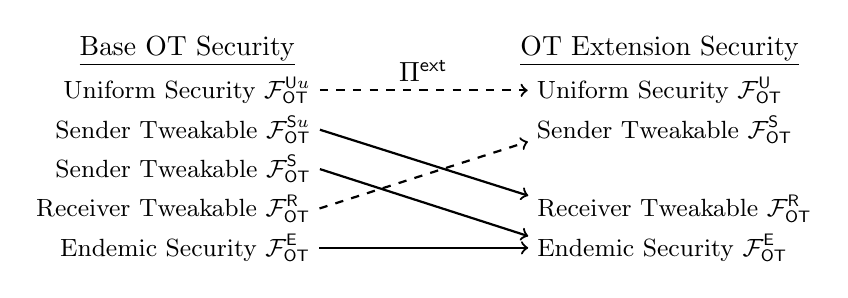
\begin{tikzpicture}[scale=0.5]\small
	\node (pi) at (6,4.5) {\normalsize $\Pi^\textsf{ext}$};
	\node (Base) at (0,5) {\underline{\normalsize Base OT Security}};
	\node (U) at (0,4) {Uniform Security $\OOT^{\U u}$};
	\node (SCu) at (-0.1,3) {Sender Tweakable $\OOT^{\send u}$};
	\node (SC) at (-0.1,2) {Sender Tweakable $\OOT^{\send}$};
	\node (RC) at (-0.35,1) {Receiver Tweakable  $\OOT^{\rec}$};
	\node (E) at (-0.05,0) {Endemic Security  $\OOT^{\E}$};
	
	
	\node (Ext) at (12,5) {\underline{\normalsize OT Extension Security}};
	\node (EU) at (12,4) {Uniform Security $\OOT^{\U}$};
	\node (ESC) at (12.13,3) {Sender Tweakable $\OOT^{\send}$};
	\node (ERC) at (12.38,1) {Receiver Tweakable  $\OOT^{\rec}$};
	\node (EE) at (12.07,0) {Endemic Security  $\OOT^{\E}$};
%	\draw [-implies,double equal sign distance] (U) -- (SC);
%	\draw [-implies,double equal sign distance] (U) -- (RC);
%	\draw [-implies,double equal sign distance] (SC) -- (E);
%	\draw [-implies,double equal sign distance] (RC) -- (E);
	\draw [->, thick, dashed] (U) -- (EU);
	\draw [->, thick] (E) -- (EE);
	\draw [->, thick] (SCu.east) -- (ERC.175);
	\draw [->, thick, dashed] (RC.east) -- (ESC.185);
	\draw [->, thick] (SC.east) -- (EE.175);
	
%	\draw [-, thick] (5,2.5)-- (TC);
%	\draw [->, thick] (E) .. controls (1,0.75) .. (SC);
%	\draw [->, thick] (E) .. controls (7,0.75) .. (RC);
	\end{tikzpicture}
	\label{fig:OTExtrelations}
	\caption{
		The figure depicts the implication different Base OT security notions (\definitionref{def:otSec}) have on the result OT extension protocol.  $A\rightarrow B$ denotes that any OT realizing security $A$ can be efficiently transformed by $\Pi^\textsf{ext}$ into an OT extension realizing security $B$, where $\Pi^\textsf{ext}$ is the protocol of \figureref{fig:otExt} such that $\OOT$ is the left hand side oracle. The dashed arrows are the same expect $\Pi^{\textsf{ext}}$ must be slightly modified. 
	}
\end{figure}

From endemic OT extension uniform message security can be achieved in several ways. One solution is the black-box transformation $\Pi^\U_{1,N}$ of \figureref{fig:uniformOT} which lifts an OT protocol with Endemic security to satisfy Uniform Message security. However, this would require additional rounds and significant communication. We demonstrate an alternative solution which replaces the base OTs with a protocol that satisfies Uniform Message, Uniform Selection security $\OOT^{\U u}$ and prove that this yields an OT extension protocol with Uniform Message security without the need to modify the extension protocol. More generally, \figureref{fig:OTExtrelations} shows the relation between different base OT security notions and the resulting OT extension message security. 
\iffullversion
For example, the protocols of \cite{C:IKNP03,EC:ALSZ15,C:KelOrsSch15} perform
$$
\OOT^\send \xrightarrow{\Pi^{\textsf{ext}}} \OOT^\E \xrightarrow{\Pi^{\send}_{1,2}} \OOT^\send
$$
where $\Pi^\textsf{ext}$ is their respective extension protocol up to hashing.
\fi

In addition, \sectionref{sec:extIdealCipher} details new OT extension protocols that can efficiently be realized in the ideal cipher model. These protocol are inspired by existing implementation \cite{libOTe,KOS,EMP} but are provably secure. Unfortunately, these existing implementation improperly apply the ideal cipher model which could be leverage by a malicious receiver to fully break \emph{all} OT messages. 
%\textcolor{red}{mention ideal cipher optimization}


\paragraph{Implementation.} We instantiate our OT protocol with the Diffie-Hellman key exchange. We show how the security loss can be reduced using the random self-reducibility of the DDH assumption. 
We also instantiate it based on the Kyber key exchange \cite{EPRINT:BDKLLS17,NISTPQC-R1:CRYSTALS-KYBER17}. This is a proof of concept instantiation that shows that our framework is very agile in terms of assumptions and allows to obtain post-quantum security efficiently. 

We give implementations and benchmarks for two OT protocols based on DDH and one based on LWE as well as five implementations of OT extension protocols. Both our OT protocols can perform an OT in one millisecond. We compare our results with the OTs of Chou \& Claudio \cite{LC:ChoOrl15} and Naor \& Pinkas \cite{SODA:NaoPin01}. In a WAN network setting we observe that our one round DDH protocol is the fastest, requiring 110ms. The next fastest framework was the two round protocol of \cite{LC:ChoOrl15}, requiring 210ms. In addition to being faster than \cite{LC:ChoOrl15} in the WAN setting, our protocols achieve full simulation based security without performing addition rounds as \cite{LC:ChoOrl15} requires. 

Our communication optimized OT extension protocol achieving endemic security requires two rounds of communication and can processes 2 million OTs per second. This is on par with a throughput optimized version of \cite{C:KelOrsSch15,libOTe} in the LAN setting. In the WAN setting our protocol becomes 2.5 times faster than \cite{C:KelOrsSch15} (which achieves stronger security). Our computation optimized protocol in the ideal cipher model can process 23 million OTs per second over the course of 5 rounds and achieves full uniform message security.



\section{Preliminaries}

\subsection{Notation}
$\sec$ denotes the security parameter and for $n\in\mathbb N$, $[n]:=\{1,\dots,n\}$. We use $\langle \A,\B\rangle$ to denote a protocol between two parties \A and \B as well as the transcript of the protocol, which consists of all the messages sent between them. We use $(\A(a),\B(b))_{\langle \A,\B\rangle}$ to denote the joint output distribution of $\A$ and \B when interacting in protocol $\langle \A,\B\rangle$ with inputs $a$ and $b$.


\begin{definition}[Random Oracle]
A \emph{random oracle} over a set of domains and an image is a collection of functions \H that map an element $q$ within one of the domains  to a uniform element $\H(q)$ in the image.  
\end{definition}


\subsection{Key Agreement}

\begin{figure}[h!]
\centering
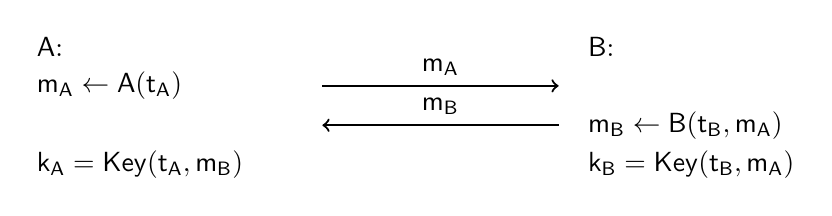
\begin{tikzpicture}
\node [anchor=west] at (0,5) {\A:};
\node [anchor=west] at (7,5) {\B:};
\node [anchor=west] at (0,4.5){$\mes_\A\leftarrow\A(\tape_\A)$};
\draw [thick, ->] (3.75,4.5)-- node [midway,above]{$\mes_\A$}(6.75,4.5);
\node [anchor=west] at (7,4){$\mes_\B\leftarrow\B(\tape_\B,\mes_\A)$};
\draw [thick, <-] (3.75,4)-- node [midway,above]{$\mes_\B$}(6.75,4);
\node [anchor=west] at (0,3.5) {$\key_\A=\EK(\tape_\A,\mes_\B)$};
\node [anchor=west] at (7,3.5) {$\key_\B=\EK(\tape_\B,\mes_\A)$};
\end{tikzpicture}
\label{fig:UKA}
\caption{The figure shows a key agreement protocol between parties \A and \B with random tapes $\tape_\A$ and $\tape_\B$. For correctness, we require $\key_\A=\key_\B$.}
\end{figure}


\begin{definition}[(Two Message) Uniform Key Agreement (\UKA)] 
Let \G be a group.
We call a protocol $\langle \A,\B\rangle$ between two ppt parties \A and \B (two message) uniform key agreement if \A first sends a message $\mes_\A\in\G$ to \B and \B responds with a final message $\mes_\B$ and in the end, both establish a common key $\key$ (see Figure~\ref{fig:UKA}) using a key establish algorithm \EK. Further, we require three properties:
\begin{description}
\item[Correctness:]
$$
\Pr[\key_\A=\EK(\tape_\A,\mes_\B)=\EK(\tape_\B,\mes_\A)=\key_\B]\geq 1-\negl,
$$
where $\tape_\A\leftarrow\bits^*$, $\tape_\B\leftarrow\bits^*$, $\mes_\A\leftarrow\A(\tape_\A)$ and $\mes_\B\leftarrow\B(\tape_\B)$.
\item [Key Indistinguishability:] For any ppt distinguisher \D,
$$ 
|\Pr[\D(1^\sec,\langle \A,\B\rangle, \key)=1]-\Pr[\D(1^\sec,\langle \A,\B\rangle, u)=1]|=\negl,
$$
where $\key$ is the established key between \A and \B and $u$ is a uniform element from the key domain.
\item [Uniformity:] For any ppt distinguisher \D, 
$$
|\Pr[\D(1^\sec,\mes_\A)=1]-\Pr[\D( 1^\sec,u)=1]|=\negl,
$$
where $u$ is a uniform element from \G.
\end{description}
When \A and \B can send their messages concurrently, we call it a $1$-round \UKA otherwise a $2$-round \UKA.
\end{definition}

\begin{definition}[Multi-Instance Uniformity]
We call a \UKA $Q$ \emph{multi-instance uniform} if for any ppt distinguisher \D,
$$
|\Pr[\D^{\O_{\A}}(1^{\sec})]=1]-Pr[\D^{\O_{u}}(1^{\sec})=1]|=\negl,
$$
where $\O_{\A}$ outputs $\mes_\A\leftarrow\A(\tape_\A)$ for fresh randomness $\tape_\A$ and $\O_u$ outputs $u\leftarrow\G$ and $Q$ is a bound on the amount of queries to $\O_{u}$, $\O_{\A}$.
\end{definition}



\begin{definition}[Multi-Instance Key Indistinguishability]
We call a \UKA $(Q,n)$ \emph{multi-instance key indistinguishable} if for any ppt distinguisher \D,
$$
|\Pr[\D^{\O_{\langle \A,\B\rangle}, \O_{\key}}(1^{\sec})]=1]-Pr[\D^{\O_{\langle \A,\B\rangle},\O_{u}}(1^{\sec})=1]|=\negl,
$$
where $\O_{\langle \A,\B\rangle}$ outputs on the $i$-th query a transcript $\T_i:=\langle \A_i,\B_i\rangle$, $\O_{\key}$ outputs on query $j$, key $\key_j=\EK(\tape_{\A_j},\mes_{\B_j})=\EK(\tape_{\B_j},\mes_{\A_j})$ that matches transcript $\T_i$. $\O_u$ outputs a uniform element $u$ from the key domain. $\O_{\langle \A,\B\rangle}$ uses fresh random tapes $\tape_{\A_i},\tape_{\B_i}\leftarrow\bits^*$ for every query. $Q$ is a bound on the amount of queries to $\O_{\langle \A,\B\rangle}$, where $n$ bounds the amount of queries to $\O_{\key}$, $\O_{u}$. 
\end{definition}

\subsection{Oblivious Transfer}



\begin{definition}[Ideal $k$ out of $n$ Oblivious Transfer]
An \emph{ideal $k$ out of $n$ oblivious transfer} is an oracle \OOT that interacts with two parties, a sender \send and a receiver \rec. It takes a subset  $\set\subseteq[n]$ of size $k$ from \rec and in the end \send outputs $n$ strings $(s_i)_{i\in[n]}$ and \rec outputs the strings $(s_i)_{i\in\set}\subset(s_i)_{i\in[n]}$. We distinguish three kinds of ideal OTs
\begin{description}
\item[Sender Chosen Ideal OT:] $\send$ chooses $(s_i)_{i\in[n]}$ and sends it to \OOT. \OOT sends $(s_i)_{i\in\set}$ to \rec. We refer to \OOT with $\OOT^{\send}$.
\item[Receiver Chosen Ideal OT:] \rec chooses $(s_i)_{i\in\set}$ and sends it to \OOT. \OOT samples the remaining strings $(s_i)_{i\in[n]}\setminus(s_i)_{i\in\set}$ uniformly at random and sends $(s_i)_{i\in[n]}$ to \send. We refer to \OOT with $\OOT^{\rec}$.
\item[Uniform Ideal OT:] \OOT samples $(s_i)_{i\in[n]}$ uniformly at random and sends $(s_i)_{i\in[n]}$ to \send and $(s_i)_{i\in\set}$ to \rec. We refer to \OOT with $\OOT^{u}$.
\end{description}
\end{definition}

\begin{definition}[$k$ out of $n$ Oblivious Transfer ($\OT_{k,n}$)]
We call a protocol $\langle \send,\rec \rangle$ between two ppt parties, a sender \send and a receiver \rec, a \emph{$k$ out of $n$ oblivious transfer} if \rec has as input a set $\set\subset[n]$ of size $k$ and at the end, \send outputs $n$ strings $(s_i)_{i\in[n]}$ and \rec outputs $(s_i)_{i\in\set}$. For security, we require two properties with respect to an ideal OT \OOT.
\begin{description}
\item[Security Against a Malicious Sender:] For any ppt adversary \Adv, there exists a ppt adversary \Adv' such that for any ppt distinguisher \D
$$
|\Pr[\D((\Adv,\rec)_{\langle \Adv, \rec\rangle})=1] -\Pr[\D( (\Adv', \O_{\OT, \rec})_{\langle \Adv', \OOT\rangle})=1]|=\negl,
$$
where $\O_{\OT, \rec}$ is the \rec's side output within the view of \OOT and all algorithms receive input $1^\sec$. \rec additionally receives input \set.
\item[Security Against a Malicious Receiver:] For any ppt adversary \Adv, there exists a ppt adversary \Adv' such that for any ppt distinguisher \D
$$
|\Pr[\D((\send, \Adv)_{\langle \send, \Adv\rangle})=1] -\Pr[\D((\O_{\OT,\send},\Adv')_{\langle \OOT , \Adv' \rangle})=1]|=\negl,
$$
where $\O_{\OT,\send}$ is  the \send's side output within the view of \OOT and all algorithms receive input $1^\sec$.
\end{description}
We distinguish four different security notions.
\begin{description}
\item[Uniform Security:] The OT is secure with respect to $\OOT^u$.
\item[Sender Tweakable Security:] The OT is secure with respect to $\OOT^{\send}$.
\item[Receiver Tweakable Security:] The OT is secure with respect to $\OOT^{\rec}$.
\item[Endemic Security:] The OT is secure against a malicious  sender with respect to $\OOT^{\send}$ and secure against a malicious receiver with respect to $\OOT^{\rec}$.
\end{description}
\end{definition}

\begin{remark}
Uniform security is the strongest security definition since a malicious party cannot tweak the distribution of the strings  $(s_i)_{i\in[n]}$. Endemic security gives the weakest security guarantees since in both cases, the malicious receiver and malicious sender case, the adversary can potentially choose the strings $(s_i)_{i\in\set}$.
\end{remark}
\section{Relations between OT Security Notions}\label{sec:relot}


\begin{lemma}\label{lemma:is_a}
Let the distribution of OT strings be efficiently sampleable. 
Then $\OOT^\U$-security implies $\OOT^{\send}$ as well as $\OOT^\rec$-security. $\OOT^{\send}$ or $\OOT^\rec$-security imply $\OOT^\E$-security.
\end{lemma}

\begin{proof}
In the first step, we show that uniform message security implies sender chosen message security and receiver chosen message security implies endemic security. These two implications result from the same simple fact that a malicious sender interacting with the ideal OT is easier to construct when it can choose the OT strings than when it receives the strings from the ideal OT. The following claim formalizes this fact. 
\begin{claim}\label{claim:utocs}
Let $\Pi$ be an OT secure against a malicious sender with respect to an ideal OT $\OOT^*$ that sends the OT strings $(s_i)_{i\in[n]}$ to the sender, i.e. functionality $\OOT^\U$ and $\OOT^{\rec}$, and the distribution of $(s_i)_{i\in[n]}$ is efficiently sampleable. Then $\Pi$ is also secure against a malicious sender with respect to ideal OT $\OOT$, which receives the OT strings $(s_i)_{i\in[n]}$ from the sender, i.e functionality $\OOT^\send$ and $\OOT^\E$.
\end{claim}


\begin{proof}
We show that if there is an adversary that breaks the security against a malicious security with respect to ideal OT $\OOT$ then there is also an adversary that breaks the security with respect to $\OOT^*$. More precisely, if there is a ppt adversary $\Adv_1$ such that for any ppt adversary $\Adv_1'$ there exists a ppt distinguisher $\D_1$ with 
$$
|\Pr[\D_1((\Adv_1,\rec)_{\Pi})=1] -\Pr[\D_1( (\Adv'_1, \OOT))=1]|=\epsilon,
$$
where all algorithms receive input $1^\sec$ and \rec additionally receives input \set.
Then there is also a ppt adversary $\Adv_2$ such that for any ppt adversary $\Adv_2'$ there exists a ppt distinguisher $\D_2$ with 
$$
|\Pr[\D_2((\Adv_2,\rec)_{\Pi})=1] -\Pr[\D_1( (\Adv'_2, \OOT^*))=1]|=\epsilon,
$$
where all algorithms receive input $1^\sec$ and \rec additionally receives input \set.

We set $\Adv_2:=\Adv_1$ and $\D_2:=\D_1$. Further, for any $\Adv_2'$, there is an $\Adv_1'$  such that the distribution of $(\Adv'_2, \OOT^*)$ is identical with the distribution $(\Adv'_1, \OOT)$. This follows from the fact that  $\Adv_1'$ could choose the OT strings $(s_i)_{i\in[n]}$  from the same distribution as $\OOT^*$ does and otherwise follow the description of $\Adv_2'$. Since $\D_1$ is successful for any $\Adv_1'$ it will be also for any $\Adv_2'$, which can be seen as a subset of the set of all ppt adversaries $\Adv_1'$.
\end{proof}

The remaining two implications, from uniform security to receiver chosen message security and from sender chosen message security to endemic security follow in a similar fashion. Again it is easier to construct a malicious receiver interacting with the ideal OT when he can choose the OT strings rather than receiving them from the ideal OT.
\begin{claim}\label{claim:utocr}
Let $\Pi$ be an OT secure against a malicious receiver with respect to an ideal OT $\OOT^*$ that sends the learned OT strings $(s_i)_{i\in\set}$ to the receiver, i.e. functionality $\OOT^\U$ and $\OOT^{\send}$, and the distribution of $(s_i)_{i\in\set}$ is efficiently sampleable. Then $\Pi$ is also secure against a malicious sender with respect to ideal OT $\OOT$, which receives the OT strings $(s_i)_{i\in\set}$ from the receiver, i.e. $\OOT^\rec$ and $\OOT^\E$.
\end{claim}

\begin{proof}
The proof is basically identical to the proof of Claim~\ref{claim:utocs}. Again, the set of all ppt $\Adv_2'$ is a subset of the set of all ppt $\Adv_1'$ and identical with the set of all $\Adv_1'$ that sample  $(s_i)_{i\in\set}$ from the same distribution as when sent by $\OOT^*$.
\end{proof}

\end{proof}











\begin{figure}[t]
\centering
\framebox{
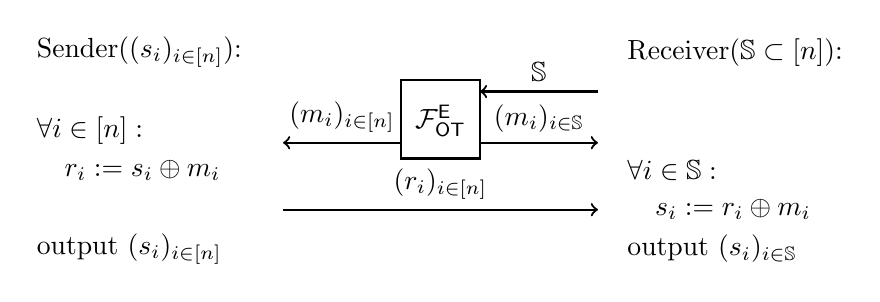
\begin{tikzpicture}
\node [anchor=west] at (0,5) {Sender$((s_i)_{i\in[n]})$:};
\node [anchor=west] at (7.5,5) {Receiver$(\set\subset[n])$:};
\draw [thick, <-] (5.75,4.5)-- node [midway,above]{$\set$}(7.25,4.5);
\draw [thick] (4.75,4.65)--(5.75,4.65)--(5.75,3.65)--(4.75,3.65)--cycle;
\node at (5.25,4.125){$\OOT^\E$};
\node [anchor=west] at (0,4){$\forall i\in[n]:$};
\node [anchor=west] at (0,3.5){$\quad r_i:=s_i\oplus m_i$};

\draw [thick, ->] (3.25,3)-- node [midway,above]{$(r_i)_{i\in[n]}$}(7.25,3);
\node [anchor=west] at (7.5,3.5){$\forall i\in\set:$};
\node [anchor=west] at (7.5,3){$\quad s_i:=r_i\oplus m_i$};
\draw [thick, ->] (5.75,3.85)-- node [midway,above]{$(m_i)_{i\in \set}$}(7.25,3.85);
\draw [thick, <-] (3.25,3.85)-- node [midway,above]{$(m_i)_{i\in [n]}$}(4.75,3.85);
\node [anchor=west] at (0,2.5) {output $(s_i)_{i\in[n]}$};
\node [anchor=west] at (7.5,2.5) {output $(s_i)_{i\in\set}$};
\end{tikzpicture}
}
% 	\framebox{\begin{minipage}{0.95\linewidth}
% 			Input: The sender $\send$ has input $s_1,...,s_n\in \{0,1\}^\ell$ while the receiver $\rec$ has input $\set\subseteq [n]$ of size $k$.
% 			\begin{enumerate}
% 				\item \label{step:senderChosen_step1} The parties invoke $\O^{e}_{k,n}$ where $\rec$ takes the role of the receiver with inputs $\set$. $\send$ obtains $(m_i)_{i\in[n]}$ and $\rec$ obtains  from  $\O^{e}_{k,n}$. 
% 				\item \label{step:senderChosen_step2}  $\send$ sends the strings $r_1,...,r_n$ to $\rec$ where $r_i:=s_i\oplus m_i$.
% 				\item \label{step:senderChosen_step3}  $\rec$ outputs $(s_i)_{i\in \set}$ where $s_i:=m_i\oplus r_i$.
% 	\end{enumerate}\end{minipage}}
	\caption{Sender Chosen OT Protocol $\Pi^{\send}_{k,n}$ in the $\OOT^\E$ hybrid (\definitionref{def:ot}). For all $i\in[n]$, $r_i$, $m_i$ and $s_i$ are in $\bits^\ell$.}
	\label{fig:protoSendOT}
\end{figure}


\begin{lemma}
	$\Pi^{\send}_{k,n}$ of \figureref{fig:protoSendOT} realizes the Sender Chosen Ideal OT $\OOT^{\send}$ (\definitionref{def:ot}) with unconditional security in the $\OOT^\E$ hybrid.
\end{lemma}

\iffullversion
\begin{proof}
 We construct a new adversary $\Adv_1'$ which interacts with functionality $\OOT^\send$ and produces an identical output  to $\Adv_1$.  $\Adv_1'$ plays the role of $\OOT^\E$ and $\rec$ in $\Pi^{\send}_{k,n}$ while running $\Adv_1$. $\Adv_1'$ receives the endemic OT strings $m_1,...,m_n$ from $\Adv_1$%in \stepref{step:senderChosen_step1}
, along with the strings $r_1,...,r_n$% in \stepref{step:senderChosen_step2}
.  $\Adv_1'$ extracts the OT strings of $\Adv_1$ as $s_i:=r_i\oplus m_i$. $\Adv_1'$ sends $(s_i)_{i\in [n]}$ to $\OOT^\send$ and outputs whatever $\Adv_1$ outputs.
	
	Observe that the output of the honest receiver is identical when $\Adv_1$ interacts with $\rec$ in $\Pi^{\send}_{k,n}$ and when $\Adv_1'$ interacts with $\OOT^\send$.
	
	
	
	Now consider a corrupt receiver $\Adv$. We construct a new adversary $\Adv_2'$ which interacts with the functionality $\OOT^\send$ and produces an identical output distribution to $\Adv_2$. $\Adv_2'$ plays the role of $\OOT^\E$ and $\send$ in $\Pi^{\send}_{k,n}$ while running $\Adv_2$. $\Adv_2'$ receives the set $\set\subset[n]$ of size $k$ and the endemic OT strings $(m_i)_{i\in \set}$ from $\Adv_2$. $\Adv_2'$ sends $\set$ to  $\OOT^\send$ and receives $(s_i)_{i\in \set}$ in response. $\Adv_2'$ computes $r_i:=s_i\oplus m_i$ for $i\in \set$ and uniformly samples $r_i\gets \{0,1\}^\ell$ for $i\in [n]\setminus \set$. $\Adv_2'$ sends $r_1,...,r_n$ to $\Adv_2$ and outputs whatever $\Adv_2$ outputs.

	The transcripts of $\Adv_2$ in these two interactions are identical except for $(r_i)_{i\in [n]\setminus \set}$. Observe that in the real interaction for $i\in [n]\setminus\set$, $r_i:=s_i\oplus m_i$, where $m_i$ is sampled uniformly at random  by functionality $\OOT^\E$ and is independent of the transcript of $\Adv_2$ (conditioned on $r_i$). Therefore sampling $r_i$ directly induces an identical distribution. 
	
	Therefore, any distinguishing advantage $\Adv_1$ or $\Adv_2$ produces in protocol $\Pi^{\send}_{k,n}$ implies that $\Adv_1'$ or $\Adv_2'$ would produce the same advantage against the instantiation of $\OOT^\E$, i.e. $\negl$.
\end{proof}
\else
\begin{proof}[sketch]	
	The case of a corrupt sender is straight forward. The simulator receives $(m_i)_{i\in[n]},(r_i)_{i\in[n]}$ from \rec and sends $(m_i\oplus r_i)_{i\in[n]}$ to $\OOT^\send$. The output distribution is identical to the real protocol. Consider a corrupt receiver. The simulator receives their set and strings $(m_i)_{i\in\in{\set}}$. All other $(m_i)_{i\in\in{[n]\setminus\set}}$ are uniformly distributed in their view. Therefore, so is $(m_i+r_i)_{i\in\in{[n]\setminus\set}}$ and the simulator can then replace these strings with $(r_i)_{i\in\in{[n]\setminus\set}}$.
\end{proof}
\fi

\begin{figure}[t]
\centering
\framebox{
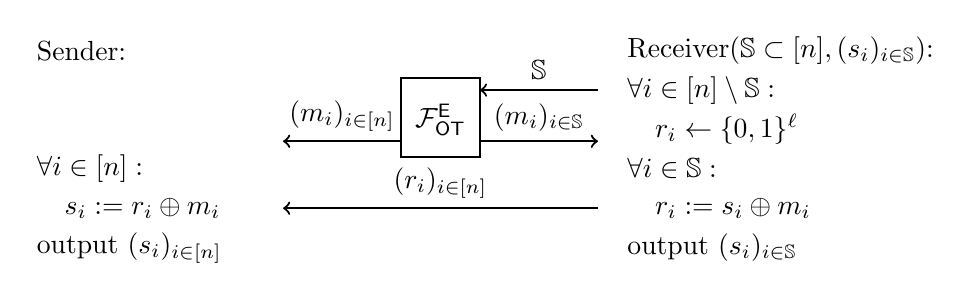
\begin{tikzpicture}
\node [anchor=west] at (0,5) {Sender:};
\draw [thick, <-] (5.75,4.5)-- node [midway,above]{$\set$}(7.25,4.5);
\node [anchor=west] at (7.5,5) {Receiver$(\set\subset[n],(s_i)_{i\in\set})$:};
\draw [thick] (4.75,4.65)--(5.75,4.65)--(5.75,3.65)--(4.75,3.65)--cycle;
\node at (5.25,4.125){$\OOT^\E$};
\node [anchor=west] at (0,3.5){$\forall i\in[n]:$};
\node [anchor=west] at (0,3){$\quad s_i:=r_i\oplus m_i$};

\draw [thick, <-] (3.25,3)-- node [midway,above]{$(r_i)_{i\in[n]}$}(7.25,3);
\node [anchor=west] at (7.5,4.5){$\forall i\in[n]\setminus\set:$};
\node [anchor=west] at (7.5,4){$\quad r_i\leftarrow\bits^\ell$};
\node [anchor=west] at (7.5,3.5){$\forall i\in\set:$};
\node [anchor=west] at (7.5,3){$\quad r_i:=s_i\oplus m_i$};
\draw [thick, ->] (5.75,3.85)-- node [midway,above]{$(m_i)_{i\in \set}$}(7.25,3.85);
\draw [thick, <-] (3.25,3.85)-- node [midway,above]{$(m_i)_{i\in [n]}$}(4.75,3.85);
\node [anchor=west] at (0,2.5) {output $(s_i)_{i\in[n]}$};
\node [anchor=west] at (7.5,2.5) {output $(s_i)_{i\in\set}$};
\end{tikzpicture}
}
% 	\framebox{\begin{minipage}{0.95\linewidth}
% 			Input: The sender $\send$ has no input while the receiver $\rec$ has input $\set\subseteq [n]$ of size $k$ and $(s_i)_{i\in \set}$ where $s_i\in \{0,1\}^\ell$.
% 			\begin{enumerate}
% 				\item \label{step:receiverChosen_step1} The parties invoke $\O^{e}_{k,n}$ where $\rec$ takes the role of the receiver with inputs $\set$. $\send$ obtains $(m_i)_{i\in[n]}$ and $\rec$ obtains $(m_i)_{i\in \set}$ from  $\O^{e}_{k,n}$. 
% 				\item \label{step:receiverChosen_step2}  $\rec$ sends the strings $r_1,...,r_n$ to $\send$ where $r_i:=s_i\oplus m_i$ for $i\in \set$ and $r_i\gets\{0,1\}^\ell$ for $i\in [n]\setminus\set$.
% 				\item \label{step:receiverChosen_step3}  $\send$ outputs $(s_i)_{i\in [n]}$ where $s_i:=m_i\oplus r_i$.
% 	\end{enumerate}\end{minipage}}
	\caption{Receiver Chosen OT Protocol $\Pi^{\rec}_{k,n}$ in the $\OOT^\E$ hybrid (\definitionref{def:ot}). For all $i\in[n]$, $r_i$, $m_i$ and $s_i$ are in $\bits^\ell$.}
	\label{fig:protoRecvOT}
\end{figure}


\begin{lemma}
	$\Pi^{\rec}_{k,n}$ of \figureref{fig:protoRecvOT} realizes the Receiver Chosen Ideal OT $\OOT^{\rec}$ (\definitionref{def:ot}) with unconditional security in the $\OOT^\E$ hybrid.
\end{lemma}
\iffullversion
\begin{proof}
	First let us consider any corrupt sender $\Adv_1$. We construct a new adversary $\Adv_1'$ which interacts with $\OOT^{\rec}$ and produces an identical output distribution as $\Adv_1$.  $\Adv_1'$ plays the role of $\OOT^\E$ and $\rec$ in $\Pi^{\rec}_{k,n}$ while running $\Adv_1$. $\Adv_1'$ receives the endemic OT strings $m_1,...,m_n$ from $\Adv_1$% in \stepref{step:receiverChosen_step1}
. $\Adv_1'$ invokes $\OOT^{\rec}$ as the sender and receives $s_1,...,s_n$ in response. $\Adv_1'$ sends $r_1,...,r_n$ to $\Adv_1$ where $r_i:=m_1\oplus s_i$ and 	 outputs whatever $\Adv_1$ outputs.
	
	The transcripts of $\Adv_1$ in these two interactions are identical except for $(r_i)_{i\in [n]\setminus \set}$. Observe that in the real interaction for $i\in [n]\setminus\set$, $r_i\gets\{0,1\}^\ell$ while $\Adv_1'$ chooses $r_i:=m_1\oplus s_i$ where $s_i$ is sampled uniformly at random by $\OOT^{\rec}$. Therefore, computing $r_i:=m_1\oplus s_i$ implies an identically distribution as when $r_i\gets\{0,1\}^\ell$ given that $s_i\gets\{0,1\}^\ell$ is independent of the transcript of $\Adv_1$. 
	
	
	Now let us consider a corrupt receiver $\Adv_2$. We construct a new adversary $\Adv_2'$ which interacts with $\OOT^{\rec}$ and produces an identical output as $\Adv_2$. $\Adv_2'$ plays the role of $\OOT^\E$ and $\send$ in $\Pi^{\rec}_{k,n}$ while running $\Adv_2$. $\Adv_2'$ receives the set $\set\subset[n]$ of size $k$ and the endemic OT strings $(m_i)_{i\in \set}$ from $\Adv_2$% in \stepref{step:receiverChosen_step1}
. $\Adv_2'$ receives $r_1,...,r_n$ from $\Adv_2$ % in \stepref{step:receiverChosen_step2} 
 and extracts $(s_i)_{i\in \set}$ as $s_i:=r_i\oplus m_i$. $\Adv_2'$ sends $\set$ and $(s_i)_{i\in \set}$ to $\OOT^{\rec}$ and outputs whatever $\Adv_2$ outputs.
	
	The output distribution of he honest sender is identical in these two interactions is identical except for $(s_i)_{i\in [n]\setminus \set}$. In the real interaction \send outputs $s_i:=m_i\oplus r_i$ where $m_i$ is sampled uniformly by $\OOT^\E$ and independent of the transcript. Therefore $\OOT^{\rec}$ sampling $s_i\gets\{0,1\}^\ell$ directly is identically distributed.
	
	Therefore, any distinguishing advantage adversary $\Adv_1$ or $\Adv_2$ produces in protocol $\Pi^{\rec}_{k,n}$ implies  that $\Adv_1'$ or $\Adv_2'$ would produce the same advantage against the instantiation of $\OOT^\E$, i.e. $\negl$.
\end{proof}
\else
\begin{proof}[sketch]
	Consider a corrupt sender. First, \send sends $(m_i)_{i\in[n]}$ to the simulator and $\OOT^\rec$ sends $(s_i)_{i\in[n]}$. $k$ of the $s_i$ strings will have a distribution specified by $\rec$ while the other are uniform. For all of them, the simulator computes $r_i:=s_i+m_i$ and sends $r_i$ to \send. For the uniform $s_i$, adding another uniform value does not change the distribution. The other messages have an identical distribution.	
	For a corrupt receiver, the $(m_i)_{i\in[n]\setminus\set}$ are uniformly distributed in their view. Therefore, so is $(m_i+r_i)_{i\in [n]\setminus\set}$. 
\end{proof}
\fi


\begin{figure}[t]
\centering
\framebox{
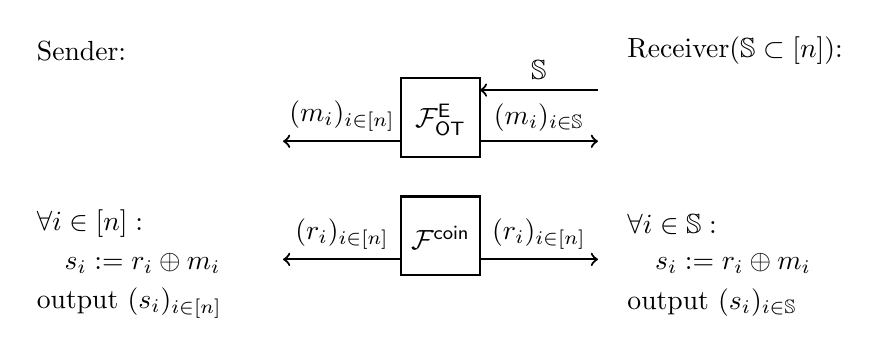
\begin{tikzpicture}
\node [anchor=west] at (0,5) {Sender:};
\node [anchor=west] at (7.5,5) {Receiver$(\set\subset[n])$:};
\draw [thick, <-] (5.75,4.5)-- node [midway,above]{$\set$}(7.25,4.5);
\draw [thick] (4.75,4.65)--(5.75,4.65)--(5.75,3.65)--(4.75,3.65)--cycle;
\node at (5.25,4.125){$\OOT^\E$};
\draw [thick, ->] (5.75,3.85)-- node [midway,above]{$(m_i)_{i\in \set}$}(7.25,3.85);
\draw [thick, <-] (3.25,3.85)-- node [midway,above]{$(m_i)_{i\in [n]}$}(4.75,3.85);
\draw [thick] (4.75,3.15)--(5.75,3.15)--(5.75,2.15)--(4.75,2.15)--cycle;
\node at (5.25,2.625){$\F^{\coin}$};
\draw [thick, ->] (5.75,2.35)-- node [midway,above]{$(r_i)_{i\in [n]}$}(7.25,2.35);
\draw [thick, <-] (3.25,2.35)-- node [midway,above]{$(r_i)_{i\in [n]}$}(4.75,2.35);

\node [anchor=west] at (0,2.8){$\forall i\in[n]:$};
\node [anchor=west] at (0,2.3){$\quad s_i:=r_i\oplus m_i$};
\node [anchor=west] at (7.5,2.8){$\forall i\in\set:$};
\node [anchor=west] at (7.5,2.3){$\quad s_i:=r_i\oplus m_i$};

\node [anchor=west] at (0,1.8) {output $(s_i)_{i\in[n]}$};
\node [anchor=west] at (7.5,1.8) {output $(s_i)_{i\in\set}$};
\end{tikzpicture}
}
% 	\framebox{\begin{minipage}{0.95\linewidth}
% 			Input: The sender \send has no input and the  receiver \rec has input $\set\subseteq [n]$ of size $k$.
% 			\begin{enumerate}
% 				\item \label{step:uniform_step1} The parties invoke $\O^{e}_{k,n}$ where $\rec$ takes the role of the receiver with inputs $\set$. \send receives $(m_i)_{i\in [n]}$ and \rec receives $(m_i)_{i\in \set}$ where $m_i\in\{0,1\}^\ell$.
% 				\item \label{step:uniform_step3} The parties invoke $\O^{\coin}$ to receive $n\ell$ coins $r_1,...,r_n\in \{0,1\}^\ell$. 
% 				\item \send outputs $(s_i)_{i\in [n]}$ and \rec outputs $(s_i)_{i\in \set}$ where $s_i:=m_i\oplus r_i$.
% 			\end{enumerate}
% 	\end{minipage}}
	\caption{ Uniform  OT Protocol $\Pi^{\U}_{k,n}$ in the $\OOT^\E,\F^{\coin}$ hybrid (\definitionref{def:ot}).  For all $i\in[n]$, $r_i$, $m_i$ and $s_i$ are in $\bits^\ell$.}
	\label{fig:uniformOT}
\end{figure}


\begin{lemma}
	$\Pi^{\U}$ of \figureref{fig:uniformOT} realizes the Uniform Ideal OT $\OOT^{\U}$ (\definitionref{def:ot}) with unconditional security in the $\OOT^\E,\F^{\coin}$ hybrid.
\end{lemma}
\iffullversion
\begin{proof}
	First let us consider any corrupt sender $\Adv_1$. We construct a new adversary $\Adv_1'$ which interacts with functionality $\OOT^{\U}$ and produces an identical output distribution as $\Adv_1$.  $\Adv_1'$ plays the role of $\OOT^\E,\F^{\coin}$ and $\rec$ in $\Pi^{\U}_{k,n}$ while running $\Adv_1$. $\Adv_1'$ receives the endemic OT strings $m_1,...,m_n$ from $\Adv_1$% in \stepref{step:uniform_step1}
.
	
	
	$\Adv_1'$ invokes $\OOT^{\U}$ as the sender and receives $s_1,...,s_n$ in response. When $\Adv_1$ invokes $\F^{\coin}$% during \stepref{step:uniform_step3}
, $\Adv_1'$ sends $r_1,...,r_n$ to $\Adv_1$ on behalf of $\F^{\coin}$ where $r_i:=m_1\oplus s_i$ and outputs whatever $\Adv_1$ outputs. Observe that $s_i$ is sampled uniformly at random by $\OOT^{\U}$ and is independent of the transcript of $\Adv_1$ (conditioned on $r_i$). Therefore computing $r_i:=m_1\oplus s_i$ induces an identical distribution as $r_i\gets\{0,1\}^\ell$.
	
	Now let us consider a corrupt receiver $\Adv_2$. We construct a new adversary $\Adv_2'$ which interacts with $\OOT^{\rec}$ and produces an identical output as $\Adv_2$. $\Adv_2'$ plays the role of $\OOT^\E,\F^{\coin}$ and $\send$ in $\Pi^{\U}_{k,n}$ while running $\Adv_2$. $\Adv_2'$ receives the set $\set\subset[n]$ of size $k$ and the endemic OT strings $(m_i)_{i\in \set}$ from $\Adv_2$% in \stepref{step:uniform_step1}
. 
	
	
	$\Adv_2'$ invokes  $\OOT^{\U}$ as the receiver with input $\set$ and receives $(s_i)_{i\in\set}$ in response. When $\Adv_2$ invokes $\F^{\coin}$% during \stepref{step:uniform_step3} 
	$\Adv_2'$ sends $r_1,...,r_n$ to $\Adv_1$ on behalf of $\F^{\coin}$ where $r_i:=m_1\oplus s_i$ for $i\in \set$ and otherwise sets $r_i$ as the output of $\F^\coin$. $\Adv_2'$ outputs whatever $\Adv_2$ outputs.
	
	The transcripts of these two interactions are identical except for the messages $(r_i)_{i\in \set}$. In the real interaction $r_i$ is sampled uniformly at random by $\F^{\coin}$ as opposed to $\Adv_2'$ computing $r_i:=m_i\oplus s_i$. Observe that $s_i$ is sampled uniformly at random by $\OOT^{\U}$ and is independent of the transcript of $\Adv_2$ (conditioned on $r_i$). Therefore computing $r_i:=m_1\oplus s_i$ induces an identical distribution as $r_i\gets\{0,1\}^\ell$.

	Therefore, any distinguishing advantage adversary $\Adv_1$ or $\Adv_2$ produces in protocol $\Pi^{\U}$ implies that $\Adv_1'$ or $\Adv_2'$ would produce the same advantage against the instantiation of $\OOT^\E$ or $\F^\coin$, i.e. $\negl$.
	
\end{proof}
\else
\begin{proof}[sketch]
	Consider a corrupt \send. The simulator calls $\OOT^{\U}$ and receives $s_1,...,s_n$. When \send invokes $\F^{\coin}$, $\Adv_1'$ sends $r_i:=m_1\oplus s_i$ to $\Adv_1$ on behalf of $\F^{\coin}$. Due to $s_i$ is sampled uniformly this change results in the same distribution. 
	For a corrupt receiver, the simulator effectively does the same. First receive $\set$ and send it to $\OOT^{\U}$ and receive $(s_i)_{i\in\set}$. Then have  $\F^{\coin}$ output $r_i:=m_1\oplus s_i$ for $i\in\set$ and uniform otherwise.
\end{proof}
\fi























\begin{figure}[t]
\centering
\framebox{
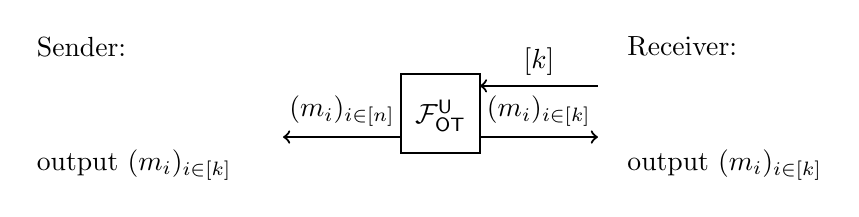
\begin{tikzpicture}
\node [anchor=west] at (0,5) {Sender:};
\node [anchor=west] at (7.5,5) {Receiver:};
\draw [thick] (4.75,4.65)--(5.75,4.65)--(5.75,3.65)--(4.75,3.65)--cycle;
\node at (5.25,4.125){$\OOT^\U$};
\draw [thick, <-] (5.75,4.5)-- node [midway,above]{$[k]$}(7.25,4.5);
\draw [thick, ->] (5.75,3.85)-- node [midway,above]{$(m_i)_{i\in [k]}$}(7.25,3.85);
\draw [thick, <-] (3.25,3.85)-- node [midway,above]{$(m_i)_{i\in [n]}$}(4.75,3.85);
\node [anchor=west] at (0,3.5) {output $(m_i)_{i\in[k]}$};
\node [anchor=west] at (7.5,3.5) {output $(m_i)_{i\in[k]}$};
\end{tikzpicture}
}
% 	\framebox{\begin{minipage}{0.95\linewidth}
% 			Input: The sender \send and receiver \rec have no input.
% 			\begin{enumerate}
% 				\item \label{step:coin_step1} \rec sends $\set:=[k]$ to $\O^{u}_{k,n}$ and receives $(s_i)_{i\in \set}$ in response. \send receives $(s_i)_{i\in [n]}$. 
% 				\item \label{step:coin_step2} Both parties output the bits of $(s_i)_{i\in [k]}$.
% 			\end{enumerate}
% 	\end{minipage}}
	\caption{Coin flipping Protocol $\Pi^{\coin}$ in the $\OOT^{\U}$ hybrid. For all $i\in[n]$, $m_i$ is in $\bits^\ell$.}
	\label{fig:coinFlip}
\end{figure}


\begin{lemma}
	$\Pi^{\textsf{coin}}$ of \figureref{fig:coinFlip} realizes an ideal coin flipping protocol with unconditional security  in the $\O^{\U}$ hybrid  (\definitionref{def:ot}).
\end{lemma}
\begin{proof}
	Trivial.
\end{proof}


\begin{figure}[t]
\centering
\framebox{
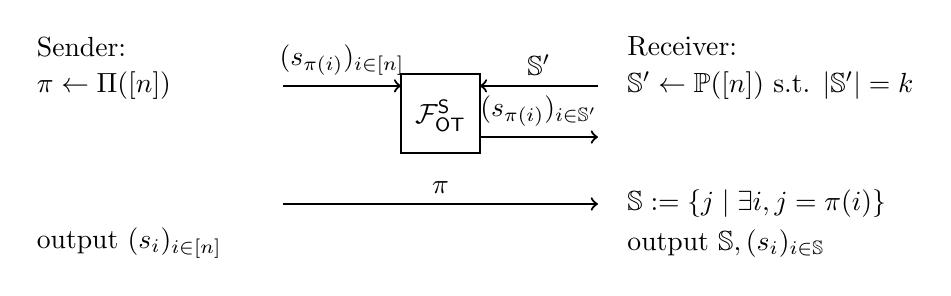
\begin{tikzpicture}
\node [anchor=west] at (0,5) {Sender:};
\node [anchor=west] at (7.5,5) {Receiver:};
\draw [thick] (4.75,4.65)--(5.75,4.65)--(5.75,3.65)--(4.75,3.65)--cycle;
\node at (5.25,4.125){$\OOT^\send$};
\node [anchor=west] at (7.5,4.5){$\set'\gets \mathbb{P}([n])$ s.t. $|\set'|=k$};
\draw [thick, <-] (5.75,4.5)-- node [midway,above]{$\set'$}(7.25,4.5);
\draw [thick, ->] (5.75,3.85)-- node [midway,above]{$(s_{\pi(i)})_{i\in \set'}$}(7.25,3.85);
\node [anchor=west] at (0,4.5) {$\pi\leftarrow\Pi([n])$};
\draw [thick, ->] (3.25,3)-- node [midway, above]{$\pi$} (7.25,3);
\draw [thick, ->] (3.25,4.5)-- node [midway,above]{$(s_{\pi(i)})_{i\in [n]}$}(4.75,4.5);
\node [anchor=west] at (0,2.5) {output $(s_{i})_{i\in[n]}$};
\node [anchor=west] at (7.5,3) {$\set:=\{j \mid \exists i, j=\pi(i)\}$};
\node [anchor=west] at (7.5,2.5) {output $\set, (s_i)_{i\in\set}$};
\end{tikzpicture}
}
% 	\framebox{\begin{minipage}{0.95\linewidth}
% 			Input: The sender \send and receiver \rec have no input.
% 			\begin{enumerate}
% 				\item \label{step:uniformSelect_step1} \rec uniformly samples $\set'\gets \mathbb{P}([n])$ s.t. $|\set'|=k$. \rec sends $\set'$ to $\OOT^{\E}$ and receives $(s_i')_{i\in \set'}$ in response. \send receives $(s_i')_{i\in [n]}$. 
% 				\item \label{step:uniformSelect_step2} \send samples a random permutation $\pi : [n] \rightarrow [n]$ and sends it to \rec.
% 				\item \label{step:uniformSelect_step3} \send outputs $(s_i)_{i\in [n]}$ and \rec outputs $(\set, (s_i)_{i\in\set})$ where $s_i:=s_{\pi(i)}'$ and $\set:=\{j \mid \exists i, j=\pi(i)\}$.
% 			\end{enumerate}
% 	\end{minipage}}
	\caption{Uniform Selection $k$-out-of-$n$ OT protocol $\Pi^{\send u}$ in the $\OOT^{\send}$ hybrid. $\Pi([n])$ is the set of permutations over $[n]$.}
	\label{fig:uniformSelect}
\end{figure}


\begin{lemma}
	$\Pi^{\E u}$ of \figureref{fig:uniformSelect} realizes the  Ideal Uniform Selection Endemic Message OT $\OOT^{\send u}$ (\definitionref{def:ot}) with unconditional security in the $\OOT^{\send}$ hybrid.
\end{lemma}


\begin{proof}[sketch]
	Consider a corrupt \send. Due to $\set'$ being uniformly distributed, so is $\set=\pi(\set')$ since $\pi$ is one to one. Consider a corrupt \rec. The simulator receives $\set'$ from \rec and the $\set,(s_i)_{i\in\set}$ from $\OOT^{\send u}$. The simulator uniformly samples $\pi$ s.t. $\{s_i\}_{i\in\set} =\{s_{\pi(i)}\}_{i\in\set'}$ and completes the protocol.
\end{proof}

\begin{remark}
	The same transformation applies to $\OOT^\U,\OOT^\E, \OOT^\rec$ except \send does not input anything to $\OOT^*$.
\end{remark}
 


% \begin{figure}[t]
% \centering
% \framebox{
% \begin{tikzpicture}
% \node [anchor=west] at (0,5.5) {Sender:};
% \node [anchor=west] at (7.5,5.5) {Receiver:};
% \draw [thick] (4.75,4.65)--(5.75,4.65)--(5.75,3.65)--(4.75,3.65)--cycle;
% \node at (5.25,4.125){$\OOT^{\rec}$};
% \draw [thick, <-] (5.75,4.5)-- node [midway,above]{$\set,(s_i)_{i\in\set}$}(7.25,4.5);
% \draw [thick, ->] (5.75,3.85)-- node [midway,above]{$(m_i)_{i\in \set'}$}(7.25,3.85);
% \node [anchor=west] at (0,3.5) {$\forall i\in[n]$};
% \node [anchor=west] at (0,3) {$\quad s_i:=H(s,m_i)$};
% \draw [thick, ->] (3.25,5)-- node [midway, above]{$c:=\com(s)$} (7.25,5);
% \draw [thick, ->] (3.25,3)-- node [midway, above]{$\open(c)$} (7.25,3);
% \node [anchor=west] at (0,5) {$s\leftarrow\bits^\sec$};
% \draw [thick, <-] (3.25,3.85)-- node [midway,above]{$(m_i)_{i\in [n]}$}(4.75,3.85);
% \node [anchor=west] at (0,2) {output $(s_i)_{i\in[n]}$};
% \node [anchor=west] at (7.5,2) {output $(s_i)_{i\in\set}$};
% \node [anchor=west] at (7.5,3) {$\forall i\in\set$};
% \node [anchor=west] at (7.5,2.5) {$\quad s_i:=H(s,m_i)$};
% \end{tikzpicture}
% }
% % 	\framebox{\begin{minipage}{0.95\linewidth}
% % 			Input: The sender \send and receiver \rec have no input.
% % 			\begin{enumerate}
% % 				\item \label{step:uniformSelect_step1} \rec uniformly samples $\set'\gets \mathbb{P}([n])$ s.t. $|\set'|=k$. \rec sends $\set'$ to $\OOT^{\E}$ and receives $(s_i')_{i\in \set'}$ in response. \send receives $(s_i')_{i\in [n]}$. 
% % 				\item \label{step:uniformSelect_step2} \send samples a random permutation $\pi : [n] \rightarrow [n]$ and sends it to \rec.
% % 				\item \label{step:uniformSelect_step3} \send outputs $(s_i)_{i\in [n]}$ and \rec outputs $(\set, (s_i)_{i\in\set})$ where $s_i:=s_{\pi(i)}'$ and $\set:=\{j \mid \exists i, j=\pi(i)\}$.
% % 			\end{enumerate}
% % 	\end{minipage}}
% 	\caption{Uniform $k$-out-of-$n$ OT protocol $\Pi^{\U}_{k,n}$ in the $\OOT^{\rec}$ hybrid and random oracle model.}
% 
% \label{fig:RtoU}
% \end{figure}


\begin{lemma}\label{lem:nosendtweak}
There is no sender tweakable secure two message OT where the sender sends its message first. 
\end{lemma}



\begin{proof}
We show that the most general notion of OT, one out of two OT is impossible.  
For a two message OT where the sender sends its message first, the sender's message $\mes_{\send}$ is a function $f_{\send}$ on input $\tape_{\send}$ and some auxiliary input $\aux$. A sender could sample $s_0,s_1$ during the protocol or receive them as input. We use $\aux$ to cover the second case. Further, there is a function $f_{\rec}$ that takes the random tape $\tape_{\rec}$, $\mes_{\send}$ and choice bit $b$ of $\rec$. Finally, there are two functions $f_{\OT,\send}(\tape_{\send},\mes_{\rec},\aux)$ that outputs $(s_0,s_1)$ and $f_{\OT,\rec}(\tape_{\rec},\mes_{\send},b)$ that outputs $s_b$. 

First, we assume that \send is committed to $(s_0,s_1)$ given $\mes_{\send}$, i.e. there is a $(s_0,s_1)$ such that
$$
\Pr_{\mes_{\rec}, (\tape_{\send},\aux)}[f_{\OT,\send}(\tape_{\send},\mes_{\rec},\aux)=(s_0,s_1)\mid \mes_{\send}=f_{\send}(\tape_{\send},\aux)]\geq\frac{3}{4}.
$$

In this case, a malicious receiver can break the security as follows. It selects two random tapes $\tape_{\rec,1}$, $\tape_{\rec,2}$, two choice bits $b_1=0$, $b_2=1$ and computes for all $i\in[2]$, $\mes_{\rec,i}= f_{\rec}(\tape_{\rec,i},\mes_{\send},b_i)$ and $s_{b_{i},i}=f_{\OT,\rec}(\tape_{\rec,i},\mes_{\send},b_i)$. It outputs $(s_{0,1},s_{1,2})$ as a guess for $s_0,s_1$.

Let the scheme be $\delta$ correct, for $\delta\geq 1-\negl$. Then, the probability that the first malicious receiver reconstructs $(s_0,s_1)$ correctly is lower bounded using Jensen's inequality by
$$
\Pr[(s_{0,1},s_{1,2})=(s_0,s_1)]\geq \left(\frac{3}{4}\delta\right)^2> \frac{1}{2},
$$
where $(s_0,s_1)=f_{\OT,\send}(\tape_{\send},\mes_{\rec},\aux)$. A malicious receiver interacting with the ideal \OT can achieve this at most with probability $\frac{1}{2}$. Hence, there is a distinguisher that breaks the sender tweakable security of the OT.

Now assume that for any $(s_0,s_1)$,
\begin{eqnarray}\label{eqn:noncomm}
\Pr_{\mes_{\rec}, \tape_{\send}}[f_{\OT,\send}(\tape_{\send},\mes_{\rec},\aux)=(s_0,s_1)\mid \mes_{\send}=f_{\send}(\tape_{\send},\aux)]<\frac{3}{4}.
\end{eqnarray}
In this case, we show that a malicious receiver can tweak the distribution of $s_0,s_1$.
The malicious receiver uses a hardwired pseudorandom function (PRF) key $\key$ for a PRF $\PRF$ that outputs a single bit.\footnote{OT implies one-way functions and hence also PRFs.} The malicious receiver samples two random tapes $\tape_{\rec,1}$, $\tape_{\rec,2}$, two uniform choice bits $b_1$, $b_2$, computes for all $i\in[2]$ $\mes_{\rec,i}=f_{\rec}(\tape_{\rec,i},\mes_{\send},b_i)$ and $s_{b_i,i}=f_{\OT,\rec}(\tape_{\rec,i},\mes_{\send},b_i)$. If $\PRF_{\key}(s_{b_1,1})=0$ it sends $\mes_{\rec,1}$ to \send and outputs $s_{b_1,1}$ otherwise it sends $\mes_{\rec, 2}$ to \send and outputs $s_{b_2,2}$

 We first give a bound on the probability that $\PRF_{\key}(s_{b_i,i})=0$. Let $\epsilon_{\PRF}$ be a probability such that
$$
\Pr[\PRF_{\key}(s_{b_i,i})=0]= \frac{1}{2}-\epsilon_{\PRF}.
$$
Then there is a distinguisher $\D$ that simply outputs $1$ if $\PRF_{\key}(s_{b_i,i})=0$. Hence,
$$
|\Pr[\D(1^\sec,s_{b_i,i},\PRF_{\key}(s_{b_i,i}))=1]-\Pr[\D(1^\sec,s_{b_i,i},u)=1]|=\epsilon_{\PRF},
$$  
where $u\leftarrow\bits$. Since $\D$ breaks \PRF with probability $\epsilon_{\PRF}$ and \PRF is secure, $\epsilon_{\PRF}$ is negligible. By $(\ref{eqn:noncomm})$, it holds with at least probability $\frac{3}{16}$ that $s_{b_1,1}\neq s_{b_2,2}$. Therefore, the probability that for the output $s_{b_i,i}$ of the malicious holds $\PRF_{\key}(s_{b_i,i})=0$ is at least
\begin{eqnarray*}
\lefteqn{\Pr[\PRF_{\key}(s_{b_i,i})=0]}\\
&=&\Pr[\PRF_{\key}(s_{b_1,1})=0]+\Pr[\PRF_{\key}(s_{b_1,1})=1\wedge\PRF_{\key}(s_{b_2,2})=0]\\
&\geq&  \left(\frac{1}{2}-\epsilon_{\PRF}\right)+\left(\frac{1}{2}+\epsilon_{\PRF}\right)\cdot\frac{3}{16}\left(\frac{1}{2}-\epsilon_{\PRF}\right)\\
&=& \frac{1}{2}+\frac{1}{64}-\negl.
\end{eqnarray*}
Since the OT is $\delta=1-\negl$ correct, we get by using a union bound that the malicious receivers output $s_{b_i,i}$ is correct and $\PRF_{\key}(s_{b_i,i})=0$ holds at least with probability $\frac{1}{2}+\frac{1}{64}-\negl$. Hence, $\PRF_{\key}(s_{b_i,i})=0$ holds with a noticeable bias - given $\key$- when the malicious receiver interacts with an honest sender. If there is a distribution of $(s_0,s_1)$ from which the ideal OT samples with the same bias, then there is a distinguisher $\D$ that breaks the security of \PRF. $\D$ samples from this distribution, queries $\PRF$ on the samples and outputs $1$ if the query returns $0$. 

Since there is no such a distribution for a secure PRF, there is no adversary $\Adv'$ that creates the same output distribution when interacting with the ideal OT as when the malicious receiver interacts with the honest sender. Hence, the OT is not sender tweakable secure. 
\end{proof}

\begin{lemma}
There is no receiver tweakable secure two message OT where the receiver sends its message first.
\end{lemma}

\begin{proof}
Again, we rule out the most general notion of OT, one out of two OT. We follow a similar strategy as in the previous lemma.
A two message OT where the receiver sends its message first has the following structure. The receiver's message $\mes_{\rec}$ is a function $f_{\rec}$ on input $\tape_{\rec}$, $b$ and some auxiliary input $\aux$. Further, there is a function $f_{\send}$ that takes the random tape $\tape_{\send}$ and $\mes_{\rec}$ as input. Finally, there are two functions $f_{\OT,\send}(\tape_{\send},\mes_{\rec})$ that outputs $(s_0,s_1)$ and $f_{\OT,\rec}(\tape_{\rec},\mes_{\send},b,\aux)$ that outputs $s_b$. 

We distinguish two cases. In case one,  we assume that \rec is committed to $s_b$ given $\mes_{\rec}$, i.e. there is a $s_b$ such that
$$
\Pr_{\mes_{\send}, (\tape_{\rec},b,\aux)}[f_{\OT,\rec}(\tape_{\rec},\mes_{\send},b,\aux)=s_b\mid \mes_{\rec}=f_{\rec}(\tape_{\rec},b,\aux)]=\frac{3}{4}+\alpha,
$$
for $\alpha\geq 0$.
Further, $s_{\overline b}$ should not be determined by $\mes_{\rec}$. Let $\ell$ be the length of $s_0$, $s_1$, then if there is a $s_{\overline b}$ s.t. 
$$
\Pr_{\tape_{\send}}[s_{\overline b}\text{ is output of }f_{\OT,\send}(\tape_{\send},\mes_{\rec})\text{ for bit }\overline b\mid \mes_{\rec}]=\frac{1}{2^\ell}+\epsilon,
$$
then a malicious receiver can sample $\tape_{\send}$ and compute $f_{\OT,\send}(\tape_{\send},\mes_{\rec})$ to learn $s_{\overline b}$ with probability $\frac{1}{2^\ell}+\epsilon-(1-\delta)$, where OT is $\delta=1-\negl$ correct. Since the ideal primitive samples $s_{\overline b}$ at uniform, the malicious receiver breaks the OT with probability $\epsilon-\negl$. Therefore, $\epsilon=\negl$. 

But now, a malicious sender can sample two random tapes $\tape_{\send,1}$, $\tape_{\send,2}$
and compute for all $i\in[2]$, $(s_{0,i},s_{1,i})=f_{\OT,\send}(\tape_{\send,i},\mes_{\rec})$ and checks for all $i\in\bits$ whether $s_{i,1}=s_{i,2}$. It outputs a random $b'$ if it holds for both or no $i\in\bits$, otherwise it outputs $b'$ such that $s_{b',1}=s_{b',2}$. It holds that
$$
\Pr[s_{b,1}=s_{b,2}]= \left(\frac{3}{4}+\alpha\right)^2+\left(\frac{1}{4}-\alpha\right)^2\frac{1}{2^\ell-1}\\
\geq \frac{9}{16}
$$
%\frac{9}{16}+\frac{1}{16(n-1)}+\frac{3(n-1)+1}{2(n-1)}\alpha+\frac{n}{n-1}\alpha^2
and
$$
\Pr[s_{\overline{b},1}=s_{\overline{b},2}]\geq \frac{1}{2^\ell}-\epsilon.
$$
Therefore,
\begin{eqnarray*}
\lefteqn{\Pr[b=b']}\\
&=&\frac{1}{2}\Pr[\nexists! i:s_{i,1}= s_{i,2}]+\Pr[s_{b,1}=s_{b,2}\wedge s_{\overline b,1}\neq s_{\overline b,2}]-(1-\delta)\\
&\geq& \frac{2^\ell-1}{2^{\ell+1}}-\frac{2^\ell-2}{2^{\ell+1}}\Pr[s_{b,1}=s_{b,2}]+\frac{2^\ell-1}{2^\ell}\Pr[s_{b,1}=s_{b,2}]
-\negl\\
&\geq & \frac{2^{\ell}-1}{2^{\ell+1}}+\frac{2^{\ell}}{2^{\ell+1}}\frac{9}{16}-\negl\geq
\frac{1}{2}+\frac{1}{32}-\frac{1}{2^{\ell+1}}+\frac{1}{4}-\negl
\end{eqnarray*}
where we apply a union bound to argue that the outputs are correct and corresponds to the receivers choice. Given that $\ell\geq 1$, the malicious sender guesses $b$ correctly with at least probability $\frac{1}{2}+\frac{1}{32}-\negl$. Since in the ideal model, an adversary can guess $b$ only with probability $\frac{1}{2}$, this constitutes a break of receiver tweakable security.

In the case two, for any $s_b$,
$$
\Pr_{\mes_{\send}, (\tape_{\rec},b,\aux)}[f_{\OT,\rec}(\tape_{\rec},\mes_{\send},b,\aux)=s_b\mid \mes_{\rec}=f_{\rec}(\tape_{\rec},b,\aux)]<\frac{3}{4}.
$$
Similar as in the proof of Lemma~\ref{lem:nosendtweak}, we argue that a malicious sender can tweak the output distribution of $(s_0,s_1)$. Due to the similarity, we only exhibit a brief version. Again we hardwire a PRF key $\key$ for a PRF with a single output bit. Given $\mes_{\rec}$, the malicious sender samples two random tapes $\tape_{\send, 1}$ and $\tape_{\send,2}$, computes for all $i\in[2]$ $(s_{0,i},s_{0,i})=f_{\OT,\send}(\tape_{\send,i},\mes_{\rec})$. If $\PRF_{\key}(s_{0,1},s_{1,1})=0$ output $(s_{0,1},s_{1,1})$ and send $\mes_{\send,1}=f_{\send}(\tape_{\send,1},\mes_{\rec})$ to \rec. Otherwise output $(s_{0,2},s_{1,2})$ and send $\mes_{\send,2}=f_{\send}(\tape_{\send,2},\mes_{\rec})$ to \rec. This way, $\Pr_{\key}(s_0,s_1)=0$ holds for the malicious sender's output $(s_0,s_1)$ with probability 
\begin{eqnarray*}
\lefteqn{\Pr[\PRF_{\key}(s_0,s_1)=0]}\\
&=&\Pr[\PRF_{\key}(s_{0,1},s_{1,1})=0]+\Pr[\PRF_{\key}(s_{0,1},s_{1,1})=1\wedge\PRF_{\key}(s_{0,2},s_{1,2})=0]\\
&\geq&  \left(\frac{1}{2}-\epsilon_{\PRF}\right)+\left(\frac{1}{2}+\epsilon_{\PRF}\right)\cdot\frac{3}{8}\left(\frac{1}{2}-\epsilon_{\PRF}\right)\\
&=& \frac{1}{2}+\frac{1}{32}-\negl,
\end{eqnarray*}
unless one breaks the security of the prf. As previously, this constitutes an attack against the receiver tweakable security.
\end{proof}
\section{From Key Agreement to Oblivious Transfer}\label{sec:endemicOT}




\begin{figure}[h!]
\centering
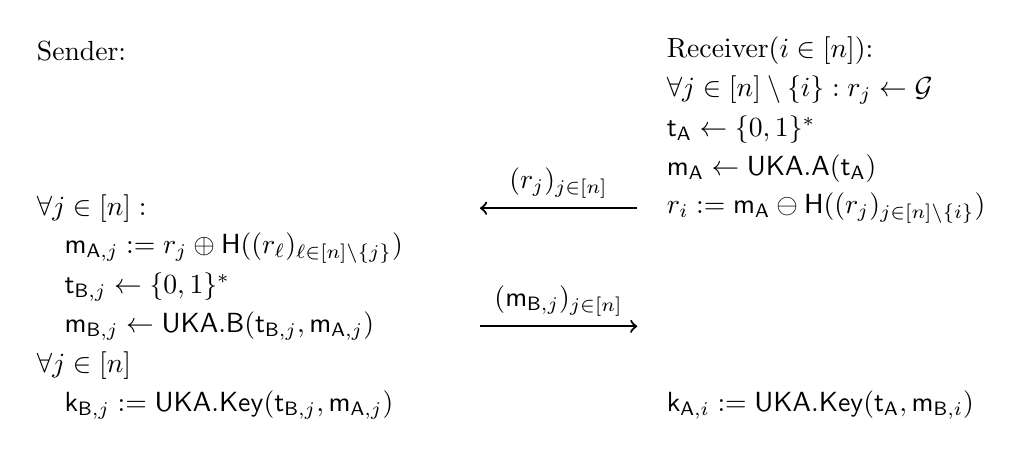
\begin{tikzpicture}
\node [anchor=west] at (-1,5) {Sender:};
\node [anchor=west] at (7,5) {Receiver$(\i\in[n])$:};
\node [anchor=west] at (7,4.5){$\forall j\in[n]\setminus\{\i\}: r_{j}\leftarrow\G$};
\node [anchor=west] at (7,4){$\tape_\A\leftarrow\bits^*$};
\node [anchor=west] at (7,3.5){$\mes_\A\leftarrow \UKA.\A(\tape_\A)$};
\node [anchor=west] at (7,3){$r_{\i}:=\mes_\A\ominus\H((r_j)_{j\in[n]\setminus\{\i\}})$};
\draw [thick, <-] (4.75,3)-- node [midway,above]{$(r_j)_{j\in[n]}$}(6.75,3);
\node [anchor=west] at (-1,3){$\forall j\in[n]:$};
\node [anchor=west] at (-1,2.5){$\quad\mes_{\A,j}:=r_j\oplus\H((r_\ell)_{\ell\in[n]\setminus\{j\}})$};
\node [anchor=west] at (-1,2){$\quad\tape_{\B,j}\leftarrow\bits^*$};
\node [anchor=west] at (-1,1.5){$\quad\mes_{\B,j}\leftarrow\UKA.\B(\tape_{\B,j},\mes_{\A,j})$};
\draw [thick, ->] (4.75,1.5)-- node [midway,above]{$(\mes_{\B,j})_{j\in[n]}$}(6.75,1.5);
\node [anchor=west] at (7,0.5) {$\key_{\A,\i}:=\UKA.\EK(\tape_\A,\mes_{\B,\i})$};
\node [anchor=west] at (-1,1) {$\forall j\in[n]$};
\node [anchor=west] at (-1,0.5) {$\quad\key_{\B,j}:=\UKA.\EK(\tape_{\B,j},\mes_{\A,j})$};
\end{tikzpicture}
\label{fig:KAtoOT}
\caption{The figure depicts a $1$ out of $n$ oblivious transfer using as a building block a \UKA and a random oracle $\H:\G^{n-1}\rightarrow\G$, where \G is a group with group operations $\oplus$, $\ominus$. By the correctness of the \UKA scheme, $\key_{\A,\i}=\key_{\B,\i}$ holds.}
\end{figure}


\begin{theorem}
Given a correct and secure \UKA scheme, then the $1$ out of $n$ oblivious transfer in Figure~\ref{fig:KAtoOT} is an Endemic $\OT_{1,n}$ in the programmable random oracle model.
\end{theorem}

\begin{proof}
We start with proving that the scheme is secure against a malicious sender. 
\begin{claim}\label{claim:malsender}
Given a $\delta$ correct and $\epsilon$ $(n-1)$-multi instance uniform \UKA scheme, then it holds that in the programmable random oracle model for any ppt adversary \Adv, there exists a ppt adversary \Adv' such that for any ppt distinguisher \D
$$
|\Pr[\D((\Adv,\rec)_{\langle \Adv, \rec\rangle})=1] -\Pr[\D( (\Adv', \O_{\OT, \rec}^\send)_{\langle \Adv', \OOT^\send\rangle})=1]|\leq \epsilon+(1-\delta),
$$
where $\O_{\OT, \rec}^\send$ is the \rec's side output within the view of $\OOT^\send$ and all algorithms receive input $1^\sec$. \rec additionally receives input \set.
\end{claim}

\begin{proof}
We define $\Adv'$ as follows. 
It generates $(r_j)_{j\in[n]}$ by sampling $r_1,\dots, r_n\leftarrow \G$. Then, it samples for all $j\in[n]$, $\tape_{\A,j}\leftarrow\bits^*$ and $\mes_{\A,j}\leftarrow\UKA.\A(\tape_{\A,j})$. Finally it programs the random oracle for all of the $j\in[n]$ points $(r_i)_{i\in[n]\setminus \{j\}}$ such that $r_i\oplus\H((r_i)_{i\in[n]\setminus \{j\}})=\mes_{\A,i}$. Now $\Adv'$ invokes \Adv, answers his random oracle queries straightforwardly, sends $(r_j)_{j\in[n]}$ and receives $(\mes_{\B,j})_{j\in[n]}$ from \Adv. It computes $s_{\A,j}\leftarrow\UKA.\EK(\tape_{\A,j},\mes_{\B,j})$ for all $j\in[n]$ and submits $(s_{\A,j})_{j\in [n]}$ to \OOT. $\Adv'$ outputs the output of \Adv.

We show, that if there is a distinguisher \D that distinguishes the distribution $(\Adv,\rec)_{\langle \Adv, \rec\rangle}$ from $(\Adv',\O_{\OT, \rec})_{\langle \Adv', \OOT\rangle}$, then there is an distinguisher $\D_{\UKA}$ against the $n$-multi instance uniformity of the \UKA scheme. 

$\D_{\UKA}$ has access to an oracle $\O$ that either outputs uniform strings or messages of the \UKA protocol. For all $j\in[n]\setminus\{i\}$, $\D_{\UKA}$ follows the description of $\Adv'$ with the difference that instead of sampling  $\mes_{\A,j}\leftarrow\UKA.\A(\tape_{\A,j})$, it samples $\mes_{\A,j}$ from $\O$. Given $(r_j)_{j\in[n]\setminus\{i\}}$, it samples $\mes_{\A,i}\leftarrow\UKA.\A(\tape_{\A,i})$ and sets $r_i$ such that $r_i\oplus\H((r_j)_{j\in[n]\setminus \{i\}})=\mes_{\A,i}$. As $\Adv'$, it computes $s_{\A,i}\leftarrow\UKA.\EK(\tape_{\A,i},\mes_{\B,i})$ which is \rec's output. It now invokes distinguisher \D on \rec's output $s_{\A,i}$ and the output of $\Adv$. In the end, it outputs the output of \D.


We now analyze the distributions. 
First, notice that the distribution of $(r_i,\mes_{A,i})$ when sampling $r_i\leftarrow\G$ and then programming the random oracle $r_i\oplus\H((r_i)_{i\in[n]\setminus \{j\}})=\mes_{\A,i}$ is identical to the distribution when sampling $\H((r_i)_{i\in[n]\setminus \{j\}})$ and choosing $r_i$  such that $r_i\oplus\H((r_i)_{i\in[n]\setminus \{j\}})=\mes_{\A,i}$, both are the uniform distribution over $\G\times\G$ conditioned to their sum being $\mes_{\A,i}$. Therefore it follows straightforwardly from the definition of \O, \rec and $\Adv'$ that when \O outputs uniform messages, the output of \Adv is distributed as when interacting with $\rec$ while when \O outputs \UKA messages, it is distributed as the output of $\Adv'$. Hence, if there is a distinguisher $\D$ that distinguishes the output distribution of \Adv given $s_{\A,i}$, i.e.
$$
\epsilon_{\D}\leq |\Pr[\D((\Adv,s_{\A,i})_{\D_{{\UKA}^{\O_\A}}})=1]-\Pr[\D((\Adv,s_{\A,i})_{\D_{{\UKA}^{\O_u}}})=1]|
$$
then it implicitly breaks the $(n-1)$-multi instance uniformity of the \UKA protocol, i.e. 
\begin{eqnarray*}
\epsilon&:=& |\Pr[\D_{\UKA}^{\O_{\A}}(1^\sec))=1] -\Pr[ \D_{\UKA}^{\O_u}(1^\sec)=1]|\\
&=&|\Pr[\D((\Adv,s_{\A,i})_{\D_{\UKA}^{\O_{\A}}})=1] -\Pr[ \D((\Adv,s_{\A,i})_{\D_{\UKA}^{\O_{u}}})=1]|\\
&\geq & \epsilon_{\D}.
\end{eqnarray*}

For finishing the proof of the claim, we now need to show that given the output of \Adv, $\D$ cannot distinguish the output of \rec, i.e. $s_{\A,i}$,  from the output of the ideal OT. The ideal OT will output the string that is consistent with \send's view, i.e. $s_{\B,i}$.
Given that \UKA is correct with probability $\delta$, i.e. 
$$
\Pr[s_{\A,i}=\UKA.\EK(\tape_{\A,i},\mes_{\B,i})=\UKA.\EK(\tape_{\B,i},\mes_{\A,i})=s_{\B,i}]= \delta, 
$$
then
\begin{eqnarray*}
\lefteqn{\Pr[ \D((\Adv,s_{\A,i})_{\D_{\UKA}^{\O_{u}}})=1]}\\
&=&\delta\Pr[ \D((\Adv,s_{\B,i})_{\D_{\UKA}^{\O_{u}}})=1]+(1-\delta)\Pr[ \D((\Adv,s_{\A,i})_{\D_{\UKA}^{\O_{u}}})=1\mid s_{\A,i}\neq s_{\B,i}].
\end{eqnarray*}

Hence, given a distinguisher $\D$ with
$$
|\Pr[\D((\Adv,\rec)_{\langle \Adv, \rec\rangle})=1] -\Pr[ \D((\Adv',\O_{\OT, \rec})_{\langle \Adv', \OOT\rangle})=1]|=\epsilon_{\OT},
$$
where $\O_{\OT, \rec}$ outputs $s_{\B,i}$
and assuming w.l.o.g. 
$
\Pr[\D((\Adv,\rec)_{\langle \Adv, \rec\rangle})=1]]>\Pr[  \D((\Adv',\O_{\OT, \rec})_{\langle \Adv', \OOT\rangle})=1]
$
 we can lower bound $\epsilon$ of our distinguisher against the \UKA protocol by
\begin{eqnarray*}
\epsilon &=&|\Pr[\D((\Adv,s_{\A,i})_{\D_{\UKA}^{\O_{\A}}})=1] -\Pr[ \D((\Adv,s_{\A,i})_{\D_{\UKA}^{\O_{u}}})=1]|\\
&=& \epsilon_{\OT} +(1-\delta)(\Pr[ \D((\Adv,s_{\B,i})_{\D_{\UKA}^{\O_{u}}})=1]-\Pr[ \D((\Adv,s_{\A,i})_{\D_{\UKA}^{\O_{u}}})=1\mid s_{\A,i}\neq s_{\B,i}])\\
&\geq &\epsilon_{\OT}-(1-\delta).
\end{eqnarray*}
\end{proof}

We finish the proof of the theorem by showing that the \OT protocol is secure against a malicious receiver.
\begin{claim}\label{claim:malreceiver}
Given a $\delta$ correct, $\epsilon_u$ $Q$-multi instance uniform, $\epsilon_k$ $(Q,,n-1)$-multi instance key indistinguishable  \UKA scheme, where $Q$ upper bounds on the amount of random oracle queries by an adversary then it holds that in the programmable random oracle model for any ppt adversary \Adv, there exists a ppt adversary \Adv' such that for any ppt distinguisher \D
$$
|\Pr[\D((\send, \Adv)_{\langle \send, \Adv\rangle})=1] -\Pr[\D((\O_{\OT,\send}^\rec,\Adv')_{\langle \OOT^\rec , \Adv' \rangle})=1]|\leq Q(\epsilon_{u}+\epsilon_{k})+(1-\delta),
$$
where $\O_{\OT,\send}^\rec$ is  the \send's side output within the view of $\OOT^\rec$ and all algorithms receive input $1^\sec$.
\end{claim}


\begin{proof}
Again, we start by giving a description of \Adv'. \Adv' guesses a query index $\inda\in[Q]$, where $Q$ is an upper bound on the amount of oracle queries of \Adv. Then \Adv'  invokes \Adv.
When \Adv makes an oracle query $q$ to \H, \Adv' and the query number is less or equal to $\inda$, \Adv responds with a random group element $\H(q)\leftarrow\G$. 
If the query number equals $\inda$, \Adv' stores $(g^*_i)_{i\in[n-1]}:=q_{\inda}$. 
For all following random oracle queries, i.e. the query number $j$ is higher than $\inda$, \Adv ' responds with a random group element $\H(q)\leftarrow\G$ if $q_j$ does not contain $n-2$ elements of $(g^*_i)_{i\in[n-1]}$  and the order is of the form $g^*_1,\dots, g^*_{\ell-1},g,g^*_{\ell},\dots, g^*_{n-1}$, where $g$ is not contained in $(g^*_i)_{i\in[n-1]}$ and $\ell\in[n-1]$. Otherwise \Adv' picks the element $g^*_{\indb_j}\in(g^*_i)_{i\in[n-1]}$ that is missing in $q_j$,  samples random tape $\tape_j\leftarrow\bits^*$ and computes $\mes_{j}\leftarrow\UKA.\A(\tape_j)$. 
It responds with $\H(q_j):=\mes_j\ominus g^*_{\beta_j}$. When \Adv sends $(r_i)_{i\in[n]}$, \Adv' aborts if $q_{\inda}$ is not the first query with $q_{\inda}=(r_i)_{i\in[n]\setminus{j}}$ for a $j\in[n]$. \Adv' sends $i^*$ to the ideal OT $\OOT^{\rec}$. \Adv' computes for all $i\in[n]$ $\mes_{\A,i}:=r_i\oplus\H((r_\ell)_{\ell\in[n]\setminus\{i\}})$, $\tape_{\B,i}\leftarrow\bits^*$ and $\mes_{\B,i}\leftarrow\UKA.\B(\tape_{\B,i},\mes_{\A,i})$. It also computes $s_{\B,i^*}:=\UKA.\EK(\tape_{\B,i^*},\mes_{\A,i^*})$.
\Adv' sends $s_{\B,i^*}$ to $\OOT^{\rec}$, $(\mes_{\B,i})_{i\in[n]}$ to \Adv and outputs the output of \Adv.

Let there be a distinguisher $\D$ with
$$
\epsilon_{\D}:=|\Pr[\D((\send, \Adv)_{\langle \send, \Adv\rangle})=1] -\Pr[\D(((s_{\B,i})_{i\in[n]},\Adv')_{\langle \OOT^\rec , \Adv' \rangle})=1]|,
$$
where $(s_{\B,i})_{i\in[n]}$ are the outputs of $\UKA.\EK(\tape_{\B,i},\mes_{\A,i})$. Then there is a distinguisher $\D_u$ breaking the $Q$-multi instance uniformity of the \UKA protocol. $\D_u$ gets access to an oracle $\O$ which is either outputs uniform messages, i.e. $\O_u$ or messages of  the form $\mes_\A\leftarrow\A(\tape_\A)$ for $\tape_\A\leftarrow\bits^*$. $\D_u$ invokes \D and creates its input as follows. It invokes $\Adv$ and interacts with him as \Adv' does with the difference that $\mes_j$ are requested from $\O$ rather than computing them.  After receiving the output, $\D_u$ uses it as input for $\D$ together with $(s_{\B,i})_{i\in[n]}$, where $s_{\B,i}\leftarrow\UKA.\EK(\tape_{\B,i},\mes_{\A,i})$. $\D_u$ outputs the output of \D. If $\Adv'$ aborts, we let $\D_u$ output $0$.

W.l.o.g. we assume that \Adv queries for all $i\in[i]$ $(r_j)_{j\in[n]\setminus{i}}$ to $\H$. The probability that $D_u$, i.e. \Adv', does not abort is the probability that the guess $\inda$ is correct, i.e.
$$
\Pr[\D_u\text{ does not abort}]=\frac{1}{Q}.
$$

Assuming that $\D_u$, i.e. $\Adv'$ does not abort. Then if $\O$ is oracle $\O_{u}$, then because all $\mes_j$ are uniform, all random oracle queries $q$ are answered with a uniformly random $\H(q)\in\G$.  Otherwise, \Adv' is identical with \send as well as $(s_{\B,i})_{i\in[n]}$ are identical with the output of \send.  
Hence 
\begin{eqnarray*}
\epsilon_{u}&=&|\Pr[\D_u^{\O_{\A}}(1^{\sec})]=1]-Pr[\D_u^{\O_{u}}(1^{\sec})=1]|\\
&= &\frac{1}{Q}|\Pr[\D((s_{\B,i})_{i\in[n]},\Adv)_{\D_u^{\O_{\A}}})=1]-Pr[\D((s_{\B,i})_{i\in[n]},\Adv)_{\D_u^{\O_{u}}})=1]|\\
&\geq&\frac{1}{Q}\epsilon_{\D}.
\end{eqnarray*}



Next, we assume that there is a distinguisher $\D$ with
$$
\epsilon_{\D}:=|\Pr[\D(((s_{\B,i})_{i\in[n]},\Adv)_{\langle \OOT^\rec , \Adv' \rangle})=1] -\Pr[\D((\set_{\B,i^*}, \Adv)_{\langle \OOT^\rec , \Adv' \rangle})=1]|,
$$
where for all $i\in[n]$, $s_i$ is sampled uniformly from the key space of \UKA and $\set_{\B,i^*}:=(s_{1},\dots, s_{i^*-1},s_{\B,i^*},s_{i^*+1},\dots, s_{n})$. Then there is a distinguisher $\D_k$ that breaks the $(Q,n-1)$-multi instance key indistinguishability of the \UKA protocol. $\D_k$ has access to oracles $\O_{\langle \A,\B\rangle}$ and \O which is either $\O_u$ or $\O_k$. $\D_k$ invokes $\D$ and creates its input as follows. $\D_k$ invokes \Adv and interacts with it as $\Adv'$ does with the difference, that $\D_k$ generates $\mes_j$ by querying a transcript $\langle \A, \B\rangle=(\mes_{\A,j}',\mes_{\B,j}')$ from $\O_{\langle \A,\B\rangle}$ and setting $\mes_j=\mes_{\A,j}'$. If \Adv' does not abort, it computes for all $i\in[n]\setminus\{i^*\}$
$$
\mes_{\A,i}=r_i\oplus\H((r_{\ell})_{\ell\in[n]\setminus\{i\}})=\mes_{\A,j}'
$$
where there is a $j\in[Q]$ such that the last equality holds. It also uses oracle $\O$ to query for all $i\in[n]\setminus\{i^*\}$ the $n-1$ corresponding keys $\key_i$ that match with the transcripts containing $\mes_{\A,i}$. $\D_k$ sets $\mes_{\B,i}:=\mes_{\B,j}'$ and $s_{\B,i}:=\key_i$. It creates $\mes_{\B,i^*}$ and $s_{\B,i^*}$ as \Adv' does. It sends $(\mes_{\B,i})_{i\in[n]}$ to \Adv to receive its output which it uses together with $(s_{\B,i})_{i\in[n]}$ as input for \D. $\D_k$ outputs \D's output.  
\begin{eqnarray*}
\epsilon_{k}&=&|\Pr[\D_k^{\O_{k}}(1^{\sec})]=1]-Pr[\D_k^{\O_{u}}(1^{\sec})=1]|\\
&= &\frac{1}{Q}|\Pr[\D((s_{\B,i})_{i\in[n]},\Adv)_{\D_k^{\O_{k}}})=1]-Pr[\D((\set_{\B,i^*},\Adv)_{\D_k^{\O_{u}}})=1]|\\
&\geq&\frac{1}{Q}\epsilon_{\D}.
\end{eqnarray*}

For the last step, we need to replace $s_{\B,i^*}$ with $s_{\A,i^*}$. We use the same argument as in Claim~\ref{claim:malsender} using the correctness of the scheme. Hence we obtain

\begin{eqnarray*}
\epsilon_{\OT} &=&|\Pr[\D((\send, \Adv)_{\langle \send, \Adv\rangle})=1] -\Pr[\D((\O_{\OT,\send}^\rec,\Adv)_{\langle \OOT^\rec , \Adv \rangle})=1]|\\
&\leq & Q\epsilon_{u}+|\Pr[\D((s_{\B,i})_{i\in[n]},\Adv)=1]-\Pr[\D(\set_{\B,i^*}, \Adv)=1]|\\
&\leq & Q(\epsilon_{u}+\epsilon_{k})+|\Pr[\D(\set_{\B,i^*},\Adv)=1]-\Pr[\D(\set_{\A,i^*}, \Adv)=1]|\\
&\leq &Q(\epsilon_{u}+\epsilon_{k})+(1-\delta),
\end{eqnarray*}
where $\set_{\A,i^*}:=(s_{1},\dots, s_{i^*-1},s_{\A,i^*},s_{i^*+1},\dots, s_{n})$.
\end{proof}

\end{proof}



% C:IKNP03 https://www.iacr.org/archive/crypto2003/27290145/27290145.pdf
% Nie07  "Extending Oblivious Transfers Efficiently How to get Robustness Almost for Free"
% C:KelOrsSch15  https://eprint.iacr.org/2015/546.pdf
% RSA:OrrOrsSch17  https://eprint.iacr.org/2016/933.pdf
% EC:ALSZ15 https://eprint.iacr.org/2015/061.pdf


\section{OT Extension}


In this section we explore the rich implications Endemic OT has on efficient 1-out-of-$N$ OT extension along with presenting three new attacks and fixes of existing OT extension protocols\cite{C:KelOrsSch15, RSA:OrrOrsSch17} with Uniform Message security\footnote{\cite{C:KelOrsSch15, RSA:OrrOrsSch17} refer to uniform OT as random OT $\mathcal{F}^{m,\kappa}_{\textsf{ROT}}$}. These protocols are derived from the seminal black-box protocol of Ishia, Kilian, Nissim and Petrank\cite{C:IKNP03}. We note that in all cases the Sender Chosen Message variant of these protocols\cite{C:IKNP03, C:KelOrsSch15, RSA:OrrOrsSch17} are secure. %In particular, these Sender Chosen Message protocol perform the following transformations $\OOT^\send\overset{\pi_1}{\rightarrow} \OOT^\E \overset{\pi_2}{\rightarrow} \OOT^\send$. However, as we will explore later, \figureref{fig:OTExtrelations} suggestions that a more efficient transformation exists where $\pi_1$ takes $\OOT^\E$ as input, e.g. a two round extension protocol satisfying $\OOT^\rec$.



The functionality of 1-out-of-$N$ OT extension allows $\nc\approx\kappa$ instances of 1-out-of-2 OTs to be transformed into $m=\textsf{poly}(\kappa)$ instances of 1-out-of-$N$ OTs. There are several advantages of this transformation 1) $m$ can be polynomial times larger than $\nc$. 2) Only symmetric key cryptography is required which provides a larger performance improvement. 3) In some cases $N$ can be exponential in the security parameter $\kappa$. The 1-out-of-2 OTs that are being transformed are referred to as \emph{Base OTs}. Existing protocols\cite{C:IKNP03,EC:ALSZ15, C:KelOrsSch15, RSA:OrrOrsSch17} have called for the use of base OTs with the Sender Tweakable Message Security notion, e.g. $\OOT^\send$. However, this requirement can be relaxed to allow the base OTs to only achieve Endemic security. As shown by \figureref{fig:OTExtrelations}, in both cases ($\OOT^\send$ or $\OOT^\E$ base OTs) the OT extension protocol outputs messages that satisfy the Endemic security notion.  Tradition OT extension protocols, e.g. \cite{C:IKNP03,EC:ALSZ15, C:KelOrsSch15}, then apply the $\Pi^{\send}_{1,N}$ transform from \figureref{fig:protoSendOT} to realize the Sender Chosen Message functionality $\OOT^\send$. This observation suggests that more efficient OT extension can be realized by replacing Sender Chosen Message base OTs with Endemic OTs, e.g. our protocol.

In addition, the authors of \cite{C:KelOrsSch15,RSA:OrrOrsSch17} suggest that the $\Pi^{\send}_{1,N}$ transform that was originally specified by \cite{C:IKNP03} can be removed and resulting protocol would satisfy the Uniform Message security notion. However, as previously stated, we show this not to be the case and that the protocol only achieve Endemic security. We note that many protocols that utilize Uniform Message security can likely tolerate the weaker notion of Endemic security, e.g. \cite{EC:RinRos17,CCS:RinRos17}.  However, other protocols such as the set inclusion protocol of \cite[Figure 5]{RSA:OrrOrsSch17} are insecure\footnote{The sender set all the OT messages to be the same value and force the receiver to conclude their item is in the sender's set.} when Uniform Message security is not satisfied. 

Uniform Message security can be achieved in several ways. One solution is the the black-box transformation $\Pi^\U_{1,N}$ of \figureref{fig:uniformOT} which lifts an OT protocol with Endemic security to satisfy Uniform Message security. However, this would require additional rounds and significant communication. We demonstrate an alternative solution which replaces the base OTs with a protocol that satisfies Uniform Message, Uniform Selection security $\OOT^{\U u}$ and prove that this yields an OT extension protocol with Uniform Message security without the need to modify the extension protocol. More generally, \figureref{fig:OTExtrelations} shows the relation between different base OT security notions and the resulting OT extension message security. For example, the protocols of \cite{C:IKNP03,EC:ALSZ15, C:KelOrsSch15} perform
$$
\OOT^\send \xrightarrow{\Pi^{\textsf{ext}}} \OOT^\E \xrightarrow{\Pi^{\send}_{1,2}} \OOT^\send
$$
where $\Pi^\textsf{ext}$ is their respective extension protocol up to hashing.

\begin{figure}[h!]
	\centering
	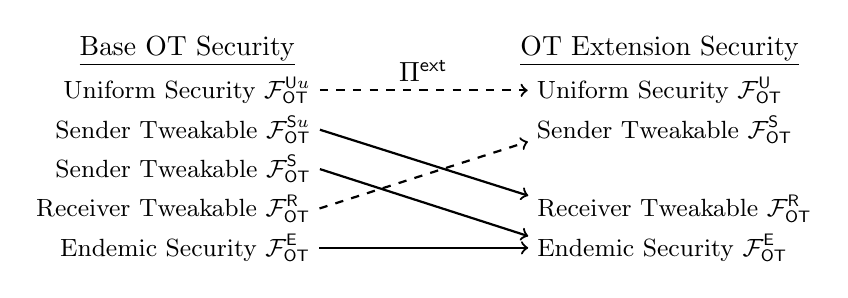
\begin{tikzpicture}[scale=0.5]\small
	\node (pi) at (6,4.5) {\normalsize $\Pi^\textsf{ext}$};
	\node (Base) at (0,5) {\underline{\normalsize Base OT Security}};
	\node (U) at (0,4) {Uniform Security $\OOT^{\U u}$};
	\node (SCu) at (-0.1,3) {Sender Tweakable $\OOT^{\send u}$};
	\node (SC) at (-0.1,2) {Sender Tweakable $\OOT^{\send}$};
	\node (RC) at (-0.35,1) {Receiver Tweakable  $\OOT^{\rec}$};
	\node (E) at (-0.05,0) {Endemic Security  $\OOT^{\E}$};
	
	
	\node (Ext) at (12,5) {\underline{\normalsize OT Extension Security}};
	\node (EU) at (12,4) {Uniform Security $\OOT^{\U}$};
	\node (ESC) at (12.13,3) {Sender Tweakable $\OOT^{\send}$};
	\node (ERC) at (12.38,1) {Receiver Tweakable  $\OOT^{\rec}$};
	\node (EE) at (12.07,0) {Endemic Security  $\OOT^{\E}$};
%	\draw [-implies,double equal sign distance] (U) -- (SC);
%	\draw [-implies,double equal sign distance] (U) -- (RC);
%	\draw [-implies,double equal sign distance] (SC) -- (E);
%	\draw [-implies,double equal sign distance] (RC) -- (E);
	\draw [->, thick, dashed] (U) -- (EU);
	\draw [->, thick] (E) -- (EE);
	\draw [->, thick] (SCu.east) -- (ERC.175);
	\draw [->, thick, dashed] (RC.east) -- (ESC.185);
	\draw [->, thick] (SC.east) -- (EE.175);
	
%	\draw [-, thick] (5,2.5)-- (TC);
%	\draw [->, thick] (E) .. controls (1,0.75) .. (SC);
%	\draw [->, thick] (E) .. controls (7,0.75) .. (RC);
	\end{tikzpicture}
	\label{fig:OTExtrelations}
	\caption{
		The figure depicts the implication different Base OT security notions (\definitionref{def:otSec}) have on the result OT extension protocol.  $A\rightarrow B$ denotes that any OT realizing security $A$ can be efficiently transformed by $\Pi^\textsf{ext}$ into an OT extension realizing security $B$, where $\Pi^\textsf{ext}$ is the protocol of \figureref{fig:otExt} such that $\OOT$ is the left hand side oracle. The dashed arrows are the same expect $\Pi^{\textsf{ext}}$ must be slightly modified. 
	}
\end{figure}










Next we review the OT extension protocol of \cite{RSA:OrrOrsSch17} which we describe in \figureref{fig:otExt}. The base OTs are performed on inputs that are sampled uniformly at random where the roles of the sender and receiver are reversed with respect to the OTs that are output by the extension. That is, \send will receiver $(b_j, \tt^j_{b_j})\in\mathbb{F}_2\times \mathbb{F}_2^m$ while $\rec$ will receive $(\tt^j_0,\tt^j_1)\in\mathbb{F}_2^m\times \mathbb{F}_2^m$ for $j\in[\nc]$.

\rec forms two matrices $T_0,T_1\in \mathbb{F}_2^{m\times \nc}$ by concatenating the base OT messages as column vectors, i.e. $T_i:=(\tt^1_i ... \tt^\nc_i)$. Similarly, \send forms the matrix $T_{\text{\textbf{b}}}:=(\tt^1_{b_1}...\tt^\nc_{b_\nc})$. \rec then encodes their 1-out-of-$N$ selections $\ww_1,...,\ww_m$ into a matrix $C\in \mathbb{F}_2^{m\times \nc}$. Each row $\cc_i$ is the codeword $\mathcal{C}(\ww_i)$ of \rec's $i$-th selection $\ww_i\in [N]$, $\mathcal{C}$ is a binary code of length $\nc$, dimension $\kc=\log_2\kappa$ and minimum distance $\dc\geq\kappa$. \rec sends the matrix
$$
	U=T_0+T_1+C
$$
to \send. Observe that $U$ encodes the selections of \rec but the selection is perfectly masked/encrypted due to the $j$-th column of $U$ being masked by the column $\tt^j_{1-b_j}$ which is uniformly distributed in the view of \send. Upon receiving $U$, \send computes $Q\in\mathbb{F}^{m\times\nc}$ where the $j$-th column is defined as $\qq^j:=b_j\cdot \uu^j+\tt^j_{b_j}=b_j\cdot \cc^j+\tt^j_0$. It holds that 
$$
	\qq_i=\cc_i\odot \bb + \tt_i
$$
where $\tt_i,\qq_i$ is the $i$-th row of $T_0,Q$, respectively, and $\bb:=(b_1,...,b_\nc)\in \mathbb{F}^\nc_2$. \rec will output $\vv_{i,\ww_i}:=\H(i, \tt_i)$. \send can then generate any OT message by computing $\vv_{i,\ww}:=\H(i, \qq_i + \mathcal{C}(\ww)\odot \bb)$. Correctness of this operation follows from 
\begin{align*}
	\qq_i + \mathcal{C}(\ww)\odot \bb =&  (\mathcal{C}(\ww_i)\odot \bb + \tt_i) + \mathcal{C}(\ww)\odot \bb\\
	=& (\mathcal{C}(\ww_i) + \mathcal{C}(\ww)) \odot \bb +\tt_i.
\end{align*}
Let $\delta = \mathcal{C}(\ww_i) + \mathcal{C}(\ww)$. In the event that $\ww_i=\ww$, then $\delta=0$ and \send computes the same $\vv_{i,\ww_i}$ value as \rec. Otherwise the hamming distance $\textsf{HD}(\delta)\geq \dc\geq \kappa$ by construction of $\mathcal{C}$. For $\rec$ to generate any other OT message $\vv_{i,\ww}$ s.t. $\ww\neq \ww_i$, \rec must guess the value $\delta\odot \bb\in \mathbb{F}^\nc_2$ given $\delta$, which takes time $2^{\textsf{HD}(\delta)}=O(2^\kappa)$.

To realize the ideal Sender Chosen Message oracle $\OOT^\send$ \cite{C:IKNP03,EC:ALSZ15,C:KelOrsSch15,RSA:OrrOrsSch17} specify two additional steps:
\begin{enumerate}

	\item A proof that all rows in $C$ can be decoded. Ishai et al. \cite{C:IKNP03} proposed a cut-and-choose approach while the more recent schemes \cite{C:KelOrsSch15,RSA:OrrOrsSch17} improve on the efficiency of these proofs by making \rec send random linear combinations of $\tt_i,\ww_i$ and having \send check they are consistent with same combination of $U$. We defer the details behind these proofs to \cite{C:KelOrsSch15,RSA:OrrOrsSch17}.
	
	\item The parties apply the Sender Chosen OT transformation $\Pi^{\send}_{1,N}$ from \figureref{fig:protoSendOT} which reduces sender chosen to endemic OT. That is, \send must send their chosen messages $(x_{i,1},...,x_{i,N})_{i\in [m]}$ encrypted under the corresponding key $(\vv_{i,1},...,\vv_{i,N})_{i\in [m]}$, e.g. \send sends $e_{i,j}:=x_{i,j}+\vv_{i,j}$ to \rec who outputs $x_{i,\ww_i}=e_{i,\ww_i}+\vv_{i,\ww_i}$. Note, this step is not included in \figureref{fig:otExt}. Next we will show without this step the protocol only achieves endemic security.
\end{enumerate}




\begin{figure}[t!]
	\vspace{-1cm}
	\framebox{\begin{minipage}{0.95\linewidth}\small
			\textsc{Parameters:} $\kappa$ is the computational security parameter. $m$ denotes the number of OTs. $N$ denotes the number of messages each OT has. $\mathcal{C}$ is an $[\nc,\kc,\dc]$ binary linear code such that $\kc=\log_2 N$ and $\dc\geq \kappa$. A bijective map $map : [N]\rightarrow\mathbb{F}^\kc$.\\
			\textsc{Requirements:} $\H : [m] \times \mathbb{F}_2^\nc \rightarrow \mathbb{F}_2^\kappa$ is a random oracle.			
			Let $m'=m+s$ where $s$ is defined in \stepref{step:consistency}. \OOT is an 1-out-of-2 OT oracle with output messages in $\mathbb{F}_2^{m'}$.
			\\
			
			\textsc{Extend:} On input $(\textsc{Extend})$ from \send and $(\textsc{Extend}, (x_1,...,x_m)\in[N]^m)$ from \rec.
			\begin{enumerate}
				\item\label{step:extInit} Both parties invoke $\nc$  instances of $\OOT$  where \send takes the role of the receiver. If $\OOT$ has inputs, the corresponding party  locally samples them uniformly from the input domains. \send receives $(\bb'\in\{1,2\}^\nc, \{\tt^j_{b_j}\}_{j\in [\nc]})$ where $\bb_i=(\bb_i'-1)\in\{0,1\}$. \rec receives $\{(\tt^j_0,\tt^j_1)\}_{j\in [\nc]}$. Let $T_0\in \mathbb{F}^{m'\times \nc}_2$ denote the matrix formed by concatenating the column vectors $\tt^1_0||...||\tt^\nc_0$. \\
				
				%				\item \rec constructs matrices $T_0,T_1\in \mathbb{F}^{m'\times \nc}_2$ from the seeds $\{(\rr^j_0,\rr^j_1)\}_{j\in [\nc]}$ so that the respective columns are:
				%				$$
				%					\tt^j_0 := \PRG(\rr^j_0)\in \mathbb{F}^{m'}_2,\qquad \tt^j_1 := \PRG(\rr^j_1)\in \mathbb{F}^{m'}_2,\qquad \forall j\in[\nc]
				%				$$
				%				In the same way \send produces $\tt^j_{b_j}$, for each $j\in[\nc]$. Summarizing, \rec holds $\{(\tt^j_0,\tt^j_1)\}_{j\in[\nc]}$ and \send holds $\{\tt^j_{b_j}\}_{j\in[\nc]}$.
				%				
				\item\label{step:extSendU} \rec  defines $\ww_i:=map(x_i)$ for $i\in[m]$ and  samples random $\ww_{m+\ell}\gets \mathbb{F}^\kc_2$, for $\ell\in[s]$. Then constructs a matrix $C\in\mathbb{F}^{m'\times \nc}_2$ such that each row $\cc_i$ is the codeword $\mathcal{C}(\ww_i)$. Then, \rec sends to \send the values
				$$
				\uu^j :=\tt^j_0 +\tt^j_1+\cc^j, \qquad \forall j\in[\nc],
				$$
				where $\cc^j$ is the $j$-th column of $C$.
				
				\item\label{step:extCompQ} \send receives $\uu^j\in\mathbb{F}^{m'}_2$ and computes
				$$
				\qq^j := b_j \cdot \uu^j +\tt^j_{b_j} = b_j\cdot \cc^j+\tt^j_0,\qquad \forall j\in[\nc]
				$$
				that form the columns of an $(m'\times \nc)$ matrix $Q$. Denoting the rows of $T_0, Q$ by $\tt_i,\qq_i$, \rec now holds $\cc_i,\tt_i$ and \send holds $\bb, \qq_i$ so that 
				$$
				\qq_i = \cc_i\odot \bb+\tt_i,\qquad \forall i\in[m'].
				$$
				
				\item \emph{Consistency check:}\label{step:consistency} \rec  proves in zero knowledge that given their view:
				\begin{center}
					$	\forall i\in[m], \exists w\in\mathbb{F}^\kc_2\  s.t.\  \cc_i \text{ decodes to } w \quad  \text{and}$ \\
					$\forall w'\in\mathbb{F}^\kc_2\setminus\{w\},$ the distribution of \\
					$(\cc_i+\mathcal{C}(w))\odot \bb$\\      
					has at least $\log_2(1/\negl)$ bits of entropy.
				\end{center}
				
				 For example, the proof of \cite{C:KelOrsSch15} for $N=2$ or \cite{RSA:OrrOrsSch17} otherwise. $s\geq0$ is specified by the proof protocol.
%				\begin{itemize}
%					\item Both parties query the challenge oracle $\O^{\textsf{chllng}}$ on input $u^j$ for $j\in[\nc]$  which samples and returns $X=\{(x_1^{\ell}, ...,x_m^{\ell} )\in \mathbb{F}^m_2\}_{\ell\in[s]}$ % := H'(\uu^1|| ... || \uu^\nc).
%					to both parties.
%					
%					\item \rec computes and sends, for $\ell \in[s]$:
%					$$
%					\widehat \tt^{\ell} := \sum_{i\in[m]} \tt_i \cdot x_i^\ell + \tt_{m+\ell}, \qquad \widehat \ww^\ell := \sum_{i\in[m]} \ww_i \cdot x_i^\ell + \ww_{m+\ell}
%					$$
%					
%					\item \send computes $\widehat \qq^\ell := \sum_{i\in[m]} \qq_i \cdot x^\ell_i + \qq_{m+\ell}$, and checks that:
%					$$
%					\widehat\tt^\ell + \widehat\qq^\ell = \mathcal{C}(\widehat\ww^\ell) \odot \bb, \qquad \forall\ell\in[s].
%					$$
%					If the check fails, \send sends $\textsf{Abort}$, and otherwise continues.
%				\end{itemize}
				\item \rec outputs $\vv_{i, x_j}:=\H(i,\tt_i)$ for all $i\in[m]$.
			\end{enumerate}
			
			
			\textsc{Output:} On input $(\textsc{Output}, (i,x))$ from \send. If $i\in[m],j\in[N]$, then \send outputs $\vv_{i,x}:=\H(i,\qq_i+\mathcal{C}(map(x))\odot \bb)$.
	\end{minipage}}
	\caption{ 1-out-of-$N$ OT Extension.}
	\label{fig:otExt}
\end{figure}


%\begin{figure}[t]
%	\framebox{\begin{minipage}{0.95\linewidth}\small
%			\textsc{Parameters:} $\lambda$ is the statistical security parameter.
%			
%			\textbf{Inputs:} \send inputs $U\in\mathbb{F}^{(m+\lambda)\times n}_2$ and \rec inputs $U'$.
%			\begin{enumerate}
%				\item \send uniformly samples $X\gets \mathbb{F}^{m\times n}_2$ and sends it to \rec.
%				\item Both parties output $X$.
%			\end{enumerate}
%	\end{minipage}}
%	\caption{ Challenge Protocol $\Pi^\textsf{chllng}$ implementing $\O^\textsf{chllng}$.}
%	\label{fig:OChallenge}
%\end{figure}


\subsection{OT Extension Attacks}

The authors of \cite{C:KelOrsSch15,RSA:OrrOrsSch17} provide protocol descriptions that are intended to satisfy the Uniform Message security notion, \definitionref{def:otSec}, but we show this to not be the case. For the rest of this work we will refer to the protocol of \cite{RSA:OrrOrsSch17} as defined in \definitionref{def:OOS} but note that the attacks on Uniform Message security also apply to \cite[Figure 6, 7]{C:KelOrsSch15}. In particular, we detail two attacks where the first (\lemmaref{lem:malRec})  allows a malicious \rec to bias the OT messages that they output while the second and third attacks (\lemmaref{lem:malRec}, \ref{lem:malSend}) succeed even when base OTs with stronger security are used. In all cases, the ability to bias the messages violates the ideal functionality which samples them uniformly at random.


\begin{definition}\label{def:OOS}
	Let $\Pi^{\textsf{OOS}}$ be the protocol of \figureref{fig:otExt} where $\OOT:=\OOT^\send$ (\definitionref{def:ot}), i.e.  \cite[Protocol 2]{RSA:OrrOrsSch17}.
\end{definition}
\begin{remark}\label{remark:oosROT}
	\cite{RSA:OrrOrsSch17} is inconsistent which type of base OTs should be used, switching between standard Sender Chosen Message OT ($\OOT^\send=\mathcal{F}^{\kappa,\nc}_{\textsf{2-OT}}$) in the protocol description, theorem statements and Uniform Message OT ($\OOT^\U=\mathcal{F}^{\kappa,\nc}_{\textsf{2-ROT}}$) in their proof. \lemmaref{lem:malRec} only applies to $\OOT^\send=\mathcal{F}^{\kappa,\nc}_{\textsf{2-OT}}$ while \lemmaref{lem:malRec2} and \ref{lem:malSend} apply even with $\OOT^\U=\mathcal{F}^{\kappa,\nc}_{\textsf{2-ROT}}$ base OTs. All three attacks apply to \cite{C:KelOrsSch15} which uses $\OOT^\send=\mathcal{F}^{\kappa,\nc}_{\textsf{2-OT}}$.
\end{remark}



\lemmaref{lem:malRec} details an attack which allows \R to bias the output $\vv_{i,x_i}$ to be $\H(i,x)$ for any $x\in\mathbb{F}^{\nc}_2$. The distinguisher compares the output of \send with $\vv_{i,x_i}$ and outputs 1 if they are equal. 


\begin{lemma} \label{lem:malRec}
	There exists a ppt adversary $\Adv$ and distinguisher $D$ such that for any $\Adv'$ 
	$$
	|\Pr[D((\send, \Adv)_{\langle\send, \Adv\rangle})=1]-\Pr[D((\O^{\U}_{\textsf{OT,\send}}, \Adv')_{\langle\OOT^\U, \Adv'\rangle})=1]|=1-2^{-\kappa}
	$$
	where $\langle\send, \Adv\rangle$ is the $\Pi^{\textsf{OOS}}$ protocol (\definitionref{def:OOS}), $\O^{\U}_{\textsf{OT,\send}}$ is the \send's side output within the view of $\OOT^{\U}$ and all algorithms additionally receive input $1^\kappa$. 
\end{lemma}
\begin{proof}
	For simplicity let $N=2$ and $m=1$. We define $\Adv$ as follows. $\Adv$ plays the role of \rec and replaces the input to base OTs, the sender input, with strings $\tt_0^j,\tt_1^j\in \{0\}^{m'}$ and then completes the protocol as normal.
	
	We define $D$ as follows. $D$ executes \send and \Adv with input $x_1=1$. \send outputs $(\vv_{1,1},\vv_{1,2})$ and $D$ outputs 1 if $\vv_{1,1}=\H(1, \{0\}^\nc)$ and 0 otherwise. In the real interaction it clearly holds that $\Pr[D((\send, \Adv)_{\langle\send, \Adv\rangle})=1]=1$. In the ideal interaction the honest \send will output a uniformly distributed $\vv_{1,1}\in\{0,1\}^\kappa$ which was sampled by $\OOT^{\U}$ and therefore $\Pr[D((\O^{\U}_{\textsf{OT,\send}}, \Adv')_{\langle\OOT^\U, \Adv'\rangle})=1]=2^{-\kappa}$.
\end{proof}



We now to our attention to a second class of adversary that can distinguish even when the base OTs output uniformly distributed messages, i.e. $\OOT^\U$. As \remarkref{remark:oosROT} indicates, the proofs contained in \cite{RSA:OrrOrsSch17} assume this base OT.

\begin{definition}\label{def:OOS2}
	Let $\Pi^{\textsf{OOS+}}$ be the protocol of \figureref{fig:otExt} where $\OOT:=\OOT^\U$ (\definitionref{def:ot}).
\end{definition}


The core idea behind this attack against $\Pi^{\textsf{OOS+}}$ is that \rec can choose their selection \emph{after} seeing what their output message is. This allows \rec to correlate their selection with their message and there by distinguish.

\begin{lemma} \label{lem:malRec2}
	There exists a ppt adversary $\Adv$ and distinguisher $D$ such that for any $\Adv'$ 
	$$
	|\Pr[D((\send, \Adv)_{\langle\send, \Adv\rangle})=1]-\Pr[D((\O^{\U}_{\textsf{OT,\send}}, \Adv')_{\langle\OOT^\U, \Adv'\rangle})=1]|=1-2^{-\kappa}
	$$
	where $\langle\send, \Adv\rangle$ is the $\Pi^{\textsf{OOS+}}$ protocol (\definitionref{def:OOS2}), $\O^{\U}_{\textsf{OT,\send}}$ is the \send's side output within the view of $\OOT^{\U}$ and all algorithms additionally receive input $1^\kappa$. 
\end{lemma}
\begin{proof}
	For simplicity let $N=2$ and $m=\kappa$. We define $\Adv$ as follows. $\Adv$ plays the role of \rec and receives the strings $\tt_0^j,\tt_1^j\in \{0\}^{m'}$ from \OOT. $\Adv$ redefines the selection values $x_1,...,x_m\in[2]$ of \rec such that $x_i:=\textsc{lsb}(\H(i, \tt_i))+1$. That is, $x_i$ equals the least significant bit of $\vv_{i,x_i}=\H(i, \tt_i)$ plus 1. \Adv executes the rest of the protocol as \rec would and outputs $(x_i)_{i\in [m]}$.
	
	We define $D$ as follows. $D$ executes \send and \Adv. \send outputs $(\vv_{i,1},\vv_{i,2})_{i\in[m]}$ and $D$ outputs 1 if $\forall i\in[m], \textsc{lsb}(\vv_{i,x_i})+1=x_i$ and 0 otherwise. In the real interaction it clearly holds that $\Pr[D((\send, \Adv)_{\langle\send, \Adv\rangle})=1]=1$. In the ideal interaction the honest \send will output a uniformly distributed $\vv_{i,1},\vv_{i,2}\in\{0,1\}^\kappa$ which are independent of $x_i$ and therefore $\Pr[D((\O^{\U}_{\textsf{OT,\send}}, \Adv')_{\langle\OOT^\U, \Adv'\rangle})=1]=2^{-\kappa}$.
\end{proof}



\lemmaref{lem:malSend} details another attack which performs an extension of size $m=\kappa$ and can distinguish the ideal oracle $\OOT^\U$ and $\Pi^{\textsf{OOS+}}$ with probability $1-2^m$. The core idea is that the malicious \send sets the base OT selection values to be $\mathbf{b}:=(1,...,1)\in [2]^\nc$. As such $\send$ learns the matrix $T_0$ in full. Recall that the output of \rec is defined to be the hash of the rows of $T_0$. Therefore \send can output the same message $\H(i, \tt_i)=\vv_{i,\ww_i}$ as \rec. For Sender Tweakable or Endemic security a viable simulation strategy is to extract $H(i, \tt_i)$ and define $\vv_{i,j}:=\H(i, \tt_i)$ for all $j$. However, there is no valid strategy for the Receiver Tweakable or Uniform Message security where the oracle samples some of the messages uniformly at random.

\begin{lemma} \label{lem:malSend}
	There exists a ppt adversary $\Adv$ and distinguisher $D$ such that for any $\Adv'$ 
	$$
		|\Pr[D((\Adv, \rec)_{\langle\Adv,\rec\rangle})=1]-\Pr[D((\Adv', \O^{\E}_{\textsf{OT,\rec}})_{\langle\Adv',\O^{\U}_{\textsf{OT}}\rangle})=1]|=1-\negl
	$$
	where $\langle\Adv,\rec\rangle$ is the $\Pi^{\textsf{OOS+}}$ protocol (\definitionref{def:OOS2}), $\O^{\E}_{\textsf{OT,\rec}}$ is the \rec's side output within the view of $\OOT^{\E}$ and all algorithms additionally receive input $1^\kappa$. 
\end{lemma}
\begin{proof} 
	For simplicity let $N=2$ and $m=\kappa$. We define $\Adv$ as follows. $\Adv$ plays the role of \send and replaces the input to $\OOT^\send$, the receiver input, with the string $\bb:=\{0\}^\nc$. \Adv outputs the matrix $Q$.
	
	We define $D$ as follows. $D$ samples the selection bits $x_1,...,x_m\gets[2]$ and sends them to \rec. $D$ executes $\Adv$ who outputs $Q$ and \rec outputs $\vv_{1,x_1},...,\vv_{m,x_m}$. If $\vv_{i,x_i}=\H(i,\qq_i)$ for all $i\in[m]$, output 1, otherwise 0. In the real interaction it clearly holds that $\Pr[D((\Adv, \rec)_{\langle\Adv,\rec\rangle})=1]=1$ since $\qq_i=\tt_i$.
	
	By definition the input of $\Adv'$ is independent of $x_i$ and receives no output from $\OOT^\E$ (apart from their input $(\vv_{0,i},\vv_{1,i})_{i\in [m]}$). Therefore, it must hold that $\Pr[D((\Adv', \rec)_{\langle\Adv',\O^{\E}_{\textsf{OT,\send}}\rangle})=1]=2^{\kappa}$.
\end{proof}





\subsection{OT Extension Security}


\begin{definition}\label{def:ext_E_E}
	Let $\Pi^{\textsf{ext-E}}$ be the protocol of \figureref{fig:otExt} where $\OOT:=\OOT^\E$ (\definitionref{def:ot}).
\end{definition}



\begin{lemma}\label{lem:ext-E}
	The $\Pi^{\textsf{ext-E}}$ protocol (\definitionref{def:ext_E_E}) is a 1-out-of-$N$ Oblivious Transfer ($\OOT^\E$) satisfying Endemic Message and Receiver Selection Security (\definitionref{def:otSec}).
\end{lemma}
\begin{proof}
	Correctness of the protocol was demonstrated by \cite{RSA:OrrOrsSch17}. The rest of the proof is essentially the same as \cite{RSA:OrrOrsSch17} except that the simulator extracts the messages from the malicious party.
	\begin{claim}[Malicious Sender Security]\label{claim:ext-E-MalSender}
		$\Pi^\textsf{ext-E}$ satisfies Security Against a Malicious Sender (\definitionref{def:otSec}) with respect to the $\OOT^\E$ oracle.
	\end{claim}
	\begin{proof}
		Consider the following hybrids which will define the simulator $\Adv'$. 
		\begin{enumerate}[leftmargin=1.8cm]
			\item[Hybrid 1.] $\Adv'$ internally runs \Adv while plays the role of $\rec$ and base OT oracle $\OOT=\OOT^\E$. For $j\in[\nc]$, $\Adv'$ receives $(\bb'_j,\tt^j_{\bb_j})\in [2]\times \mathbb{F}^{m'}_2$ from \Adv in \stepref{step:extInit} where $\bb_j:=\bb_j'-1$. $\Adv'$ uniformly samples $\tt^j_{1-\bb_j}$ as $\OOT=\OOT^\E$ would. $\Adv'$ sends $(\bb', \{\tt^j_{\bb}\})$ to $\Adv$ on behalf of \OOT. $\Adv'$ outputs whatever \Adv outputs. The view of $\Adv$ is unmodified.
			
			\item[Hybrid 2.] For \stepref{step:extSendU} $\Adv'$ does not sample $\tt^j_{1-\bb_j}$ and instead uniformly samples $U\gets\mathbb{F}^{m'\times \nc}_2$. $\Adv'$ sends $U$ to \Adv and then computes $Q$ as \send would. The view of $\Adv$ is identically distributed. This follows from the fact that $\tt^j_{1-\bb_j}$ is uniformly distributed in the view of \Adv and masks the $j$-th column of $U$ in the previous hybrid. 
			
			\item[Hybrid 3.]\label{hybrid:malSendExtract} For each row $\qq_i$, $\Adv'$ defines the circuit $\mathcal{M}_i:[N]\rightarrow\{0,1\}^\kappa$ such that on input $j\in[N]$ it outputs $\H(i, \qq_i+\bb\odot \mathcal{C}(map(j)))$. $\Adv'$ sends $\mathcal{M}_i$ to the ideal oracle $\OOT^\E$ as the sender's input to the $i$-th OT instance. This change allows the ideal oracle to output the same distribution as the real protocol. The view of $\Adv$ is unmodified.
			
			Note, $\Adv$ can influence $\mathcal{M}_i(j)=\H(i, \qq_i+\bb\odot \mathcal{C}(map(j)))=H(i, (c_i + \mathcal{C}(map(j)) \odot \bb + \tt_i)$ by choosing $\bb$ and the bits $\{\tt_i[j] \mid \bb_j=0\}$.
			
			\item[Hybrid 4.] For \stepref{step:consistency} $\Adv'$ simulates the consistency proof. This change is indistinguishable. 
			
			\item[Hybrid 5.] $\Adv'$ does not take the input of \rec. \rec only interacts with $\OOT^\E$. This change is identically distributed since $\Adv'$ was not using the input of \rec.
		\end{enumerate}
	\end{proof}

	\begin{claim}[Malicious Receiver Security]\label{claim:ext-E-MalReceiver}
	$\Pi^\textsf{ext-E}$ satisfies Security Against a Malicious Receiver (\definitionref{def:otSec}) with respect to the $\OOT^\E$ oracle.
	\end{claim}
	\begin{proof}
				Consider the following hybrids which will define the simulator $\Adv'$. 
		\begin{enumerate}[leftmargin=1.8cm]
			\item[Hybrid 1.] $\Adv'$ internally runs \Adv while plays the role of $\send$ and base OT oracle $\OOT=\OOT^\send$. $\Adv'$ receives $\{\tt^j_0,\tt^j_1\}_{i\in\nc}$ from \Adv in \stepref{step:extInit} and samples $\bb$ as \send would. $\Adv'$ outputs whatever \Adv outputs. The view of $\Adv$ is unmodified.
			
			\item[Hybrid 2.] In \stepref{step:extSendU} $\Adv'$ receives $U$ from $\Adv$.  $\Adv'$ computes $C$ and $Q$ using $\tt_0^j,\tt_1^j,\bb$. $\Adv'$ performs the proof of \stepref{step:consistency} as \send would. If the proof fails, $\Adv'$ aborts as \send would. Otherwise, by the correctness of the proof, $\cc_i$ decodes to $\ww_i$.
			
			$\Adv'$ defines the circuit $\mathcal{S}_i$ with support $\{\ww_i\}$ and $\mathcal{M}_i:[1]\rightarrow\mathbb{F}^\kappa_2$ s.t. $\mathcal{M}_i(1)=\H(i, \tt_i)$. $\Adv'$ sends $\mathcal{S}_i$ and $\mathcal{M}_i$ to $\OOT^\E$ as the receiver's input to the $i$-th OT instance. The view of \Adv is unmodified and the ideal and real output agree on output $\vv_{i,x_i}$.
			
			\item[Hybrid 3.]\label{hybrid:simOutput} Assuming $\Adv'$ did not abort in \stepref{step:consistency}, for all $w\neq \ww_i$, \rec has $\negl$ probability of computing $g=\qq_i+\bb\odot \mathcal{C}(w)$. If this was not the case, then \rec could compute
			\begin{align*}
			g +\tt_i &=\qq_i+\bb\odot \mathcal{C}(w)+\tt_i\\
			&=\cc_i\odot\bb+\tt_i+\bb\odot \mathcal{C}(w)+\tt_i\\
			&=(\cc_i+\mathcal{C}(w))\odot \bb
			\end{align*}
			which contradicts the proof of \stepref{step:consistency}.
			Therefore, the probability that \Adv has made a query of the form $\H(i,\qq_i+\bb\odot \mathcal{C}(w))$ for $w\neq \ww_i$ is also negligible. If such as query does happen $\Adv'$ aborts. Otherwise, if \send makes an $\H$ query of the form $\H(i,\qq_i+\bb\odot \mathcal{C}(w))$ for a new $(i,w)$ pair and $w\neq \ww_i$, then $\Adv'$ computes $x$ s.t. $map(x)=w$ and sends $(\textsc{Output}, x)$ to the $i$-th instance of $\OOT^E$ and receives $\vv_{i,x}\gets\{0,1\}^\ell$ in response. $\Adv'$ programs $\H$ to output $\vv_{i,x}$ on this query. All other $\H$ queries are answered as normal. The distribution of $\H$ after being programmed is identical since the input has not previously been queried and in both cases the result is uniformly distributed. This hybrid is indistinguishably distributed from the previous. In particular, $\Adv'$ may now abort on bad $\H$ queries made by \rec which happens with $\negl$ probability.
			
			\item[Hybrid 4.] $\Adv'$ does not take the input of \send and does not program $\H$ in \hybridref{hybrid:simOutput}. \send only interacts with $\OOT^\E$. This change is identically distributed.
		\end{enumerate}
	\end{proof}
\end{proof}



\begin{definition}\label{def:ext_S_U}
	Let $\Pi^{\textsf{ext-S}}$ be the protocol of \figureref{fig:otExt} where $\OOT:=\OOT^\send$.
\end{definition}
\begin{lemma}
	The $\Pi^\textsf{ext-S}$ protocol realizes 1-out-of-$N$ $\OOT^\E$ security.
\end{lemma}
\begin{proof}
	Follows directly from \lemmaref{lemma:is_a} and \lemmaref{lem:ext-E}.
\end{proof}
\begin{lemma}
		The $\Pi^\textsf{ext-S}$ protocol does not realizes 1-out-of-$N$ $\OOT^\send$ or $\OOT^\rec$ security.
\end{lemma}
\begin{proof}
	Follows directly from \lemmaref{lemma:is_a} with \lemmaref{lem:malRec2} for $\OOT^\send$ and \ref{lem:malSend} for $\OOT^\rec$.
\end{proof}



\begin{definition}\label{def:ext_Su_R}
	Let $\Pi^{\textsf{ext-S}u}$ be the protocol of \figureref{fig:otExt} where $\OOT:=\OOT^{\send u}$.
\end{definition}
\begin{lemma}
	The $\Pi^{\textsf{ext-S}u}$ protocol realizes 1-out-of-$N$ $\OOT^\rec$ security.
\end{lemma}
\begin{proof}
	Security against a malicious receiver follows from \lemmaref{lemma:is_a} and \lemmaref{lem:ext-E}. 
	
	
	\begin{claim}[Malicious Sender Security]\label{claim:ext-Su-MalSender}
		$\Pi^\textsf{ext-E}$ satisfies Security Against a Malicious Sender (\definitionref{def:otSec}) with respect to the $\OOT^\rec$ oracle.
	\end{claim}
	\begin{proof}
		Observe that the honest receiver uniformly chooses
	\end{proof}
\end{proof}




%\section{Optimality of the Result}

\newcommand{\OG}{\ensuremath{\O_{\mathsf{G}}}\xspace}
\newcommand{\OK}{\ensuremath{\O_{\mathsf{K}}}\xspace}
\newcommand{\sk}{\ensuremath{\mathsf{sk}}\xspace}
\newcommand{\pk}{\ensuremath{\mathsf{pk}}\xspace}
\renewcommand{\L}{\ensuremath{\mathsf{L}}\xspace}
\newcommand{\LOG}{\ensuremath{\L_{\OG}}\xspace}
\newcommand{\LOK}{\ensuremath{\L_{\OK}}\xspace}
\newcommand{\E}{\ensuremath{\mathsf{E}}\xspace}



\begin{definition}[Asymmetric Random Oracle]
An \emph{asymmetric random oracle} consists of two oracles \OG and \OK, with the following description.
\begin{description}
\item[\OG:] \OG has a list \LOG that is empty in the beginning. On an (empty) query, \OG samples $\sk\leftarrow\bits^{\sec}$. If $(\sk,*)\not\in\LOG$, it samples  $\pk\leftarrow\bits^{\sec}$. Then it outputs and stores  $(\sk,\pk)$ in \LOG. If $(\sk,*)\in\LOG$, \OG outputs entry $(\sk,\pk)$ of \LOG.
\item[\OK:] \OK has a list \LOK, which is empty in the beginning, and access to list \LOG. On a query $(\sk_1,\pk_2)$, \OK looks up $\pk_1$ s.t. $(\sk_1,\pk_1)\in\LOG$. If $(\pk_1,\pk_2,\key)$ or $(\pk_2,\pk_1,\key)$ are in \LOK, it outputs $\key$. Otherwise it samples $\key\leftarrow\bits^{\sec}$, outputs $\key$ and stores $(\pk_1,\pk_2,\key)$ in \LOK.  
\end{description} 
\end{definition}

\begin{lemma}
Let $\langle \A, \B\rangle$ be a protocol between two parties \A and \B with access to a random oracle \H and an asymmetric random oracle $(\OG, \OK)$, where the outputs of \OK are submitted to \A, \B after all messages are sent. Then, there is an algorithm \E that takes as input the transcript $\langle \A, \B\rangle$ and outputs two lists $\L_1, \L_2$, such that with high probability, the views of \A and \B are mutually independent conditioned on $\L_1$, $\L_2$, transcript $\langle \A, \B\rangle$ and $(\pk_{\A,i},\pk_{\B,j},\key)_{i\in[Q_{\A}],j\in[Q_{\B}]}\subseteq\LOK$.
\end{lemma}

\begin{lemma}
Let $\langle \A, \B\rangle$ be a protocol between two parties \A and \B with access to a random oracle \H and an asymmetric random oracle $(\OG, \OK)$, where \A makes $Q_{\A}$ and \B $Q_{\B}$ queries to $\OG$. Then, there is an algorithm \E that takes as input the transcript $\langle \A, \B\rangle$, the $Q_{\A}\cdot Q_{\B}$ asymmetric intersection queries $(\pk_{\A,i},\pk_{\B,j},\key)_{i\in[Q_{\A}],j\in[Q_{\B}]}\subseteq\LOK$ and outputs two lists $\L_1, \L_2$, such that with high probability, the views of \A and \B are mutually independent conditioned on $\L_1$, $\L_2$, transcript $\langle \A, \B\rangle$ and $(\pk_{\A,i},\pk_{\B,j},\key)_{i\in[Q_{\A}],j\in[Q_{\B}]}\subseteq\LOK$.
\end{lemma}



\begin{theorem}
There is no secure $k$ out of $n$ endemic OT where the sender makes at most $n$ queries to $\OK$ and the receiver makes at most $k-1$ queries to $\OG$. 
\end{theorem}

\begin{proof}
We show that there is either a sucessful malicious sender or receiver that breaks the protocol. We start by constructing a malicious sender that receives $k-1$ OT strings learned by the receiver and tries to determine the $k$-th OT string. An attack that is successful with more than probability $\frac{1}{n-k-1}$ would violate the security of the OT. 

On a high level, the malicious sender chooses the following strategy. It runs the normal protocol interacting with \rec to receive the OT strings $(s_i)_{i\in[n]}$. Further, \rec sends him $k-1$ of his learned strings $(s_i)_{i\in\set_1}$, where $\set_1$ has size $k-1$. It will then run algorithm \E to learn the two lists $\L_1$, $\L_2$, where it provides \E his own list of query answer pairs of $\OK$, which contains all asymmetric intersection queries. 

Now, given the transcript, $L_1$, $L_2$ the views of the malicious sender and \rec are mutually independent. This allows the malicious sender to resample the view of \rec such that its output, $(s_{\rec,i})_{i\in\set_{\rec}}$, where $\set_{\rec}$ has size $k$, is still consistent with its own view, i.e. $(s_{\rec,i})_{i\in\set_{\rec}}\subset(s_i)_{i\in[n]}$. The malicious sender uses this resampling procedure to determine 
\end{proof} 
\section{Implementation}\label{sec:impl}

We implement and benchmark several variants of our OT protocols. 





\newcommand{\PreserveBackslash}[1]{\let\temp=\\#1\let\\=\temp}
\newcolumntype{C}[1]{>{\PreserveBackslash\centering}p{#1}}
\newcolumntype{R}[1]{>{\PreserveBackslash\raggedleft}p{#1}}
\newcolumntype{L}[1]{>{\PreserveBackslash\raggedright}p{#1}}

\begin{figure*}[t!]\centering
	\begin{tabular}{|c||c|c || r | r|  r | r |r |r|r |r|}
		\hline
		\multirow{3}{*}{Protocol} & \multirow{3}{*}{Security}           & \multirow{3}{*}{Rounds} &                             \multicolumn{8}{c|}{$m$}                              \\
		                          &                                     &                         & 1      & 32     & 128     & 512       & 1        & 32       &      128 & 512      \\ \cline{4-11}
		                          &                                     &                         &       \multicolumn{4}{c|}{LAN}       &         \multicolumn{4}{c|}{WAN}          \\ \hline\hline
		   \cite{LC:ChoOrl15}     & GapDH, RO$\rightarrow$ ``Random OT" & 2                       & 5      & 70     & 230     & 662       & 106      & 200      &      365 & 785      \\ \hline
		  \cite{SODA:NaoPin01}    & DDH, RO $\rightarrow\OOT^\send$     & 3                       & 5      & 67     & 203     & 573       & 155      & 185      &      304 & 593      \\ \hline
		          This            & DDH, RO $\rightarrow\OOT^\E$        & 1                       & 3      & 46     & 148     & 480       & {\bf 54} & 135      &      240 & 570      \\ \hline
		          This            & LWE, RO $\rightarrow\OOT^\send$ or $\OOT^{\send u}$    & 2                       & {\bf1} & {\bf6} & {\bf24} & {\bf 105} & 101      & {\bf115} & {\bf154} & {\bf481} \\ \hline
	\end{tabular}
	\caption{ \label{fig:baseTimes}}	
\end{figure*}



\begin{figure*}[t!]\centering
	\begin{tabular}{|c||c|c|c || r | r|  r |r |r|r |r|r|}
		\hline
		\multirow{3}{*}{Protocol} &         \multirow{3}{*}{Security}          & \multirow{3}{*}{Total} & \multirow{3}{*}{$n$} &                                     \multicolumn{8}{c|}{$m$}                                     \\
		                          &                                            &                         &                      & $2^{12}$ & $2^{16}$ & $2^{20}$ & $2^{24}$  & $2^{12}$  &  $2^{16}$ & $2^{20}$    &      $2^{24}$ \\ \cline{5-12}
		                          &                                            &          Rounds         &                      &          \multicolumn{4}{c|}{LAN}          &              \multicolumn{4}{c|}{WAN}               \\ \hline\hline
		                          &  $\OOT^{\send u},$RO $\rightarrow\OOT^\U$  &            4            &       $2^{76}$       & 20       & 151      & 1,612    & 24,060    & 345       &       833 & 7003        &       103,481 \\ \hline
		 $\Pi^{\textsf{ext-S}u}$  & $\OOT^{\send u},$RO $\rightarrow\OOT^\rec$ &         {\bf 2}         &          2           & 14       & 76       & 610      & 8,224     & 406       &       700 & 6,488       &        32,315 \\ \hline
		$\Pi^{\textsf{ext-S}u+}$  &  $\OOT^{\send u},$RO $\rightarrow\OOT^\U$  &            4            &          2           & 18       & 70       & 547      & 7,429     & 407       &       708 & 2,666       &        32,856 \\ \hline
		 $\Pi^{\textsf{ext-S}u}$  &  $\OOT^{\U u},$IC $\rightarrow\OOT^\rec$   &         {\bf 2}         &          2           & 14       & 22       & 174      & 1,158     & {\bf 300} & {\bf 530} & {\bf 2,097} & {\bf  25,701} \\ \hline
		 $\Pi^{\textsf{ext-U}u}$   &   $\OOT^{\U u},$IC $\rightarrow\OOT^\U$    &           4            &          2           & {\bf6}   & {\bf24}  & {\bf101} & {\bf 720} & {395}     &    { 645} & {2,128}     &      {26,256} \\ \hline
	\end{tabular}
	\caption{ \label{fig:extTimes}}	
\end{figure*}






\bibliographystyle{alpha}
\bibliography{bib,cryptobib/abbrev3,cryptobib/crypto}

\appendix
\section{Additional Preliminary Definitions and Lemmata}\label{sec:defsandlems}



\begin{definition}[Coin Tossing]\label{def:coin}
An \emph{ideal coin tossing} is a functionality denoted with $\F^{\coin}$ that interacts with two parties \A and \B, samples a uniform string $r\in\bits^*$ and sends $r$ to $\A$ and $\B$.
\end{definition}

\newcommand{\extract}{\ensuremath{\mathsf{ext}}\xspace}

\begin{definition}[Extractable Commitments]\label{def:com}
An \emph{extractable commitment scheme} consists of three algorithms.
\begin{description}
\item[$\com(x,r)$:] Commits to $x$ using randomness $r$. 
\item[$\open(\com,x,r)$:] Outputs $1$ if commitment $\com\in\com(x,r)$.
\item[$\extract(\com,\aux)$:] Given some auxiliary information, it extracts committed value $x$. 
\end{description}
For security, we ask that it is hiding, i.e. for any $x,m$, $x, \com(x,r)$ is indistinguishable from $m,\com(x,r)$ and that it is binding, i.e. for any $x$, $\extract(\com(x,r))$ outputs $x$.
\end{definition}

An extractable commitment can easily constructed using a random oracle by defining $\com(x,r):=H(x,r)$, $\open$ simply evaluates $\H$ and checks equality and the $\extract$ algorithm observes the random oracle queries from which $x$ can be learned.

\subsection{Key Agreement}\label{sec:addKA}
We give the following additional security definition for key agreement protocols.

\begin{definition}[One-Round Uniform Key Agreement]
We call a \UKA \emph{one-round uniform key agreement} if the function $\mes_{\B}\leftarrow\B(\tape_{\B},\mes_\A)$ does not depend on $\mes_A$ and can be computed solely using input $\tape_{\B}$. More precisely, there is a function $\B'$ such that for any $\mes_{\A}$, $\B'(\tape_{\B})=\B(\tape_{\B},\mes_{\A})$, which we will in the following refer to with $\B$ as well. 
\end{definition}

\begin{definition}[Multi-Instance Uniformity]
We call a \UKA $Q$ \emph{multi-instance uniform} if for any ppt distinguisher \D and any polynomial size auxiliary input $z$,
$$
|\Pr[\D^{\O_{\A}}(z)]=1]-Pr[\D^{\O_{u}}(z)=1]|=\negl,
$$
where $\O_{\A}$ outputs $\mes_\A\leftarrow\A(\tape_\A)$ for fresh randomness $\tape_\A$ and $\O_u$ outputs $u\leftarrow\G$ and $Q$ is a bound on the amount of queries to $\O_{u}$, $\O_{\A}$.
\end{definition}



\begin{definition}[Multi-Instance Key Indistinguishability]
We call a \UKA $(Q,n)$ \emph{multi-instance key indistinguishable} if for any ppt distinguisher \D and any polynomial size auxiliary input $z$,
$$
|\Pr[\D^{\O_{\langle \A,\B\rangle}, \O_{\key}}(z)]=1]-Pr[\D^{\O_{\langle \A,\B\rangle},\O_{u}}(z)=1]|=\negl,
$$
where $\O_{\langle \A,\B\rangle}$ outputs on the $i$-th query a transcript $\T_i:=\langle \A_i,\B_i\rangle$, $\O_{\key}$ outputs on query $j$, key $\key_j=\EK(\tape_{\A,j},\mes_{\B,j})=\EK(\tape_{\B,j},\mes_{\A,j})$ that matches transcript $\T_i$. $\O_u$ outputs a uniform element $u$ from the key domain. $\O_{\langle \A,\B\rangle}$ uses fresh random tapes $\tape_{\A,i},\tape_{\B,i}\leftarrow\bits^*$ for every query. $Q$ is a bound on the amount of queries to $\O_{\langle \A,\B\rangle}$, where $n$ bounds the amount of queries to $\O_{\key}$, $\O_{u}$. 
\end{definition}

In case of a one-round \UKA, we define a stronger version of the multi-instance key indistinguishability, which we call one-round multi-instance key indistinguishability.

\begin{definition}[One Round Multi-Instance Key Indistinguishability]
We call a one-round \UKA $(Q,n)$ \emph{one-round multi-instance key indistinguishability} if for any ppt distinguisher \D and any polynomial size auxiliary input $z$,
$$
|\Pr[\D^{\O_{\A}, \O_{\key}}(z,\mes_\B)]=1]-Pr[\D^{\O_{\A},\O_{u}}(z,\mes_\B)=1]|=\negl,
$$
where $\mes_{\B}\leftarrow\B(\tape_{\B})$ for uniform $\tape_{\B}$. $\O_{\A}$ outputs on the $i$-th query $\mes_{\A,i}\leftarrow \A(\tape_{\A,i})$ for uniform $\tape_{\A,i}$. $\O_{\key}$ outputs on query $j$, key $\key_j=\EK(\tape_{\A,j},\mes_{\B})=\EK(\tape_{\B},\mes_{\A})$. $\O_u$ outputs a uniform element $u$ from the key domain. $Q$ is a bound on the amount of queries to $\O_{\A}$, where $n$ bounds the amount of queries to $\O_{\key}$, $\O_{u}$. 
\end{definition}

In the next lemmata, we show that all the security notions are implied by the standard definitions, but potentially with a polynomial security loss.
 
\begin{lemma}\label{lem:multuniform}
Let \UKA be uniform except probability $\epsilon$, then it is $Q$ multi-instance uniform except at most probability $Q\epsilon$.
\end{lemma}
\begin{proof}
This follows straightforwardly from using a simple hybrid argument. Hybrid $\hyb_{i}$ samples $\mes_{\A,j}$ for $j\leq i$ from $\O_u$ and for $j>i$ from $\O_{\A}$. If there is an adversary that distinguishes $\hyb_i$ from $\hyb_{i+1}$ for any $i$, then we can break the uniformity of \UKA by distinguishing $\mes_{\A,i+1}$ from uniform.  
\pe
\end{proof}

\begin{lemma}\label{lem:keytomultkey}
Let \UKA be key indistinguishable except probability $\epsilon$, then it is $(Q,n)$ multi-instance key indistinguishable except at most probability $Q\epsilon$. 
\end{lemma}

\begin{proof}
Again, we use a hybrid argument over hybrids $\hyb_i$. In $\hyb_i$, $(\mes_{\A,j},\mes_{\B,j}),\key_j$ is sampled from $\O_{\langle \A,\B\rangle}\times\O_u$ for $j\leq i$ and from $\O_{\langle \A,\B\rangle}\times\O_\key$ for $j>i$. If one distinguishes $\hyb_i$ from $\hyb_{i+1}$ for some $i$, one breaks the key indistinguishability. 
\pe
\end{proof}

\begin{lemma}\label{lem:oneroundkeytomultkey}
Let a one-round \UKA be key indistinguishable except probability $\epsilon$, then it is $(Q,n)$ one-round multi-instance key indistinguishable except at most probability $Q\epsilon$. 
\end{lemma}

\begin{proof}
This lemma follows for the same reason as \lemmaref{lem:keytomultkey}.
\pe
\end{proof}


\subsection{Oblivious Transfer}\label{sec:addOT}


\begin{lemma}[Repeat of \lemmaref{lemma:is_a}]\label{lemma:is_a_repeat}
	Let the distribution of OT strings be efficiently sampleable. 
	Then $\OOT^\U$-security implies $\OOT^{\send}$ as well as $\OOT^\rec$-security. $\OOT^{\send}$ or $\OOT^\rec$-security imply $\OOT^\E$-security.
\end{lemma}

\begin{proof}
	In the first step, we show that uniform message security implies sender chosen message security and receiver chosen message security implies endemic security. These two implications result from the same simple fact that a malicious sender interacting with the ideal OT is easier to construct when it can choose the OT strings than when it receives the strings from the ideal OT. The following claim formalizes this fact. 
	\begin{claim}\label{claim:utocs}
		Let $\Pi$ be an OT secure against a malicious sender with respect to an ideal OT $\OOT^*$ that sends the OT strings $(s_i)_{i\in[n]}$ to the sender, i.e. functionality $\OOT^\U$ and $\OOT^{\rec}$, and the distribution of $(s_i)_{i\in[n]}$ is efficiently sampleable. Then $\Pi$ is also secure against a malicious sender with respect to ideal OT $\OOT$, which receives the OT strings $(s_i)_{i\in[n]}$ from the sender, i.e functionality $\OOT^\send$ and $\OOT^\E$.
	\end{claim}
	
	
	\begin{proof}
		We show that if there is an adversary that breaks the security against a malicious security with respect to ideal OT $\OOT$ then there is also an adversary that breaks the security with respect to $\OOT^*$. More precisely, if there is a ppt adversary $\Adv_1$ such that for any ppt adversary $\Adv_1'$ there exists a ppt distinguisher $\D_1$ with 
		$$
		|\Pr[\D_1((\Adv_1,\rec)_{\Pi})=1] -\Pr[\D_1( (\Adv'_1, \OOT))=1]|=\epsilon,
		$$
		where all algorithms receive input $1^\sec$ and \rec additionally receives input \set.
		Then there is also a ppt adversary $\Adv_2$ such that for any ppt adversary $\Adv_2'$ there exists a ppt distinguisher $\D_2$ with 
		$$
		|\Pr[\D_2((\Adv_2,\rec)_{\Pi})=1] -\Pr[\D_1( (\Adv'_2, \OOT^*))=1]|=\epsilon,
		$$
		where all algorithms receive input $1^\sec$ and \rec additionally receives input \set.
		
		We set $\Adv_2:=\Adv_1$ and $\D_2:=\D_1$. Further, for any $\Adv_2'$, there is an $\Adv_1'$  such that the distribution of $(\Adv'_2, \OOT^*)$ is identical with the distribution $(\Adv'_1, \OOT)$. This follows from the fact that  $\Adv_1'$ could choose the OT strings $(s_i)_{i\in[n]}$  from the same distribution as $\OOT^*$ does and otherwise follow the description of $\Adv_2'$. Since $\D_1$ is successful for any $\Adv_1'$ it will be also for any $\Adv_2'$, which can be seen as a subset of the set of all ppt adversaries $\Adv_1'$.
		\pe
	\end{proof}
	
	The remaining two implications, from uniform security to receiver chosen message security and from sender chosen message security to endemic security follow in a similar fashion. Again it is easier to construct a malicious receiver interacting with the ideal OT when he can choose the OT strings rather than receiving them from the ideal OT.
	\begin{claim}\label{claim:utocr}
		Let $\Pi$ be an OT secure against a malicious receiver with respect to an ideal OT $\OOT^*$ that sends the learned OT strings $(s_i)_{i\in\set}$ to the receiver, i.e. functionality $\OOT^\U$ and $\OOT^{\send}$, and the distribution of $(s_i)_{i\in\set}$ is efficiently sampleable. Then $\Pi$ is also secure against a malicious sender with respect to ideal OT $\OOT$, which receives the OT strings $(s_i)_{i\in\set}$ from the receiver, i.e. $\OOT^\rec$ and $\OOT^\E$.
	\end{claim}
	
	\begin{proof}
		The proof is basically identical to the proof of Claim~\ref{claim:utocs}. Again, the set of all ppt $\Adv_2'$ is a subset of the set of all ppt $\Adv_1'$ and identical with the set of all $\Adv_1'$ that sample  $(s_i)_{i\in\set}$ from the same distribution as when sent by $\OOT^*$.
		\pe
	\end{proof}
	\pe
\end{proof}



In the following, we give a generalized definition of OT.

\begin{definition}[Generalize Ideal $k$-out-of-$n$ Oblivious Transfer]\label{def:got}
	A (generalized) \emph{ideal $k$-out-of-$n$ oblivious transfer} is a functionality that interacts with two parties, a sender \send and a receiver \rec. Let $\set\subseteq[n]$ of size $k$ and  $s_1,...,s_n\in \{0,1\}^\ell$.
	
	The functionality is publicly parameterized by one of the following message sampling methods:
	\begin{description}
		\item[] \textsc{Sender Chosen Message:} $\send$ sends the circuit $\mathcal{M} : [n] \rightarrow \{0,1\}^\ell$ to the functionality which defines $s_i:=\mathcal{M}(i)$.
		
		\item[] \textsc{Receiver Chosen Message:} \rec sends the circuit  $\mathcal{M} : [k] \rightarrow \{0,1\}^\ell$ to the functionality which defines $s_{\set_i}:=\mathcal{M}(i)$ for $i\in[k]$ and uniformly samples $s_i\gets\{0,1\}^\ell$ for $i\in\set\setminus[n]$.
		
		\item[] \textsc{Uniform Message:} The functionality uniformly samples $s_i\gets\{0,1\}^{\ell}$ for $i\in[n]$. 
		
		\item[] \textsc{Endemic:} If $\send$ is corrupt, then $\send$ sends the circuit $\mathcal{M} : [n] \rightarrow \{0,1\}^\ell$ to the functionality which defines $s_i:=\mathcal{M}(i)$.
		
		If \rec is corrupt, \rec sends the circuit  $\mathcal{M} : [k] \rightarrow \{0,1\}^\ell$ to the functionality which defines $s_{\set_i}:=\mathcal{M}(i)$ for $i\in[k]$.
		
		All remaining $s_i$ for $i\in [n]$ are uniformly samples $s_i\gets\{0,1\}^\ell$.
	\end{description}
	
	The functionality is publicly parameterized by one of the following selection methods:
	\begin{description}
		\item[] \textsc{Receiver Selection:} \rec sends the circuit $\mathcal{S}:[n]\rightarrow\{0,1\}$ to the functionality where the support of $\mathcal{S}$ is of size $k$. The functionality defines $\set:=\{i \mid \mathcal{S}(i)=1\}$.
		\item[] \textsc{Uniform Selection:} The functionality uniformly samples $\set\gets\mathbb{P}([n])$ s.t. $|\set|=k$.
	\end{description}
	
	As specified by the message sampling method, the oracle receives the circuit $\mathcal{M}$ from the appropriate party if one is called for.  As specified by the selection method, the functionality receives the circuit $\mathcal{S}$ if one is called for. 
	Thereafter, upon receiving the message $(\textsc{Output}, i)$ from \send, respond with $s_i$. Upon receiving $(\textsc{Output}, i)$ from \rec and if $i\in \set$,  respond with $s_i$. 
	
	We denote the ideal functionalities for sender chosen, receiver chosen, uniform and endemic with receiver selection as $\OOT^\send, \OOT^\rec,\OOT^\U,\OOT^\E$, respectively. The analogous oracles for Uniform Selection are denoted as  $\OOT^{\send u},$ $\OOT^{\rec u}, \OOT^{\U u}, \OOT^{\E u}$, respectively.
\end{definition}
\begin{remark}
	When $n$ is polynomial in the security parameter $\kappa$, we simplify the above definition to \definitionref{def:ot} to allow the parties directly input the appropriate $s_i$ messages as opposed to specifying a circuit $\mathcal{M}$. Similarly for the set $\set:=\{i \mid \mathcal{S}(i)=1\}$. Lastly, instead of querying the oracle with $(\textsc{Output}, i)$, the oracle sends $(s_i)_{i\in [n]}$ to \send and $(\set, (s_i)_{i\in\set})$ to \rec. This simplification can trivially be simulated when $n=\textsf{poly}(\kappa)$.
\end{remark}


The following transformation allows to transform an OT where the receiver's choice bit is chosen to an OT with a random choice bit. This transformation is very useful in the context of OT extension.

\begin{figure}
\centering
\framebox{
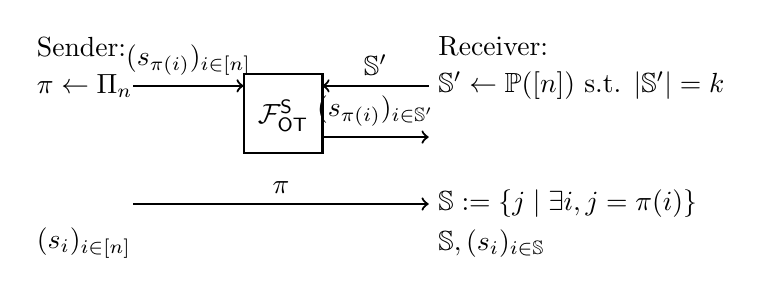
\begin{tikzpicture}
\node [anchor=west] at (0,5) {Sender:};
\node [anchor=west] at (5.1,5) {Receiver:};
\begin{scope}[shift={(-2,0)}]
\draw [thick] (4.75,4.65)--(5.75,4.65)--(5.75,3.65)--(4.75,3.65)--cycle;
\node at (5.25,4.125){$\OOT^\send$};
\draw [thick, <-] (5.75,4.5)-- node [midway,above]{$\set'$}(7.1,4.5);
\draw [thick, ->] (5.75,3.85)-- node [midway,above]{$(s_{\pi(i)})_{i\in \set'}$}(7.1,3.85);
\draw [thick, ->] (3.35,3)-- node [midway, above]{$\pi$} (7.1,3);
\draw [thick, ->] (3.35,4.5)-- node [midway,above]{$(s_{\pi(i)})_{i\in [n]}$}(4.75,4.5);
\end{scope}

\node [anchor=west] at (0,4.5) {$\pi\leftarrow\Pi_n$};
\node [anchor=west] at (5.1,4.5){$\set'\gets \mathbb{P}([n])$ s.t. $|\set'|=k$};
\node [anchor=west] at (0,2.5) {$(s_{i})_{i\in[n]}$};
\node [anchor=west] at (5.1,3) {$\set:=\{j \mid \exists i, j=\pi(i)\}$};
\node [anchor=west] at (5.1,2.5) {$\set, (s_i)_{i\in\set}$};
\end{tikzpicture}
}
% 	\framebox{\begin{minipage}{0.95\linewidth}
% 			Input: The sender \send and receiver \rec have no input.
% 			\begin{enumerate}
% 				\item \label{step:uniformSelect_step1} \rec uniformly samples $\set'\gets \mathbb{P}([n])$ s.t. $|\set'|=k$. \rec sends $\set'$ to $\OOT^{\E}$ and receives $(s_i')_{i\in \set'}$ in response. \send receives $(s_i')_{i\in [n]}$. 
% 				\item \label{step:uniformSelect_step2} \send samples a random permutation $\pi : [n] \rightarrow [n]$ and sends it to \rec.
% 				\item \label{step:uniformSelect_step3} \send outputs $(s_i)_{i\in [n]}$ and \rec outputs $(\set, (s_i)_{i\in\set})$ where $s_i:=s_{\pi(i)}'$ and $\set:=\{j \mid \exists i, j=\pi(i)\}$.
% 			\end{enumerate}
% 	\end{minipage}}
	\caption{Uniform selection $k$-out-of-$n$ OT protocol $\Pi^{\send u}$ in the $\OOT^{\send}$ hybrid. $\Pi_n$ is the set of permutations over $[n]$.}
	\label{fig:uniformSelect}
\end{figure}



\begin{lemma}
	$\Pi^{\send u}$ of \figureref{fig:uniformSelect} realizes the  ideal uniform selection sender chosen message OT $\OOT^{\send u}$ (\definitionref{def:ot}) with unconditional security in the $\OOT^{\send}$ hybrid.
\end{lemma}

\begin{remark}
	The same transformation applies to $\OOT^\U,\OOT^\E, \OOT^\rec$ except \send does not input anything to $\OOT^*$.
\end{remark}
 

\begin{proof}[sketch]
	Consider a corrupt \send. Due to $\set'$ being uniformly distributed, so is $\set=\pi(\set')$ since $\pi$ is one to one. Consider a corrupt \rec. The simulator receives $\set'$ from \rec and the $\set,(s_i)_{i\in\set}$ from $\OOT^{\send u}$. The simulator uniformly samples $\pi$ s.t. $\{s_i\}_{i\in\set} =\{s_{\pi(i)}\}_{i\in\set'}$ and completes the protocol.
	\pe
\end{proof}


\subsection{Diffie-Hellman Key Exchange}\label{sec:DDH}
In this subsection we use a group \G of prime order $p$ and $g$ is a generator or \G. For simplicity, we use the bracket notation $\lb a\rb$ to denote $g^a$, in particular $\lb 1\rb:=g$. For vector $\vec{a}=(a_1,\ldots,a_n)$, we use $\lb \vec{a}\rb$ to denote $(\lb a_1\rb,\ldots,\lb a_n\rb)$. We use the same notation, i.e. $\lb A\rb$, also for a matrix $A$.
In \figureref{fig:DH}, we depict the Diffie-Hellman key exchange. 
\begin{figure}[h!]
\centering
\framebox{
\begin{minipage}{0.85\linewidth}
\centering
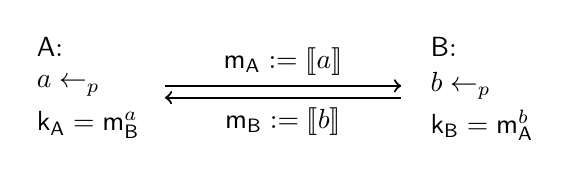
\begin{tikzpicture}
\node [anchor=west] at (2,5) {\A:};
\node [anchor=west] at (7,5) {\B:};
\node [anchor=west] at (2,4.5){$a\leftarrow\Z_p$};
\draw [thick, ->] (3.75,4.5)-- node [midway,above]{$\mes_{\A}:=\lb  a\rb$}(6.75,4.5);
\node [anchor=west] at (7,4.5){$b\leftarrow\Z_p$};
\draw [thick, <-] (3.75,4.35)-- node [midway,below]{$\mes_{\B}:=\lb  b\rb$}(6.75,4.35);
\node [anchor=west] at (2,4) {$\key_\A=\mes_{\B}^a$};
\node [anchor=west] at (7,4) {$\key_\B=\mes_{\A}^b$};
\end{tikzpicture}
\end{minipage}
}
\caption{\label{fig:DH}The figure shows the Diffie-Hellman key exchange. Correctness follows from $\key_\A=\lb  ab\rb=\key_{\B}$.}
\end{figure}
It can be proven secure under the decisional Diffie-Hellman (DDH) assumption.
\begin{definition}[Decisional Diffie-Hellman (DDH) Assumption]
For a group $\G$, the \emph{decisional Diffie-Hellman} assumption is hard if for any ppt distinguisher \D,
$$
|\Pr\lb \D(\lb 1\rb,\lb a\rb,\lb b\rb,\lb ab\rb)=1\rb-\Pr\lb D(\lb 1\rb,\lb a\rb,\lb b\rb,\lb c\rb)=1\rb|=\negl,
$$
where $a\leftarrow\Z_p$, $b\leftarrow\Z_p$ and $c\leftarrow\Z_p$.
\end{definition}

The following lemma states that multi-instance DDH is secure under the DDH assumption with a security loss equal to the amount of instances.

\begin{lemma}\label{lem:DHuniform}
Let DDH be secure over \G except advantage $\epsilon$, then $n$ multi-instance DDH is secure over \G except at most advantage $n\epsilon$.
\end{lemma}

\begin{proof}
This lemma follows from a simple hybrid argument. We define hybrid $\hyb_i$ as the distribution over $\lb \vec{a}\rb,\lb b\rb,\lb \vec{c}\rb$, where for all $j\leq i$, $c_j=a_jb$ and for $j>i$, $c_j\leftarrow\Z_p$. If $\D$ distinguishes hybrid $\hyb_i$ from $\hyb_{i+1}$, it breaks the DDH assumption over \G.
\pe
\end{proof}


\section{Lower Bound on the Round Complexity of Sender and Receiver Chosen Message Security}\label{sec:roundcomp}


In \lemmaref{lem:nosendtweak}, we state that there cannot be an two message OT that achieves sender chosen message security where the sender sends its message first. Here we give the proof. 

\begin{proof}
We show that the most general notion of OT, one out of two OT is impossible.  
For a two message OT where the sender sends its message first, the sender's message $\mes_{\send}$ is a function $f_{\send}$ on input $\tape_{\send}$ and some auxiliary input $\aux$. A sender could sample $s_0,s_1$ during the protocol or receive them as input. We use $\aux$ to cover the second case. Further, there is a function $f_{\rec}$ that takes the random tape $\tape_{\rec}$, $\mes_{\send}$ and choice bit $b$ of $\rec$. Finally, there are two functions $f_{\OT,\send}(\tape_{\send},\mes_{\rec},\aux)$ that outputs $(s_0,s_1)$ and $f_{\OT,\rec}(\tape_{\rec},\mes_{\send},b)$ that outputs $s_b$. 

First, we assume that \send is committed to $(s_0,s_1)$ given $\mes_{\send}$, i.e. there is a $(s_0,s_1)$ such that
$$
\Pr_{\mes_{\rec}, (\tape_{\send},\aux)}[f_{\OT,\send}(\tape_{\send},\mes_{\rec},\aux)=(s_0,s_1)\mid \mes_{\send}=f_{\send}(\tape_{\send},\aux)]\geq\frac{3}{4}.
$$

In this case, a malicious receiver can break the security as follows. It selects two random tapes $\tape_{\rec,1}$, $\tape_{\rec,2}$, two choice bits $b_1=0$, $b_2=1$ and computes for all $i\in[2]$, $\mes_{\rec,i}= f_{\rec}(\tape_{\rec,i},\mes_{\send},b_i)$ and $s_{b_{i},i}=f_{\OT,\rec}(\tape_{\rec,i},\mes_{\send},b_i)$. It outputs $(s_{0,1},s_{1,2})$ as a guess for $s_0,s_1$.

Let the scheme be $\delta$ correct, for $\delta\geq 1-\negl$. Then, the probability that the first malicious receiver reconstructs $(s_0,s_1)$ correctly is lower bounded using Jensen's inequality by
$$
\Pr[(s_{0,1},s_{1,2})=(s_0,s_1)]\geq \left(\frac{3}{4}\delta\right)^2> \frac{1}{2},
$$
where $(s_0,s_1)=f_{\OT,\send}(\tape_{\send},\mes_{\rec},\aux)$. A malicious receiver interacting with the ideal OT can achieve this at most with probability $\frac{1}{2}$. Hence, there is a distinguisher that breaks the sender tweakable security of the OT.

Now assume that for any $(s_0,s_1)$,
\begin{eqnarray}\label{eqn:noncomm}
\Pr_{\mes_{\rec}, \tape_{\send}}[f_{\OT,\send}(\tape_{\send},\mes_{\rec},\aux)=(s_0,s_1)\mid \mes_{\send}=f_{\send}(\tape_{\send},\aux)]<\frac{3}{4}.
\end{eqnarray}
In this case, we show that a malicious receiver can tweak the distribution of $s_0,s_1$.
The malicious receiver uses a hardwired pseudorandom function (PRF) key $\key$ for a PRF $\PRF$ that outputs a single bit.\footnote{OT implies one-way functions and hence also PRFs.} The malicious receiver samples two random tapes $\tape_{\rec,1}$, $\tape_{\rec,2}$, two uniform choice bits $b_1$, $b_2$, computes for all $i\in[2]$ $\mes_{\rec,i}=f_{\rec}(\tape_{\rec,i},\mes_{\send},b_i)$ and $s_{b_i,i}=f_{\OT,\rec}(\tape_{\rec,i},\mes_{\send},b_i)$. If $\PRF_{\key}(s_{b_1,1})=0$ it sends $\mes_{\rec,1}$ to \send and outputs $s_{b_1,1}$ otherwise it sends $\mes_{\rec, 2}$ to \send and outputs $s_{b_2,2}$

 We first give a bound on the probability that $\PRF_{\key}(s_{b_i,i})=0$. Let $\epsilon_{\PRF}$ be a probability such that
$$
\Pr[\PRF_{\key}(s_{b_i,i})=0]= \frac{1}{2}-\epsilon_{\PRF}.
$$
Then there is a distinguisher $\D$ that simply outputs $1$ if $\PRF_{\key}(s_{b_i,i})=0$. Hence,
$$
|\Pr[\D(1^\sec,s_{b_i,i},\PRF_{\key}(s_{b_i,i}))=1]-\Pr[\D(1^\sec,s_{b_i,i},u)=1]|=\epsilon_{\PRF},
$$  
where $u\leftarrow\bits$. Since $\D$ breaks \PRF with probability $\epsilon_{\PRF}$ and \PRF is secure, $\epsilon_{\PRF}$ is negligible. By $(\ref{eqn:noncomm})$, it holds with at least probability $\frac{3}{16}$ that $s_{b_1,1}\neq s_{b_2,2}$. Therefore, the probability that for the output $s_{b_i,i}$ of the malicious holds $\PRF_{\key}(s_{b_i,i})=0$ is at least
\begin{eqnarray*}
\lefteqn{\Pr[\PRF_{\key}(s_{b_i,i})=0]}\\
&=&\Pr[\PRF_{\key}(s_{b_1,1})=0]+\Pr[\PRF_{\key}(s_{b_1,1})=1\wedge\PRF_{\key}(s_{b_2,2})=0]\\
&\geq&  \left(\frac{1}{2}-\epsilon_{\PRF}\right)+\left(\frac{1}{2}+\epsilon_{\PRF}\right)\cdot\frac{3}{16}\left(\frac{1}{2}-\epsilon_{\PRF}\right)\\
&=& \frac{1}{2}+\frac{1}{64}-\negl.
\end{eqnarray*}
Since the OT is $\delta=1-\negl$ correct, we get by using a union bound that the malicious receivers output $s_{b_i,i}$ is correct and $\PRF_{\key}(s_{b_i,i})=0$ holds at least with probability $\frac{1}{2}+\frac{1}{64}-\negl$. Hence, $\PRF_{\key}(s_{b_i,i})=0$ holds with a noticeable bias - given $\key$- when the malicious receiver interacts with an honest sender. If there is a distribution of $(s_0,s_1)$ from which the ideal OT samples with the same bias, then there is a distinguisher $\D$ that breaks the security of \PRF. $\D$ samples from this distribution, queries $\PRF$ on the samples and outputs $1$ if the query returns $0$. 

Since there is no such a distribution for a secure PRF, there is no adversary $\Adv'$ that creates the same output distribution when interacting with the ideal OT as when the malicious receiver interacts with the honest sender. Hence, the OT is not sender chosen message secure. 
\pe
\end{proof}

The following proof is the proof for \lemmaref{lem:norectweak}, which states that there cannot be an two message OT that achieves receiver chosen message security where the receiver sends its message first.

\begin{proof}
Again, we rule out the most general notion of OT, one out of two OT. We follow a similar strategy as in the previous lemma.
A two message OT where the receiver sends its message first has the following structure. The receiver's message $\mes_{\rec}$ is a function $f_{\rec}$ on input $\tape_{\rec}$, $b$ and some auxiliary input $\aux$. Further, there is a function $f_{\send}$ that takes the random tape $\tape_{\send}$ and $\mes_{\rec}$ as input. Finally, there are two functions $f_{\OT,\send}(\tape_{\send},\mes_{\rec})$ that outputs $(s_0,s_1)$ and $f_{\OT,\rec}(\tape_{\rec},\mes_{\send},b,\aux)$ that outputs $s_b$. 

We distinguish two cases. In case one,  we assume that \rec is committed to $s_b$ given $\mes_{\rec}$, i.e. there is a $s_b$ such that
$$
\Pr_{\mes_{\send}, (\tape_{\rec},b,\aux)}[f_{\OT,\rec}(\tape_{\rec},\mes_{\send},b,\aux)=s_b\mid \mes_{\rec}=f_{\rec}(\tape_{\rec},b,\aux)]=\frac{3}{4}+\alpha,
$$
for $\alpha\geq 0$.
Further, $s_{\overline b}$ should not be determined by $\mes_{\rec}$. Let $\ell$ be the length of $s_0$, $s_1$, then if there is a $s_{\overline b}$ s.t. 
$$
\Pr_{\tape_{\send}}[s_{\overline b}\text{ is output of }f_{\OT,\send}(\tape_{\send},\mes_{\rec})\text{ for bit }\overline b\mid \mes_{\rec}]=\frac{1}{2^\ell}+\epsilon,
$$
then a malicious receiver can sample $\tape_{\send}$ and compute $f_{\OT,\send}(\tape_{\send},\mes_{\rec})$ to learn $s_{\overline b}$ with probability $\frac{1}{2^\ell}+\epsilon-(1-\delta)$, where OT is $\delta=1-\negl$ correct. Since the ideal primitive samples $s_{\overline b}$ at uniform, the malicious receiver breaks the OT with probability $\epsilon-\negl$. Therefore, $\epsilon=\negl$. 

But now, a malicious sender can sample two random tapes $\tape_{\send,1}$, $\tape_{\send,2}$
and compute for all $i\in[2]$, $(s_{0,i},s_{1,i})=f_{\OT,\send}(\tape_{\send,i},\mes_{\rec})$ and checks for all $i\in\bits$ whether $s_{i,1}=s_{i,2}$. It outputs a random $b'$ if it holds for both or no $i\in\bits$, otherwise it outputs $b'$ such that $s_{b',1}=s_{b',2}$. It holds that
$$
\Pr[s_{b,1}=s_{b,2}]= \left(\frac{3}{4}+\alpha\right)^2+\left(\frac{1}{4}-\alpha\right)^2\frac{1}{2^\ell-1}\\
\geq \frac{9}{16}
$$
%\frac{9}{16}+\frac{1}{16(n-1)}+\frac{3(n-1)+1}{2(n-1)}\alpha+\frac{n}{n-1}\alpha^2
and
$$
\Pr[s_{\overline{b},1}=s_{\overline{b},2}]\geq \frac{1}{2^\ell}-\epsilon.
$$
Therefore,
\begin{eqnarray*}
\lefteqn{\Pr[b=b']}\\
&=&\frac{1}{2}\Pr[\nexists! i:s_{i,1}= s_{i,2}]+\Pr[s_{b,1}=s_{b,2}\wedge s_{\overline b,1}\neq s_{\overline b,2}]-(1-\delta)\\
&\geq& \frac{2^\ell-1}{2^{\ell+1}}-\frac{2^\ell-2}{2^{\ell+1}}\Pr[s_{b,1}=s_{b,2}]+\frac{2^\ell-1}{2^\ell}\Pr[s_{b,1}=s_{b,2}]
-\negl\\
&\geq & \frac{2^{\ell}-1}{2^{\ell+1}}+\frac{2^{\ell}}{2^{\ell+1}}\frac{9}{16}-\negl\geq
\frac{1}{2}+\frac{1}{32}-\frac{1}{2^{\ell+1}}+\frac{1}{4}-\negl
\end{eqnarray*}
where we apply a union bound to argue that the outputs are correct and corresponds to the receivers choice. Given that $\ell\geq 1$, the malicious sender guesses $b$ correctly with at least probability $\frac{1}{2}+\frac{1}{32}-\negl$. Since in the ideal model, an adversary can guess $b$ only with probability $\frac{1}{2}$, this constitutes a break of receiver tweakable security.

In the case two, for any $s_b$,
$$
\Pr_{\mes_{\send}, (\tape_{\rec},b,\aux)}[f_{\OT,\rec}(\tape_{\rec},\mes_{\send},b,\aux)=s_b\mid \mes_{\rec}=f_{\rec}(\tape_{\rec},b,\aux)]<\frac{3}{4}.
$$
Similar as in the proof of Lemma~\ref{lem:nosendtweak}, we argue that a malicious sender can tweak the output distribution of $(s_0,s_1)$. Due to the similarity, we only exhibit a brief version. Again we hardwire a PRF key $\key$ for a PRF with a single output bit. Given $\mes_{\rec}$, the malicious sender samples two random tapes $\tape_{\send, 1}$ and $\tape_{\send,2}$, computes for all $i\in[2]$ $(s_{0,i},s_{0,i})=f_{\OT,\send}(\tape_{\send,i},\mes_{\rec})$. If $\PRF_{\key}(s_{0,1},s_{1,1})=0$ output $(s_{0,1},s_{1,1})$ and send $\mes_{\send,1}=f_{\send}(\tape_{\send,1},\mes_{\rec})$ to \rec. Otherwise output $(s_{0,2},s_{1,2})$ and send $\mes_{\send,2}=f_{\send}(\tape_{\send,2},\mes_{\rec})$ to \rec. This way, $\Pr_{\key}(s_0,s_1)=0$ holds for the malicious sender's output $(s_0,s_1)$ with probability 
\begin{eqnarray*}
\lefteqn{\Pr[\PRF_{\key}(s_0,s_1)=0]}\\
&=&\Pr[\PRF_{\key}(s_{0,1},s_{1,1})=0]+\Pr[\PRF_{\key}(s_{0,1},s_{1,1})=1\wedge\PRF_{\key}(s_{0,2},s_{1,2})=0]\\
&\geq&  \left(\frac{1}{2}-\epsilon_{\PRF}\right)+\left(\frac{1}{2}+\epsilon_{\PRF}\right)\cdot\frac{3}{8}\left(\frac{1}{2}-\epsilon_{\PRF}\right)\\
&=& \frac{1}{2}+\frac{1}{32}-\negl,
\end{eqnarray*}
unless one breaks the security of the PRF. As previously, this constitutes an attack against the receiver chosen message security.
\pe
\end{proof}



\section{All But One OT from Key Agreement}\label{sec:allbutone}

In this section we show how to use the techniques in \namedref{Section}{sec:endemicOT} to construct an all but one, i.e. $n-1$ out of $n$, OT. We show the protocol in \figureref{fig:allbutone} and give a state the achieved security in \namedref{Lemma}{lem:allbutone} without giving a detailed proof. Security follows from the same reasoning as in \namedref{Section}{sec:endemicOT}.

\begin{figure}
\centering
\framebox{
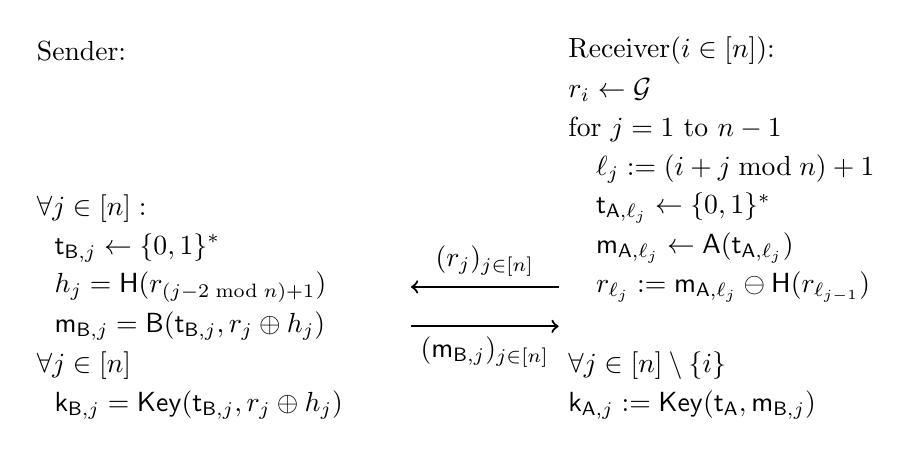
\begin{tikzpicture}[xscale=1.5]
\node [anchor=west] at (-0.5,5) {Sender:};
\node [anchor=west] at (4,5) {Receiver$(\i\in[n])$:};
\node [anchor=west] at (4,4.5){$r_{i}\leftarrow\G$};
\draw [thick, <-] (2.75,2)-- node [midway,above]{$(r_j)_{j\in[n]}$}(4,2);
\node [anchor=west] at (-0.5,3){$\forall j\in[n]:$};
\node [anchor=west] at (-0.35,2){$h_j=\H(r_{(j-2\bmod n)+1})$};
%\node [anchor=west] at (-0.35,2.5){$\mes_{\A,j}=r_j\oplus h_j$};
\node [anchor=west] at (-0.35,2.5){$\tape_{\B,j}\leftarrow\bits^*$};
\node [anchor=west] at (-0.35,1.5){$\mes_{\B,j}=\B(\tape_{\B,j},r_j\oplus h_j)$};
\draw [thick, ->] (2.75,1.5)-- node [midway,below]{$(\mes_{\B,j})_{j\in[n]}$}(4,1.5);
\node [anchor=west] at (-0.5,1) {$\forall j\in[n]$};
\node [anchor=west] at (-0.35,0.5) {$\key_{\B,j}=\EK(\tape_{\B,j},r_j\oplus h_j)$};
\node [anchor=west] at (4,4){for $j=1$ to $n-1$};
\node [anchor=west] at (4,3.5){$\quad\ell_{j}:=(i+j\bmod n) +1$};
\node [anchor=west] at (4,3){$\quad\tape_{\A,\ell_j}\leftarrow\bits^*$};
\node [anchor=west] at (4,2.5){$\quad\mes_{\A,\ell_j}\leftarrow \A(\tape_{\A,\ell_j})$};
\node [anchor=west] at (4,2){$\quad r_{\ell_j}:=\mes_{\A,\ell_j}\ominus\H(r_{\ell_{j-1}})$};
\node [anchor=west] at (4,1) {$\forall j\in[n]\setminus\{\i\}$}; 
\node [anchor=west] at (4,0.5) {$\key_{\A,j}:=\EK(\tape_\A,\mes_{\B,j})$};
\end{tikzpicture} 
}
\myvspace{-0.3cm}
\caption{The figure shows a $n-1$ out of $n$ OT using a $\UKA=(\A,\B,\EK)$ and a random oracle $\H:\G\rightarrow\G$, where \G is a group with operations $\oplus$, $\ominus$. By the correctness of the \UKA scheme, $\key_{\A,\i}=\key_{\B,\i}$ holds. The scheme can be transformed in the same way in a one-round scheme given a one-round \UKA as in the $1$ out of $n$ OT case in \namedref{Section}{sec:endemicOT}.}
\label{fig:allbutone}
\end{figure}
 
\begin{lemma}\label{lem:allbutone}
Given a correct and secure \UKA scheme, then the $n-1$ out of $n$ oblivious transfer in  \figureref{fig:allbutone} is an Endemic $\OT_{n-1,n}$ in the programmable random oracle model. 
\end{lemma}

\begin{proof}
The proof is very similar to the security proof of the $1$ out of $n$ OT. In fact, the proof is even simpler since the random oracle receives only a single $r$ as input and for a malicious receiver, distinguishing a single string, i.e. $\key_{i}$, needs to be hard. This even removes some of the complexity of the previous proof. In the following, we state the claims, which only require minor adaptations to the claims of the previous proofs. For this reason, we do not give their proofs here. 

Security against a malicious sender follows by the claim below. 
\begin{claim}\label{claim:malsender}
Given a $\delta$ correct and $\epsilon$ uniform \UKA scheme, then it holds that in the programmable random oracle model for any ppt adversary \Adv, there exists a ppt adversary \Adv' such that for any ppt distinguisher \D and any polynomial size auxiliary input $z$
$$
|\Pr[\D(z,(\Adv,\rec)_{\Pi})=1] -\Pr[\D(z, (\Adv', \OOT^\send))=1]|\leq \epsilon+(1-\delta),
$$
where all algorithms receive input $1^\sec$ and \rec additionally receives input \set.
\end{claim}


By a second claim, the protocol is secure against a malicious receiver.
\begin{claim}\label{claim:malreceiver}
Given a $\delta$ correct,  $Q$-multi-instance $\epsilon_u$-uniform,  $(Q,1)$-multi-instance $\epsilon_k$-key-indistinguishable  \UKA scheme, where $Q$ upper bounds the amount of random oracle queries by an adversary then it holds that in the programmable random oracle model for any ppt adversary \Adv, there exists a ppt adversary \Adv' such that for any ppt distinguisher \D and any polynomial size auxiliary input $z$
$$
|\Pr[\D(z,(\send, \Adv)_{\Pi})=1] -\Pr[\D(z,(\OOT^\rec,\Adv'))=1]|\leq Q(\epsilon_{u}+\epsilon_{k})+(1-\delta),
$$
where all algorithms receive input $1^\sec$.
\end{claim}
\pe
\end{proof}


\section{Instantiations}\label{sec:inst}
In the following, we first show how to efficiently instantiate the construction in \figureref{fig:oneroundKAtoOT} using the Diffie-Hellman key exchange. In particular, we show how a tighter security reduction can be obtained using the random selfreducibility of the DDH assumption.

Afterwards, we show how to instantiate the construction in \figureref{fig:KAtoOT} based on the lattice based Kyber key agreement. 
\newcommand{\Z}{\ensuremath{\mathbb Z}\xspace}

\subsection{Instantiation from DDH}

In this subsection we use a group \G of prime order $p$ and $g$ is a generator or \G. For simplicity, we use the bracket notation $\lb a\rb$ to denote $g^a$, in particular $\lb 1\rb:=g$. For vector $\vec{a}=(a_1,\ldots,a_n)$, we use $\lb \vec{a}\rb$ to denote $(\lb a_1\rb,\ldots,\lb a_n\rb)$. We use the same notation, i.e. $\lb A\rb$, also for a matrix $A$.



\begin{definition}[$n$ Multi-Instance DDH Assumption]
For a group $\G$, the \emph{decisional Diffie-Hellman} assumption is hard if for any ppt distinguisher \D,
$$
|\Pr\lb \D(1^\sec,\lb 1\rb,\lb \vec{a}\rb,\lb b\rb,\lb \vec{a}b\rb)=1\rb-\Pr\lb D(1^\sec,\lb 1\rb,\lb \vec{a}\rb,\lb b\rb,\lb \vec{c}\rb)=1\rb|=\negl,
$$
where $\vec{a}\leftarrow\Z_p^n$, $b\leftarrow\Z_p$ and $\vec{c}\leftarrow\Z_p^n$.
\end{definition}

In Appendix~\ref{sec:DDH}, we show that $n$ multi-instance DDH is secure under the DDH assumption with a security loss of $n$. In the following we show that the Diffie-Hellman key exchange is tightly multi-instance secure under multi-instance DDH. 

\begin{lemma}\label{lem:DDH}
Let $Q$ and $n$ be polynomial in $\sec$.
The Diffie-Hellman key exchange over \G is unconditionally $Q$ multi-instance uniform. Further, let the $n$ multi-instance DDH assumption hold over group \G except with advantage $\epsilon$, then the Diffie-Hellman key exchange is $(Q,n)$ one-round multi-instance key indistinguishable except advantage $\epsilon-\negl$. 
\end{lemma}

\begin{proof}
The distribution of $\lb a\rb$ over \G is uniform, therefore 
$$
|\Pr\lb \D^{\O_{\A}}(1^{\sec})\rb=1\rb-Pr\lb \D^{\O_{u}}(1^{\sec})=1\rb|=0,
$$
even against an unbounded $\D$. Hence, the Diffie-Hellman key exchange is unconditional $Q$ multi-instance uniform.

For proving the second part of the lemma, we construct a ppt distinguisher \D that breaks $n$ multi-instance DDH assumption given a ppt distinguisher $\D_\key$ that breaks the $(Q,n)$ multi-instance key indistinguishability of the Diffie-Hellman key exchange. $\D$ receives a challenge $\lb \vec{a}\rb,\lb b\rb,\lb \vec{c}\rb$, sets $\mes_{\B}:=\lb b\rb$ and invokes $\D_{\key}$ on input $\mes_{\B}$. On the $j$-th query of $\D_{\key}$ to $\O_{\A}$, \D samples $\vec{r}_j\leftarrow\Z_p^{n+1}$ and responds with $\mes_{\A,j}:=\lb \langle (\vec{a},1),\vec{r}_j\rangle\rb=\lb a_1\rb^{r_{j,1}}\cdot\lb a_2\rb^{r_{j,2}}\ldots\lb a_n\rb^{r_{j,n}}\cdot\lb r_{j,n+1}\rb$. When $\D_{\key}$ queries $\O_{\key}$ for key $\key_j$, \D responds with $\key_j:=\lb \langle\vec{c},\vec{r}_j\rangle\rb=\lb c_1\rb^{r_{j,1}}\cdot\lb c_2\rb^{r_{j,2}}\ldots\lb c_n\rb^{r_{j,n}}\cdot\lb b\rb^{r_{j,n+1}}$. In the end, $\D$ outputs the output of $\D_{\key}$.

It is easy to see that $\O_{\A}$ has the correct output distribution. $r_{j,n+1}$ is uniform over $\Z_p$ and hence $\mes_{\A,j}$ is. Further, conditioned on $\mes_{\A,j}$, $r_{j,1},\ldots,r_{j,n}$ are uniform. Given that $\vec{c}=\vec{a}b$, the output
$$
\key_j=\lb \langle\vec{c},\vec{r}_j\rangle\rb\cdot\lb b\rb^{r_{j,n+1}}=\lb \langle\vec{a}b,\vec{r}_j\rangle\rb\cdot\lb b\rb^{r_{j,n+1}}=\lb \langle(\vec{a},1),\vec{r}_j\rangle\rb^b=\mes_{\A,j}^b
$$
of $\O_{\key}$ is also distributed correctly. In case that $\vec{c}$ is uniform, we need to show that all the $n$ outputs of $\O_{\key}$, $\vec{\key}=\key_1,\ldots,\key_n$ are uniform. Let $\mes_i$ be the message $\mes_{\A,j}$ and $\vec{t}_i$ the randomness $\vec{r}_j$ that corresponds to $\key_i$. Since $\vec{c}$ is uniform and $\vec{\key}=\lb \vec{c}\cdot T\rb$, where $T$ is the matrix with $i$-th column $\vec{t}_i$, $\vec{\key}$ is uniform if $T$ is invertible. Since $r_{j,1},\ldots,r_{j,n}$ are uniform given $\mes_{\A,j}$ so is $T$. For a uniform $T$ over $\Z_p^{n\times n}$, the probability that $T$ is invertible is that all the rows are linear independent, i.e. 
$$
\Pr\lb T\text{ invertible}\rb= \frac{1}{p^{n^2}}\prod_{i=0}^{n-1}(p^n-p^i)\geq\left(1-\frac{1}{p}\right)^n\geq 1-\negl.
$$ 
Therefore, except with negligible probability, $\D$ has the same advantage in breaking $n$ multi-instance DDH as $\D_{\key}$ has in breaking $(Q,n)$ one-round multi-instance key indistinguishability.
\pe
\end{proof}

Using Theorem~\ref{thm:KAtoOT}, Lemma~\ref{lem:DHuniform} and Lemma~\ref{lem:DDH}, we obtain the following corollary.

\begin{corollary}
When instantiating an $1$ out of $n$ OT in \figureref{fig:oneroundKAtoOT} with Diffie-Hellman key exchange over group \G, then in the programmable random oracle model the resulting endemic OT is statistically secure against malicious senders making at most polynomially many random oracle queries and secure against malicious receivers except advantage $(n-1)Q\epsilon_{\DDH}+\negl$, where the DDH assumption over group $\G$ holds except advantage $\epsilon_{\DDH}$ and $Q$ is a bound on the amount of adversarial random oracle queries.
\end{corollary}

\begin{remark}
If we apply a hardcore predicate to $\key_{\A}$ and $\key_{\B}$ in the protocol in \figureref{fig:DH} and apply the transformation \figureref{fig:oneroundKAtoOT}, we receive a one-round endemically secure OT in the random oracle model based on the computational Diffie-Hellman assumption. Alternatively, one could also use the random oracle instead of a hardcore predicate to obtain longer OT strings. 
\end{remark}

\subsection{Instantiation based on Crystals-Kyber}
 

\begin{figure}[h!]
\centering
\framebox{
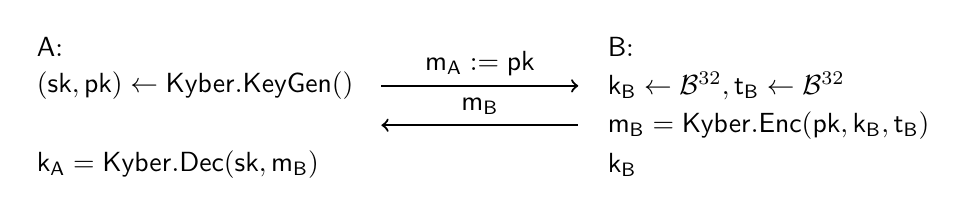
\begin{tikzpicture}
\node [anchor=west] at (-0.25,5) {\A:};
\node [anchor=west] at (7,5) {\B:};
\node [anchor=west] at (-0.25,4.5){$(\sk,\pk)\leftarrow\kybergen()$};
\draw [thick, ->] (4.25,4.5)-- node [midway,above]{$\mes_\A:=\pk$}(6.75,4.5);
\node [anchor=west] at (7,4.5){$\key_{\B}\leftarrow\kB^{32},\tape_\B\leftarrow\kB^{32}$};
\node [anchor=west] at (7,4){$\mes_\B=\kyberenc(\pk, \key_{\B},\tape_\B)$};
\draw [thick, <-] (4.25,4)-- node [midway,above]{$\mes_\B$}(6.75,4);
\node [anchor=west] at (-0.25,3.5) {$\key_\A=\kyberdec(\sk,\mes_\B)$};
\node [anchor=west] at (7,3.5) {$\key_\B$};
\end{tikzpicture}
}
\label{fig:Kyber}
\caption{The figure shows a Kyber based key agreement protocol between parties \A and \B.}
\end{figure}

\begin{definition}[Crystals-Kyber CPAPKE]
\emph{ Crystals-Kyber CPAPKE} is a correct and CPA secure public key encryption based on the Module LWE (\MLWE) assumption. We follow the specifications of Kyber, in which $\kB$ denotes the  set $\{0,1,\ldots,255\}$. Kyber is parameterized by parameters $d_t=11$, $\nLWE=256$, $\kLWE\in\{2,3,4\}$, $q=7681$ and ring $\R_q=\Z_q\lb X\rb/(X^{\nLWE}+1)$. 

$(\kybergen,\kyberenc,\kyberdec)$ have the following syntax. 
\begin{description}
\item[$\kybergen$:] Outputs a secret and public key pair $\pk,\sk$, where $\pk=(\cdt,\rho)\in\kB^{\frac{\kLWE\nLWE d_t}{8}}\times\kB^{32}$.
\item[$\kyberenc$:] Takes as input a public key $\pk$, a message $\mes\in\kB^{32}$ and random coins $\tape\in\kB^{32}$. It outputs a ciphertext $\kyberc$.
\item[$\kyberdec$:] Takes as input secret key $\sk$ and a ciphertext $\kyberc$. It outputs a message $\mes$.
\end{description}
Further, Crystals-Kyber specifies the following algorithms.
\begin{description}
\item[$\kdec_\ell$:] Takes a an element in $\kB^{32\ell}$ and maps it to $\R_q$. The inverse operation is $\kenc_\ell$.
\item[$\kcom_q(*,d)$:] Takes a an element in $\R_q$ and maps it to a polynomial with coefficients in $\Z_{2^d}$. The inverse operation is $\kdecom_q(*,d)$.
\item[$\kparse$:] Takes a uniform byte stream in $\kB^{*}$ and maps it to a uniform element in $\R_q$.
\end{description}
\end{definition}

It is important to know, that $\cdt:=\kenc_{d_t}(\kcom_q(\mt, d_t)$, where $\mt$ is computationally indistinguishable from a uniform element in $\R_q^{\kLWE}$ based on the \MLWE assumption. In the following, we will choose $d_t=13$ such that $q<2^{d_t}$ and no compression takes place. This will help us to avoid complications and does not decrease efficiency besides a sligthly larger public key $\pk$. Further, we will keep component $\rho$ of $\pk$ consistent between all $\pk$ used in a single $1$ out of $n$ OT.

In order to instantiate our framework, we need to define a group operation $\pk\oplus\pk$ and a hash functions that maps to a uniform $\cdt$ component of $\pk$, i.e. a uniform element in $\R_q^{\kLWE}$. For the latter, we use a hash function that produces an output bit stream, which is in $\kB^{*}$, and use $\kLWE$ different parts of the stream and apply $\kparse$ to the $\kLWE$ streams to obtain a (pseudo) uniform element in $\R_q^{\kLWE}$ whenever the bit streams are (pseudo) uniform.

We define the group operation $\pk_1\oplus\pk_2$, by mapping $\pk_1=(\cdt_1,\rho)$, $\pk_2=(\cdt_2,\rho)$ to $\pk_3=(\cdt_3, \rho)$, where $\cdt_3=\kenc_{13}(\kdec_{13}(\cdt_1)+\kdec_{13}(\cdt_2))$ and $+$ is the addition in $\R_q^{\kLWE}$. $\ominus$ is defined correspondingly. 

By using \theoremref{thm:KAtoOT}, \lemmaref{lem:multuniform} and \lemmaref{lem:keytomultkey}, we get the following corollary.
 
\begin{corollary}
When instantiating an $1$ out of $n$ OT in \figureref{fig:oneroundKAtoOT} with Crystals-Kyber, then in the programmable random oracle model the resulting endemic OT is secure against a malicious sender except advantage $(n-1)\epsilon_{\MLWE}+\negl$  and secure against malicious receivers except advantage $Q^2\epsilon_{\MLWE}+\negl$, where the \MLWE assumption holds except advantage $\epsilon_{\MLWE}$ and $Q$ is a bound on the amount of adversarial random oracle queries.
\end{corollary}

In the following, we will instatiate Kyber with $k=3$ which is claimed to have a qbit security level of $161$ bit. This security level does not immediatly carry over to our Kyber based OT, there is an additional security loss of $Q^2$. Though we are unaware of an attack that is significantly more efficient on our Kyber based OT than the attacks on Kyber.
%
\iffullversion
\else
\section{Instantiation Appendix}

\begin{figure}[h!]
\centering
\framebox{
\begin{minipage}{0.85\linewidth}
\centering
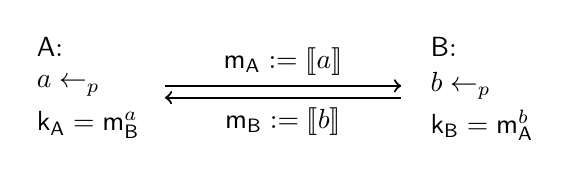
\begin{tikzpicture}
\node [anchor=west] at (2,5) {\A:};
\node [anchor=west] at (7,5) {\B:};
\node [anchor=west] at (2,4.5){$a\leftarrow\Z_p$};
\draw [thick, ->] (3.75,4.5)-- node [midway,above]{$\mes_{\A}:=\lb  a\rb$}(6.75,4.5);
\node [anchor=west] at (7,4.5){$b\leftarrow\Z_p$};
\draw [thick, <-] (3.75,4.35)-- node [midway,below]{$\mes_{\B}:=\lb  b\rb$}(6.75,4.35);
\node [anchor=west] at (2,4) {$\key_\A=\mes_{\B}^a$};
\node [anchor=west] at (7,4) {$\key_\B=\mes_{\A}^b$};
\end{tikzpicture}
\end{minipage}
}
\caption{\label{fig:DH}The figure shows the Diffie-Hellman key exchange. Correctness follows from $\key_\A=\lb  ab\rb=\key_{\B}$.}
\end{figure}
\fi

\section{OT Extension Appendix}\label{sec:extApp}


\iffullversion
\else

\subsection{Definition of \definitionref{def:ext_S_R}}

\begin{definition}\label{def:ext_S_R}
	Let $\Pi^{\textsf{ext-S}u\pi}$ be the protocol of \figureref{fig:otExt} where $\OOT:=\OOT^{\send u}$ and the random oracle $\H(i,x)$ required by $\Pi^{\textsf{ext-E}}$ is replaced as follows: $\H(x)=\pi(x)+x$ where $\pi:\{0,1\}^{\kappa} \times \mathbb{F}^\nc_2 \rightarrow\{0,1\}^\kappa$ is an ideal permutation. Note: the $i$ parameter of $\H$ is removed.
\end{definition}
\begin{lemma}\label{lem:ext_S_R}
	The $\Pi^{\textsf{ext-S}u\pi}$ protocol realizes 1-out-of-$N$ $\OOT^\rec$-security, for $N=\textsf{poly}(\kappa)$.
\end{lemma}
\begin{proof}
	See full version.
\end{proof}


\subsection{Proof of \lemmaref{lem:malRec}}



\begin{proof}\label{proof:Attack_BadT0}
	For simplicity let $N=2$ and $m=1$. We define $\Adv$ as follows. $\Adv$ plays the role of \rec and replaces the input to base OTs, the sender input, with strings $\tt_0^j,\tt_1^j\in \{0\}^{m'}$ and then completes the protocol as normal.
	
	We define $D$ as follows. $D$ executes \send and \Adv with input $x_1=1$. \send outputs $(\vv_{1,1},\vv_{1,2})$ and $D$ outputs 1 if $\vv_{1,1}=\H(1, \{0\}^\nc)$ and 0 otherwise. In the real interaction it clearly holds that $\Pr[D((\send, \Adv)_{\langle\send, \Adv\rangle})=1]=1$. In the ideal interaction the honest \send will output a uniformly distributed $\vv_{1,1}\in\{0,1\}^\kappa$ which was sampled by $\OOT^{\U}$ and therefore $\Pr[D((\O^{\U}_{\textsf{OT,\send}}, \Adv')_{\langle\OOT^\U, \Adv'\rangle})=1]=2^{-\kappa}$.
\end{proof}


\subsection{Proof of \lemmaref{lem:malRec2}}

\begin{proof}\label{proof:Attack_Selection}
	For simplicity let $N=2$ and $m=\kappa$. We define $\Adv$ as follows. $\Adv$ plays the role of \rec and receives the strings $\tt_0^j,\tt_1^j\in \{0\}^{m'}$ from \OOT. $\Adv$ redefines the selection values $x_1,...,x_m\in[2]$ of \rec such that $x_i:=\textsc{lsb}(\H(i, \tt_i))+1$. That is, $x_i$ equals the least significant bit of $\vv_{i,x_i}=\H(i, \tt_i)$ plus 1. \Adv executes the rest of the protocol as \rec would and outputs $(x_i)_{i\in [m]}$.
	
	We define $\D$ as follows. $\D$ executes \send and \Adv. \send outputs $(\vv_{i,1},\vv_{i,2})_{i\in[m]}$ and $\D$ outputs 1 if $\forall i\in[m], \textsc{lsb}(\vv_{i,x_i})+1=x_i$ and 0 otherwise. In the real interaction it clearly holds that $\Pr[\D((\send, \Adv)_{\Pi^{\textsf{OOS+}}})=1]=1$. In the ideal interaction the honest \send will output a uniformly distributed $\vv_{i,1},\vv_{i,2}\in\{0,1\}^\kappa$ which are independent of $x_i$ and therefore $\Pr[\D((\OOT^{\U}, \Adv'))=1]=2^{-\kappa}$.
	\pe
\end{proof}



\subsection{Proof of \lemmaref{lem:malSend}}
\begin{proof} \label{proof:Attack_AllOnes}
	For simplicity let $N=2$ and $m=\kappa$. We define $\Adv$ as follows. $\Adv$ plays the role of \send and replaces the input to $\OOT^\send$, the receiver input, with the string $\bb:=\{0\}^\nc$. \Adv outputs the matrix $Q$.
	
	We define $D$ as follows. $D$ samples the selection bits $x_1,...,x_m\gets[2]$ and sends them to \rec. $D$ executes $\Adv$ who outputs $Q$ and \rec outputs $\vv_{1,x_1},...,\vv_{m,x_m}$. If $\vv_{i,x_i}=\H(i,\qq_i)$ for all $i\in[m]$, output 1, otherwise 0. In the real interaction it clearly holds that $\Pr[D((\Adv, \rec)_{\langle\Adv,\rec\rangle})=1]=1$ since $\qq_i=\tt_i$.
	
	By definition the input of $\Adv'$ is independent of $x_i$ and receives no output from $\OOT^\E$ (apart from their input $(\vv_{0,i},\vv_{1,i})_{i\in [m]}$). Therefore, it must hold that $\Pr[D((\Adv', \rec)_{\langle\Adv',\O^{\E}_{\textsf{OT,\send}}\rangle})=1]=2^{\kappa}$.
\end{proof}


\subsection{Proof of \lemmaref{lem:ext_R_S}}

\begin{proof}\label{proof:ext_R_S}
		\begin{claim}[Malicious Sender Security]\label{claim:ext-R-S-MalSender}
		$\Pi^{\textsf{ext-R}}$ satisfies Security Against a Malicious Sender (\definitionref{def:otSec}) with respect to the $\OOT^\send$ oracle.
	\end{claim}
	\begin{proof}
		%The simulation follows the same strategy as \lemmaref{lem:ext-E} except now $\Adv$ is allowed to sample $k$ and influence the messages being output by the parties. In particular, after \Adv sends $k$ to $\Adv'$, $\Adv'$ defines the circuits $\mathcal{M}_i(x)=\pi_k(y)+y$ where $y:=\tt_i + \bb \odot (\cc_i + \mathcal{C}(map(x)))$ and sends it to $\OOT^\send$ and the input of \send.
		
		The simulation follows essentially the same strategy as \lemmaref{lem:ext-E}. Consider the following hybrids which will define the simulator $\Adv'$. 
		\begin{enumerate}[leftmargin=1.8cm]
			\item[Hybrid 1.] $\Adv'$ internally runs \Adv while plays the role of $\rec$ and base OT oracle $\OOT=\OOT^\rec$. For $j\in[\nc]$, $\Adv'$ receives $(\bb'_j,\tt^j_{\bb_j})\in [2]\times \mathbb{F}^{m'}_2$ from \Adv in \stepref{step:extInit} where $\bb_j:=\bb_j'-1$. $\Adv'$ uniformly samples $\tt^j_{1-\bb_j}$ as $\OOT=\OOT^\E$ would. $\Adv'$ sends $(\bb', \{\tt^j_{\bb}\})$ to $\Adv$ on behalf of \OOT. $\Adv'$ outputs whatever \Adv outputs. The view of $\Adv$ is unmodified.
			
			\item[Hybrid 2.] For \stepref{step:extSendU} $\Adv'$ does not sample $\tt^j_{1-\bb_j}$ and instead uniformly samples $U\gets\mathbb{F}^{m'\times \nc}_2$. $\Adv'$ sends $U$ to \Adv and then computes $Q$ as \send would. The view of $\Adv$ is identically distributed. This follows from the fact that $\tt^j_{1-\bb_j}$ is uniformly distributed in the view of \Adv and masks the $j$-th column of $U$ in the previous hybrid. 
			
			\item[Hybrid 3.] For \stepref{step:consistency} $\Adv'$ simulates the consistency proof. This change is indistinguishable. 
			
			\item[Hybrid 4.]\label{hybrid:mmmm} $\Adv'$ receives $k$ from $\Adv$ as specified in \definitionref{def:ext_R_S}. For each row $\qq_i$, $\Adv'$ defines the circuit $\mathcal{M}_i:[N]\rightarrow\{0,1\}^\kappa$ such that on input $j\in[N]$ it outputs $\H( \qq_i+\bb\odot \mathcal{C}(map(j)))$. $\Adv'$ sends $\mathcal{M}_i$ to the ideal oracle $\OOT^\E$ as the sender's input to the $i$-th OT instance. This change allows the ideal oracle to output the same distribution as the real protocol. The view of $\Adv$ is unmodified.
			
			Let $y_{j}= \qq_i+\bb\odot \mathcal{C}(map(j))=\tt_i + \bb \odot (c_i + \mathcal{C}(map(j))$ and note that $\Adv$ can influence $\mathcal{M}_i(j)=\H(y_j)=\pi_k(y_j)+y_j$ by choosing $k,\bb$ and the bits $\{\tt_i[j] \mid \bb_j=0\}$.
			
			\item[Hybrid 5.] $\Adv'$ does not take the input of \rec. \rec only interacts with $\OOT^\E$. This change is identically distributed since $\Adv'$ was not using the input of \rec.
		\end{enumerate}
	\end{proof}
	\begin{claim}[Malicious Receiver $\OOT^\U$-Security]\label{claim:ext-R-S-MalReceiver}
		$\Pi^{\textsf{ext-R}}$ satisfies Security Against a Malicious Receiver (\definitionref{def:otSec}) with respect to the $\OOT^\U$ oracle.
	\end{claim}
	\begin{proof}
		The simulation also follows a similar strategy as \lemmaref{lem:ext-E}. Consider the following hybrids which will define the simulator $\Adv'$. 
		\begin{enumerate}[leftmargin=1.8cm]
			\item[Hybrid 1.] $\Adv'$ internally runs \Adv while plays the role of $\send$ and base OT oracle $\OOT=\OOT^\rec$. $\Adv'$ uniformly samples $\{\tt^j_0,\tt^j_1\}_{i\in\nc}$ and sends them to \Adv in \stepref{step:extInit}. $\Adv'$ samples $\bb$ as \send would. $\Adv'$ outputs whatever \Adv outputs. The view of $\Adv$ is unmodified.
			
			\item[Hybrid 2.] In \stepref{step:extSendU} $\Adv'$ receives $U$ from $\Adv$.  $\Adv'$ computes $C$ and $Q$ using $\tt_0^j,\tt_1^j,\bb$. $\Adv'$ performs the proof of \stepref{step:consistency} as \send would. If the proof fails, $\Adv'$ aborts as \send would. Otherwise, by the correctness of the proof, $\cc_i$ decodes to $\ww_i$ and computes $x_i$ s.t. $\ww_i=map(x_i)$. 
			
			For all $i\in[m]$, $\Adv'$ defines the circuit $\mathcal{S}_i:[N]\rightarrow\{0,1\}$ which outputs 1 at $x_i$ and 0 otherwise. $\Adv'$ sends $\mathcal{S}_i$ and then $(\textsf{Output}, x_i)$ to $\OOT^\send$ as the receiver's input to the $i$-th  $\OOT^\send$ instance which responds with $v_{i,x_i}$. The view of \Adv is unmodified.
			
			
			\item[Hybrid 3.] $\Adv'$ then uniformly samples $k\gets\{0,1\}^\kappa$ as \send would and defines the ideal permutation $\pi_k$. If $\pi_k$ has been queries by $\Adv$, then $\Adv'$ aborts. The probability of this event is negligible due to $k$ being uniformly sampled from $\{0,1\}^\kappa$. Otherwise, before sending $k$ to \send, $\Adv'$ programs $\pi_k$ s.t.  $\pi_k(\tt_i)=\vv_{i, x_i}+\tt_i$. Conditioned on these input/outputs not colliding for $i\in[m]$, which happens with overwhelming probability, this modification is identically distributed due to $\vv_{i, x_i}\gets\{0,1\}^\kappa$ being sampled uniformly by $\OOT^\U$.
			
			
			\item[Hybrid 4.]\label{hybrid:simOutputR} Assuming $\Adv'$ did not abort in \stepref{step:consistency}, let $E=\{j \mid \exists i\in[m], (\cc_i\oplus \mathcal{C}(\ww_i))_j = 1\}$ index the columns of $C$ where $\Adv$ added an error to any codeword $\cc_i$ (w.r.t $\ww_i$). By the correctness of \stepref{step:consistency}, it holds that $E\subseteq B_0$, otherwise the consistency proof would have failed. By passing the consistency proof, \Adv learns what $\bb_j=0$ for all $j\in E$. Similarly, the probability of passing the check and $\Pr[|E|=d]=\Pr[\bb_j=0 \mid \forall j\in E]=2^{-d}$ due to the proof being independent of $\bb$. We will see that this is equivalent to \Adv simply guessing $E$ (which is correct with the same probability) and then being honest. 
			
			For all $w\neq \ww_i$, \Adv  has $\negl$ probability of computing $g=\qq_i+\bb\odot \mathcal{C}(w)$. If this was not the case, then \Adv  could compute
			\begin{align*}
			g +\tt_i &=\qq_i+\bb\odot \mathcal{C}(w)+\tt_i\\
			&=\cc_i\odot\bb+\tt_i+\bb\odot \mathcal{C}(w)+\tt_i\\
			&=(\cc_i+\mathcal{C}(w))\odot \bb\\
			&=(\mathcal{C}(\ww_i)+\mathcal{C}(w))\odot \bb
			\end{align*}
			This last equality holds due to $\Adv'$ aborting if $(\cc_i+\mathcal{C}(\ww_i))\odot \bb\neq 0$. Recall that $\mathcal{C}$ has minimum distance $\dc\geq \kappa$ and therefore computing $g$ is equivalent $\Adv$ guessing $\dc\geq \kappa$ bits of $\bb$ which happens with probability $2^{-\dc}\leq 2^{-\kappa}$.  As such, the probability that \Adv has made a query of the form $\pi_k(\qq_i+\bb\odot \mathcal{C}(w))$ for $w\neq \ww_i$ is also negligible. If such as query does happen $\Adv'$ aborts. This hybrid is indistinguishably distributed from the previous. 
			
			
			
			\item[Hybrid 5.] \label{hybrid:simOutput2R} When \send makes an $\pi_k$ query of the form $\pi_k(h)$ which they have not previously been queried, $\Adv'$ must determine if there is a unique $w\in\mathbb{F}^\nc_2,i\in[m]$ such that $h=\qq_i+\bb\odot \mathcal{C}(w)$. For the sake of contradiction, let us assume there exists any two $i,i'\in[m]$ or  $w,w'\in\mathbb{F}^\kc_2$ which result in the same input to $\pi_k$. If $i=i'$ and $w=w'$, then a unique $(i,w)$ exist. Otherwise,
			\begin{align*}
			\tt_i + \bb \odot (c_i + \mathcal{C}(w)) &= \tt_{i'} +\bb \odot (c_{i'} + \mathcal{C}(w'))\\
			%\tt_i + \bb \odot \mathcal{C}(w) &=\tt_{i'} 		+	\bb \odot \mathcal{C}(w') \\
			\bb \odot (\mathcal{C}(w) + \mathcal{C}(w') + \cc_i +\cc_{i'})  &= \tt_{i} +\tt_{i'}  \\
			\bb\odot\delta&=\tt_i+\tt_{i'}			
			\end{align*}			
			where $\delta:=\mathcal{C}(w) + \mathcal{C}(w')+\cc_i+\cc_{i'}$. If $i=i'$, then it must hold $\bb \odot (\mathcal{C}(w) + \mathcal{C}(w'))=0$ for $w\neq w'$.  Recall that $\mathcal{C}$ by construction has minimum distance $\dc\geq\kappa$ and that $\bb$ is uniformly distributed. Let $E=\{i \mid \delta_i=1\}$, then $|E|\geq \dc\geq \kappa$ and for the above to hold we require $\bb_i=0 \mid \forall i\in E$ which occurs with probability $\Pr[\bb_i=0 \mid \forall i\in E]=2^{-|E|}\leq 2^{-\dc}\leq2^{-\kappa}$.  Therefore with overwhelming probability a unique $(i,w)$ exist if $i=i'$. 
			
			Otherwise, let  $B_j:=\{i \mid \bb_i=j\}$ and due to  \stepref{step:consistency} it holds that for all $i\in[m]$, $\cc_i\odot\bb$ erasure decodes to $\ww_i$ with $B_0$ indexing the erasures. See \lemmaref{lem:KOS-ci-erasure}. Therefore, by the linearity of $\mathcal{C}$, $\delta$ erasure decodes to some $w^*$ with $B_0$ indexing the erasures s.t. $\bb \odot c^*=\bb\odot \delta$ where $c^*:= \mathcal{C}(w^*)$. 
			
			
			Fixing some $i,i'$, the probability $\bb\odot c^* = \tt_{i} +\tt_{i'}$  is $p_0=\Pr[(\tt_{i} +\tt_{i'})_{\ell}=0 \mid \forall\ell \in B_0]\leq 2^{-|B_0|}$ times $p_1=\Pr_{c^*}[(\tt_{i} +\tt_{i'}+c^*)_\ell = 0 \mid \forall \ell \in B_1]\leq N2^{-|B_1|}$. Therefore, the probability that $i\neq i'$ and $w\neq w'$ is at most the union bound over all $i,i'\in[m]$,
			\begin{equation}\label{eq:unique}
				\Pr_{i,i',c^*}[\bb\odot c^* \leq \tt_{i} +\tt_{i'}]\leq m^2p_0p_1=m^2N2^{-\nc}
			\end{equation}
			which is negligible\footnote{Note, $N$ is assumed to be polynomial. This is true in the target use case where $N=2$ and $\nc=\kappa$. }.  Therefore we conclude that $(i,w)$ is unique if such a pair exists.
			
			
			If so then $\Adv'$ can use Gaussian elimination to identify it. In particular, $\Adv'$ computes $h+\qq_i$ for all $i\in[m]$ and checks that $(h+\qq_i)_\ell =0$ for all $\ell\in B_1$ and if so tries erasure decodes $h+\qq_i$ to $w$ where the erasures are index by $B_0$. For $h+\qq_i$ this will happen and $\Adv'$ computes $x$ s.t. $map(x)=w$ and sends $(\textsc{Output}, x)$ to the $i$-th instance of $\OOT^\send$ and receives $\vv_{i,x}\gets\{0,1\}^\ell$ in response.  Let $y_{i,x}:=h=\tt_i + \bb (\cc_i + \mathcal{C}(map(x)))$.
			
			$\Adv'$ programs $\pi_k(y_{i,x})=\vv_{i,x}+y_{i,x}$. Programming $\pi_k$ requires the input/output pair $(y_{i,x},\vv_{i,x}+y_{i,x})$ to have not previously been queried on $\pi_k,\pi_k^{-1}$.  It is easy to verify that with overwhelming probability $\pi_k^{-1}(\vv_{i,x}+y_{i,x})$ has not been queries since $\vv_{i,x}$ is uniformly distributed. 
			
			In the other direction, $y_{i,x}$  could have been queries in two ways. 1) $D$ or \Adv guessed it which is negligible as discussed in \hybridref{hybrid:simOutputR}. 2) $D$ inverted $\vv_{i',x'}:=\H(y_{i',x'})=\pi_k(y_{i',x'})+y_{i',x'}$ and then recovered $\bb$. However, $v=\pi_k(y)+y$ is preimage resistant\cite{C:BlaRogShr02,SP:Winternitz} which informally follows from the difficulty of finding an input to the random permutation $\pi_k$ which differs from $v$ by itself.
			%However, we also must show that $y_{i,x}:=h=\tt_i + \bb (\cc_i + \mathcal{C}(map(x)))$ has not been queried by $\Adv$ or $D$. The view of $D$ contains $\tt_i$ and polynomial many outputs $\vv_{i,x}=\pi_k(y_{i,x}) + y_{i,x}$. 
			%The distribution of $\pi$ after being programmed is identical since the input or output has not previously been queried. In particular, later a distinguisher may be given access to $\pi_k$ and $\pi_k^{-1}$ and many $\vv_{i,x}$ values. However, it remains hard to find a preimage $h$ of $\vv_{i,x}=\pi_k(h)+h$ due to $h$ masking the permutation output\cite{daviesMeyers}.
			
			\item[Hybrid 6.] $\Adv'$ does not take the input of \send and does not program $\pi$ in \hybridref{hybrid:simOutput2R}. \send only interacts with $\OOT^\send$. This change is identically distributed.
		\end{enumerate} 
	\end{proof}


	\begin{claim}[Malicious Receiver $\OOT^\send$-Security]\label{claim:ext-R-S-MalReceiver2}
		$\Pi^{\textsf{ext-R}}$ satisfies Security Against a Malicious Receiver (\definitionref{def:otSec}) with respect to the $\OOT^\send$ oracle.
	\end{claim}
	\begin{proof}
		Follows from \lemmaref{lemma:is_a} and the previous claim.
	\end{proof}
\end{proof}


\subsection{Proof of \lemmaref{def:ext_U_U}}
\begin{proof}\label{proof:ext_U_U}
	\begin{claim}[Malicious Sender Security]\label{claim:ext-U-U-MalSender}
		$\Pi^{\textsf{ext-U}}$ satisfies security against a malicious sender (\definitionref{def:otSec}) with respect to the $\OOT^\U$ functionality.
	\end{claim}
	\begin{proof}
		The simulation follows essentially the same strategy as \lemmaref{lem:ext_R_S}.
		The differences to the hybrids are as follows.
		\begin{enumerate}[leftmargin=1.8cm]
			\item[Hybrid 1.] $\Adv'$ extracts $k$ from the commitment. Then $\Adv'$ samples $T_0,T_1$ and the selections $\bb$ uniformly at random and simulates the base OTs using them.
			
			\item[Hybrid 4.] $\Adv'$ no longer sends the messages specified by $\send$ to $\OOT^\U$. Instead, when $\Adv$ makes a query to $\pi_k(h)$, $\Adv'$ checks if $h=y_{i,x}=\tt_i +\bb\odot( \cc_i + \mathcal{C}(map(x)))$ for some pair $(i,x)$. If so, then $(i,x)$ are unique as described by \lemmaref{lem:ext_R_S}. $\Adv'$ queries the $i$-th instance of $\OOT^\U$ with $(\textsc{Output}, x)$ and receives $\vv_{i,x}$ in response. $\Adv'$ programs $\pi_k(y_{i,x})=\vv_{i,x}+y_{i,x}$. The probability of the input/output being previously queries is negligible due to $\Adv$ extracting $k$ before $\tt_i$ was sampled and $\vv_{i,x}$ being uniformly distributed.
			
			\item[Hybrid 5.] $\Adv'$ does not take the input of \rec. \rec only interacts with $\OOT^\U$. This change is identically distributed since $\Adv'$ was not using the input of \rec.
		\end{enumerate}
	\end{proof}
	\begin{claim}[Malicious Receiver $\OOT^\U$-Security]\label{claim:ext-U-U-MalReceiver}
		$\Pi^{\textsf{ext-R}}$ satisfies security against a malicious receiver (\definitionref{def:otSec}) with respect to the $\OOT^\U$ oracle.
	\end{claim}
	\begin{proof}
		Follows directly from \lemmaref{lem:ext_R_S} claim 2 and the hiding property of the commitment. 
		\pe
	\end{proof}
	\pe
\end{proof}
\fi


%
\section{OT Extension Appendix}\label{sec:extApp}


\iffullversion
\else

\subsection{Definition of \definitionref{def:ext_S_R}}

\begin{definition}\label{def:ext_S_R}
	Let $\Pi^{\textsf{ext-S}u\pi}$ be the protocol of \figureref{fig:otExt} where $\OOT:=\OOT^{\send u}$ and the random oracle $\H(i,x)$ required by $\Pi^{\textsf{ext-E}}$ is replaced as follows: $\H(x)=\pi(x)+x$ where $\pi:\{0,1\}^{\kappa} \times \mathbb{F}^\nc_2 \rightarrow\{0,1\}^\kappa$ is an ideal permutation. Note: the $i$ parameter of $\H$ is removed.
\end{definition}
\begin{lemma}\label{lem:ext_S_R}
	The $\Pi^{\textsf{ext-S}u\pi}$ protocol realizes 1-out-of-$N$ $\OOT^\rec$-security, for $N=\textsf{poly}(\kappa)$.
\end{lemma}
\begin{proof}
	See full version.
\end{proof}


\subsection{Proof of \lemmaref{lem:malRec}}



\begin{proof}\label{proof:Attack_BadT0}
	For simplicity let $N=2$ and $m=1$. We define $\Adv$ as follows. $\Adv$ plays the role of \rec and replaces the input to base OTs, the sender input, with strings $\tt_0^j,\tt_1^j\in \{0\}^{m'}$ and then completes the protocol as normal.
	
	We define $D$ as follows. $D$ executes \send and \Adv with input $x_1=1$. \send outputs $(\vv_{1,1},\vv_{1,2})$ and $D$ outputs 1 if $\vv_{1,1}=\H(1, \{0\}^\nc)$ and 0 otherwise. In the real interaction it clearly holds that $\Pr[D((\send, \Adv)_{\langle\send, \Adv\rangle})=1]=1$. In the ideal interaction the honest \send will output a uniformly distributed $\vv_{1,1}\in\{0,1\}^\kappa$ which was sampled by $\OOT^{\U}$ and therefore $\Pr[D((\O^{\U}_{\textsf{OT,\send}}, \Adv')_{\langle\OOT^\U, \Adv'\rangle})=1]=2^{-\kappa}$.
\end{proof}


\subsection{Proof of \lemmaref{lem:malRec2}}

\begin{proof}\label{proof:Attack_Selection}
	For simplicity let $N=2$ and $m=\kappa$. We define $\Adv$ as follows. $\Adv$ plays the role of \rec and receives the strings $\tt_0^j,\tt_1^j\in \{0\}^{m'}$ from \OOT. $\Adv$ redefines the selection values $x_1,...,x_m\in[2]$ of \rec such that $x_i:=\textsc{lsb}(\H(i, \tt_i))+1$. That is, $x_i$ equals the least significant bit of $\vv_{i,x_i}=\H(i, \tt_i)$ plus 1. \Adv executes the rest of the protocol as \rec would and outputs $(x_i)_{i\in [m]}$.
	
	We define $\D$ as follows. $\D$ executes \send and \Adv. \send outputs $(\vv_{i,1},\vv_{i,2})_{i\in[m]}$ and $\D$ outputs 1 if $\forall i\in[m], \textsc{lsb}(\vv_{i,x_i})+1=x_i$ and 0 otherwise. In the real interaction it clearly holds that $\Pr[\D((\send, \Adv)_{\Pi^{\textsf{OOS+}}})=1]=1$. In the ideal interaction the honest \send will output a uniformly distributed $\vv_{i,1},\vv_{i,2}\in\{0,1\}^\kappa$ which are independent of $x_i$ and therefore $\Pr[\D((\OOT^{\U}, \Adv'))=1]=2^{-\kappa}$.
	\pe
\end{proof}



\subsection{Proof of \lemmaref{lem:malSend}}
\begin{proof} \label{proof:Attack_AllOnes}
	For simplicity let $N=2$ and $m=\kappa$. We define $\Adv$ as follows. $\Adv$ plays the role of \send and replaces the input to $\OOT^\send$, the receiver input, with the string $\bb:=\{0\}^\nc$. \Adv outputs the matrix $Q$.
	
	We define $D$ as follows. $D$ samples the selection bits $x_1,...,x_m\gets[2]$ and sends them to \rec. $D$ executes $\Adv$ who outputs $Q$ and \rec outputs $\vv_{1,x_1},...,\vv_{m,x_m}$. If $\vv_{i,x_i}=\H(i,\qq_i)$ for all $i\in[m]$, output 1, otherwise 0. In the real interaction it clearly holds that $\Pr[D((\Adv, \rec)_{\langle\Adv,\rec\rangle})=1]=1$ since $\qq_i=\tt_i$.
	
	By definition the input of $\Adv'$ is independent of $x_i$ and receives no output from $\OOT^\E$ (apart from their input $(\vv_{0,i},\vv_{1,i})_{i\in [m]}$). Therefore, it must hold that $\Pr[D((\Adv', \rec)_{\langle\Adv',\O^{\E}_{\textsf{OT,\send}}\rangle})=1]=2^{\kappa}$.
\end{proof}


\subsection{Proof of \lemmaref{lem:ext_R_S}}

\begin{proof}\label{proof:ext_R_S}
		\begin{claim}[Malicious Sender Security]\label{claim:ext-R-S-MalSender}
		$\Pi^{\textsf{ext-R}}$ satisfies Security Against a Malicious Sender (\definitionref{def:otSec}) with respect to the $\OOT^\send$ oracle.
	\end{claim}
	\begin{proof}
		%The simulation follows the same strategy as \lemmaref{lem:ext-E} except now $\Adv$ is allowed to sample $k$ and influence the messages being output by the parties. In particular, after \Adv sends $k$ to $\Adv'$, $\Adv'$ defines the circuits $\mathcal{M}_i(x)=\pi_k(y)+y$ where $y:=\tt_i + \bb \odot (\cc_i + \mathcal{C}(map(x)))$ and sends it to $\OOT^\send$ and the input of \send.
		
		The simulation follows essentially the same strategy as \lemmaref{lem:ext-E}. Consider the following hybrids which will define the simulator $\Adv'$. 
		\begin{enumerate}[leftmargin=1.8cm]
			\item[Hybrid 1.] $\Adv'$ internally runs \Adv while plays the role of $\rec$ and base OT oracle $\OOT=\OOT^\rec$. For $j\in[\nc]$, $\Adv'$ receives $(\bb'_j,\tt^j_{\bb_j})\in [2]\times \mathbb{F}^{m'}_2$ from \Adv in \stepref{step:extInit} where $\bb_j:=\bb_j'-1$. $\Adv'$ uniformly samples $\tt^j_{1-\bb_j}$ as $\OOT=\OOT^\E$ would. $\Adv'$ sends $(\bb', \{\tt^j_{\bb}\})$ to $\Adv$ on behalf of \OOT. $\Adv'$ outputs whatever \Adv outputs. The view of $\Adv$ is unmodified.
			
			\item[Hybrid 2.] For \stepref{step:extSendU} $\Adv'$ does not sample $\tt^j_{1-\bb_j}$ and instead uniformly samples $U\gets\mathbb{F}^{m'\times \nc}_2$. $\Adv'$ sends $U$ to \Adv and then computes $Q$ as \send would. The view of $\Adv$ is identically distributed. This follows from the fact that $\tt^j_{1-\bb_j}$ is uniformly distributed in the view of \Adv and masks the $j$-th column of $U$ in the previous hybrid. 
			
			\item[Hybrid 3.] For \stepref{step:consistency} $\Adv'$ simulates the consistency proof. This change is indistinguishable. 
			
			\item[Hybrid 4.]\label{hybrid:mmmm} $\Adv'$ receives $k$ from $\Adv$ as specified in \definitionref{def:ext_R_S}. For each row $\qq_i$, $\Adv'$ defines the circuit $\mathcal{M}_i:[N]\rightarrow\{0,1\}^\kappa$ such that on input $j\in[N]$ it outputs $\H( \qq_i+\bb\odot \mathcal{C}(map(j)))$. $\Adv'$ sends $\mathcal{M}_i$ to the ideal oracle $\OOT^\E$ as the sender's input to the $i$-th OT instance. This change allows the ideal oracle to output the same distribution as the real protocol. The view of $\Adv$ is unmodified.
			
			Let $y_{j}= \qq_i+\bb\odot \mathcal{C}(map(j))=\tt_i + \bb \odot (c_i + \mathcal{C}(map(j))$ and note that $\Adv$ can influence $\mathcal{M}_i(j)=\H(y_j)=\pi_k(y_j)+y_j$ by choosing $k,\bb$ and the bits $\{\tt_i[j] \mid \bb_j=0\}$.
			
			\item[Hybrid 5.] $\Adv'$ does not take the input of \rec. \rec only interacts with $\OOT^\E$. This change is identically distributed since $\Adv'$ was not using the input of \rec.
		\end{enumerate}
	\end{proof}
	\begin{claim}[Malicious Receiver $\OOT^\U$-Security]\label{claim:ext-R-S-MalReceiver}
		$\Pi^{\textsf{ext-R}}$ satisfies Security Against a Malicious Receiver (\definitionref{def:otSec}) with respect to the $\OOT^\U$ oracle.
	\end{claim}
	\begin{proof}
		The simulation also follows a similar strategy as \lemmaref{lem:ext-E}. Consider the following hybrids which will define the simulator $\Adv'$. 
		\begin{enumerate}[leftmargin=1.8cm]
			\item[Hybrid 1.] $\Adv'$ internally runs \Adv while plays the role of $\send$ and base OT oracle $\OOT=\OOT^\rec$. $\Adv'$ uniformly samples $\{\tt^j_0,\tt^j_1\}_{i\in\nc}$ and sends them to \Adv in \stepref{step:extInit}. $\Adv'$ samples $\bb$ as \send would. $\Adv'$ outputs whatever \Adv outputs. The view of $\Adv$ is unmodified.
			
			\item[Hybrid 2.] In \stepref{step:extSendU} $\Adv'$ receives $U$ from $\Adv$.  $\Adv'$ computes $C$ and $Q$ using $\tt_0^j,\tt_1^j,\bb$. $\Adv'$ performs the proof of \stepref{step:consistency} as \send would. If the proof fails, $\Adv'$ aborts as \send would. Otherwise, by the correctness of the proof, $\cc_i$ decodes to $\ww_i$ and computes $x_i$ s.t. $\ww_i=map(x_i)$. 
			
			For all $i\in[m]$, $\Adv'$ defines the circuit $\mathcal{S}_i:[N]\rightarrow\{0,1\}$ which outputs 1 at $x_i$ and 0 otherwise. $\Adv'$ sends $\mathcal{S}_i$ and then $(\textsf{Output}, x_i)$ to $\OOT^\send$ as the receiver's input to the $i$-th  $\OOT^\send$ instance which responds with $v_{i,x_i}$. The view of \Adv is unmodified.
			
			
			\item[Hybrid 3.] $\Adv'$ then uniformly samples $k\gets\{0,1\}^\kappa$ as \send would and defines the ideal permutation $\pi_k$. If $\pi_k$ has been queries by $\Adv$, then $\Adv'$ aborts. The probability of this event is negligible due to $k$ being uniformly sampled from $\{0,1\}^\kappa$. Otherwise, before sending $k$ to \send, $\Adv'$ programs $\pi_k$ s.t.  $\pi_k(\tt_i)=\vv_{i, x_i}+\tt_i$. Conditioned on these input/outputs not colliding for $i\in[m]$, which happens with overwhelming probability, this modification is identically distributed due to $\vv_{i, x_i}\gets\{0,1\}^\kappa$ being sampled uniformly by $\OOT^\U$.
			
			
			\item[Hybrid 4.]\label{hybrid:simOutputR} Assuming $\Adv'$ did not abort in \stepref{step:consistency}, let $E=\{j \mid \exists i\in[m], (\cc_i\oplus \mathcal{C}(\ww_i))_j = 1\}$ index the columns of $C$ where $\Adv$ added an error to any codeword $\cc_i$ (w.r.t $\ww_i$). By the correctness of \stepref{step:consistency}, it holds that $E\subseteq B_0$, otherwise the consistency proof would have failed. By passing the consistency proof, \Adv learns what $\bb_j=0$ for all $j\in E$. Similarly, the probability of passing the check and $\Pr[|E|=d]=\Pr[\bb_j=0 \mid \forall j\in E]=2^{-d}$ due to the proof being independent of $\bb$. We will see that this is equivalent to \Adv simply guessing $E$ (which is correct with the same probability) and then being honest. 
			
			For all $w\neq \ww_i$, \Adv  has $\negl$ probability of computing $g=\qq_i+\bb\odot \mathcal{C}(w)$. If this was not the case, then \Adv  could compute
			\begin{align*}
			g +\tt_i &=\qq_i+\bb\odot \mathcal{C}(w)+\tt_i\\
			&=\cc_i\odot\bb+\tt_i+\bb\odot \mathcal{C}(w)+\tt_i\\
			&=(\cc_i+\mathcal{C}(w))\odot \bb\\
			&=(\mathcal{C}(\ww_i)+\mathcal{C}(w))\odot \bb
			\end{align*}
			This last equality holds due to $\Adv'$ aborting if $(\cc_i+\mathcal{C}(\ww_i))\odot \bb\neq 0$. Recall that $\mathcal{C}$ has minimum distance $\dc\geq \kappa$ and therefore computing $g$ is equivalent $\Adv$ guessing $\dc\geq \kappa$ bits of $\bb$ which happens with probability $2^{-\dc}\leq 2^{-\kappa}$.  As such, the probability that \Adv has made a query of the form $\pi_k(\qq_i+\bb\odot \mathcal{C}(w))$ for $w\neq \ww_i$ is also negligible. If such as query does happen $\Adv'$ aborts. This hybrid is indistinguishably distributed from the previous. 
			
			
			
			\item[Hybrid 5.] \label{hybrid:simOutput2R} When \send makes an $\pi_k$ query of the form $\pi_k(h)$ which they have not previously been queried, $\Adv'$ must determine if there is a unique $w\in\mathbb{F}^\nc_2,i\in[m]$ such that $h=\qq_i+\bb\odot \mathcal{C}(w)$. For the sake of contradiction, let us assume there exists any two $i,i'\in[m]$ or  $w,w'\in\mathbb{F}^\kc_2$ which result in the same input to $\pi_k$. If $i=i'$ and $w=w'$, then a unique $(i,w)$ exist. Otherwise,
			\begin{align*}
			\tt_i + \bb \odot (c_i + \mathcal{C}(w)) &= \tt_{i'} +\bb \odot (c_{i'} + \mathcal{C}(w'))\\
			%\tt_i + \bb \odot \mathcal{C}(w) &=\tt_{i'} 		+	\bb \odot \mathcal{C}(w') \\
			\bb \odot (\mathcal{C}(w) + \mathcal{C}(w') + \cc_i +\cc_{i'})  &= \tt_{i} +\tt_{i'}  \\
			\bb\odot\delta&=\tt_i+\tt_{i'}			
			\end{align*}			
			where $\delta:=\mathcal{C}(w) + \mathcal{C}(w')+\cc_i+\cc_{i'}$. If $i=i'$, then it must hold $\bb \odot (\mathcal{C}(w) + \mathcal{C}(w'))=0$ for $w\neq w'$.  Recall that $\mathcal{C}$ by construction has minimum distance $\dc\geq\kappa$ and that $\bb$ is uniformly distributed. Let $E=\{i \mid \delta_i=1\}$, then $|E|\geq \dc\geq \kappa$ and for the above to hold we require $\bb_i=0 \mid \forall i\in E$ which occurs with probability $\Pr[\bb_i=0 \mid \forall i\in E]=2^{-|E|}\leq 2^{-\dc}\leq2^{-\kappa}$.  Therefore with overwhelming probability a unique $(i,w)$ exist if $i=i'$. 
			
			Otherwise, let  $B_j:=\{i \mid \bb_i=j\}$ and due to  \stepref{step:consistency} it holds that for all $i\in[m]$, $\cc_i\odot\bb$ erasure decodes to $\ww_i$ with $B_0$ indexing the erasures. See \lemmaref{lem:KOS-ci-erasure}. Therefore, by the linearity of $\mathcal{C}$, $\delta$ erasure decodes to some $w^*$ with $B_0$ indexing the erasures s.t. $\bb \odot c^*=\bb\odot \delta$ where $c^*:= \mathcal{C}(w^*)$. 
			
			
			Fixing some $i,i'$, the probability $\bb\odot c^* = \tt_{i} +\tt_{i'}$  is $p_0=\Pr[(\tt_{i} +\tt_{i'})_{\ell}=0 \mid \forall\ell \in B_0]\leq 2^{-|B_0|}$ times $p_1=\Pr_{c^*}[(\tt_{i} +\tt_{i'}+c^*)_\ell = 0 \mid \forall \ell \in B_1]\leq N2^{-|B_1|}$. Therefore, the probability that $i\neq i'$ and $w\neq w'$ is at most the union bound over all $i,i'\in[m]$,
			\begin{equation}\label{eq:unique}
				\Pr_{i,i',c^*}[\bb\odot c^* \leq \tt_{i} +\tt_{i'}]\leq m^2p_0p_1=m^2N2^{-\nc}
			\end{equation}
			which is negligible\footnote{Note, $N$ is assumed to be polynomial. This is true in the target use case where $N=2$ and $\nc=\kappa$. }.  Therefore we conclude that $(i,w)$ is unique if such a pair exists.
			
			
			If so then $\Adv'$ can use Gaussian elimination to identify it. In particular, $\Adv'$ computes $h+\qq_i$ for all $i\in[m]$ and checks that $(h+\qq_i)_\ell =0$ for all $\ell\in B_1$ and if so tries erasure decodes $h+\qq_i$ to $w$ where the erasures are index by $B_0$. For $h+\qq_i$ this will happen and $\Adv'$ computes $x$ s.t. $map(x)=w$ and sends $(\textsc{Output}, x)$ to the $i$-th instance of $\OOT^\send$ and receives $\vv_{i,x}\gets\{0,1\}^\ell$ in response.  Let $y_{i,x}:=h=\tt_i + \bb (\cc_i + \mathcal{C}(map(x)))$.
			
			$\Adv'$ programs $\pi_k(y_{i,x})=\vv_{i,x}+y_{i,x}$. Programming $\pi_k$ requires the input/output pair $(y_{i,x},\vv_{i,x}+y_{i,x})$ to have not previously been queried on $\pi_k,\pi_k^{-1}$.  It is easy to verify that with overwhelming probability $\pi_k^{-1}(\vv_{i,x}+y_{i,x})$ has not been queries since $\vv_{i,x}$ is uniformly distributed. 
			
			In the other direction, $y_{i,x}$  could have been queries in two ways. 1) $D$ or \Adv guessed it which is negligible as discussed in \hybridref{hybrid:simOutputR}. 2) $D$ inverted $\vv_{i',x'}:=\H(y_{i',x'})=\pi_k(y_{i',x'})+y_{i',x'}$ and then recovered $\bb$. However, $v=\pi_k(y)+y$ is preimage resistant\cite{C:BlaRogShr02,SP:Winternitz} which informally follows from the difficulty of finding an input to the random permutation $\pi_k$ which differs from $v$ by itself.
			%However, we also must show that $y_{i,x}:=h=\tt_i + \bb (\cc_i + \mathcal{C}(map(x)))$ has not been queried by $\Adv$ or $D$. The view of $D$ contains $\tt_i$ and polynomial many outputs $\vv_{i,x}=\pi_k(y_{i,x}) + y_{i,x}$. 
			%The distribution of $\pi$ after being programmed is identical since the input or output has not previously been queried. In particular, later a distinguisher may be given access to $\pi_k$ and $\pi_k^{-1}$ and many $\vv_{i,x}$ values. However, it remains hard to find a preimage $h$ of $\vv_{i,x}=\pi_k(h)+h$ due to $h$ masking the permutation output\cite{daviesMeyers}.
			
			\item[Hybrid 6.] $\Adv'$ does not take the input of \send and does not program $\pi$ in \hybridref{hybrid:simOutput2R}. \send only interacts with $\OOT^\send$. This change is identically distributed.
		\end{enumerate} 
	\end{proof}


	\begin{claim}[Malicious Receiver $\OOT^\send$-Security]\label{claim:ext-R-S-MalReceiver2}
		$\Pi^{\textsf{ext-R}}$ satisfies Security Against a Malicious Receiver (\definitionref{def:otSec}) with respect to the $\OOT^\send$ oracle.
	\end{claim}
	\begin{proof}
		Follows from \lemmaref{lemma:is_a} and the previous claim.
	\end{proof}
\end{proof}


\subsection{Proof of \lemmaref{def:ext_U_U}}
\begin{proof}\label{proof:ext_U_U}
	\begin{claim}[Malicious Sender Security]\label{claim:ext-U-U-MalSender}
		$\Pi^{\textsf{ext-U}}$ satisfies security against a malicious sender (\definitionref{def:otSec}) with respect to the $\OOT^\U$ functionality.
	\end{claim}
	\begin{proof}
		The simulation follows essentially the same strategy as \lemmaref{lem:ext_R_S}.
		The differences to the hybrids are as follows.
		\begin{enumerate}[leftmargin=1.8cm]
			\item[Hybrid 1.] $\Adv'$ extracts $k$ from the commitment. Then $\Adv'$ samples $T_0,T_1$ and the selections $\bb$ uniformly at random and simulates the base OTs using them.
			
			\item[Hybrid 4.] $\Adv'$ no longer sends the messages specified by $\send$ to $\OOT^\U$. Instead, when $\Adv$ makes a query to $\pi_k(h)$, $\Adv'$ checks if $h=y_{i,x}=\tt_i +\bb\odot( \cc_i + \mathcal{C}(map(x)))$ for some pair $(i,x)$. If so, then $(i,x)$ are unique as described by \lemmaref{lem:ext_R_S}. $\Adv'$ queries the $i$-th instance of $\OOT^\U$ with $(\textsc{Output}, x)$ and receives $\vv_{i,x}$ in response. $\Adv'$ programs $\pi_k(y_{i,x})=\vv_{i,x}+y_{i,x}$. The probability of the input/output being previously queries is negligible due to $\Adv$ extracting $k$ before $\tt_i$ was sampled and $\vv_{i,x}$ being uniformly distributed.
			
			\item[Hybrid 5.] $\Adv'$ does not take the input of \rec. \rec only interacts with $\OOT^\U$. This change is identically distributed since $\Adv'$ was not using the input of \rec.
		\end{enumerate}
	\end{proof}
	\begin{claim}[Malicious Receiver $\OOT^\U$-Security]\label{claim:ext-U-U-MalReceiver}
		$\Pi^{\textsf{ext-R}}$ satisfies security against a malicious receiver (\definitionref{def:otSec}) with respect to the $\OOT^\U$ oracle.
	\end{claim}
	\begin{proof}
		Follows directly from \lemmaref{lem:ext_R_S} claim 2 and the hiding property of the commitment. 
		\pe
	\end{proof}
	\pe
\end{proof}
\fi
\end{document}